\documentclass[12pt, letterpaper]{article}
\usepackage[utf8]{inputenc}
\usepackage[margin=1in]{geometry}
\usepackage{graphicx}
\usepackage{xurl}
\usepackage{courier}
\usepackage{listings, xcolor}
\lstset{
basicstyle=\tiny ,
tabsize = 4,
showstringspaces = false,
numbers = left,
commentstyle = \color{gray},
keywordstyle = \color{blue},
stringstyle = \color{red},
rulecolor = \color{black},
basicstyle = \small \ttfamily ,
breaklines = true,
numberstyle = \tiny ,
xleftmargin=0.55cm
}

\title{COMP3340: Final Project Submission \\{New City Better Life | Project Team 9}}
\author{Chen Qiao | Weichong Wu | Yijiu Xu | Pao Yu}
\date{University of Windsor | 13/08/2021}
\begin{document}
\maketitle

\begin{abstract}

    \textbf{Summary}
    \textit{New City Better Life.} Almost one quarter of Canadians moved or plan to move since April 2020. These survey participants cited COVID-19 as a reason for relocating. We started \textit{New City Better Life} as a way to help this market do their research on possible dream cities so that they can relocate to any city in Canada. On our website, you may get information on 166 of the most livable cities/towns in Canada.
    
    \textbf{Purpose}
    The purpose of our website is to help people who have a plan to move in the future. We provide key livability statistics and information on almost all cities and towns in Canada that can be saved by users and help them make decisions regarding their relocation in the future.
   
    \textbf{Methodology}
    This website was created using the standard LAMP-stack (Linux, Apache, MySQL, and PHP). The front-end is built with HTML, CSS and JavaScript. The project was initially created by carefully planning a sitemap using the project's purpose and background. From this sitemap, we implemented the most important pages by the predicted frequency of use by our potential users, with the index page being the highest priority page to have been implemented. After the most important pages were created (and connected through a working navigation system), we then turned our efforts to the heart of the website's functionality, which was to be able to display database records on dynamic PHP pages and a working login system for admins and clients. From here, we completed the rest of the website's core features, prioritizing them by the level of predicted user need.

    \textbf{End Result}
    At the end of the semester, we completed an MVP website with the core functionalities and requirements that was needed to make the site operational. It is currently live and running, with users able to register, login and use the site to search for information related to their dream city, while being able to maintain a data-persistent, account-based list of their favorite cities through a logged-in account. The website is also highly-maintainable on the admin side, with high quality documentation for both end-users and admins. Finally, our website and code is open-source on GitHub and is ready to be cloned, deployed and installed by third-party developers who would like to implement our codebase to build similar projects in the future.

\paragraph*{Contribution: } All team members contributed equally for this project.

\end{abstract}

\newpage

\tableofcontents

\newpage

\section*{Client Interface Checklist}

% =====================================================================
%   1. LANGUAGES USED
% =====================================================================
\section{Languages Used}
e.g. HTML5, CSS3, JavaScript, PHP, etc..

In your report, for each item using the corresponding section number from the table above to present/expand on the work you have done. You can include code segments, screenshots and charts as needed for each individual section. You will receive points as indicated above for each section. There is no page limit. Keep the screenshots readable.

1-2 languages = 1pt, 3+ = 2pts (max 2 pts)

\begin{figure}[htbp]
	\centering
	
\includegraphics[width=3in]{images/placeholder.jpg}
	\caption{Caption Goes Here}
 \end{figure}

 \newpage

% =====================================================================
%   2. LIBRARIES / FRAMEWORKS / APIs USED
% =====================================================================
\section{Libraries/Frameworks/APIs Used}
e.g. React, JQuery, etc.

In your report, for each item using the corresponding section number from the table above to present/expand on the work you have done. You can include code segments, screenshots and charts as needed for each individual section. You will receive points as indicated above for each section. There is no page limit. Keep the screenshots readable.

2 pts if actually used

\begin{figure}[htbp]
	\centering
	
\includegraphics[width=3in]{images/placeholder.jpg}
	\caption{Caption Goes Here}
 \end{figure}

 \newpage

% =====================================================================
%   3. MULTIMEDIA USED
% =====================================================================
\section{Multimedia Used}
e.g. 24 images, 3 videos, 1 map

In your report, for each item using the corresponding section number from the table above to present/expand on the work you have done. You can include code segments, screenshots and charts as needed for each individual section. You will receive points as indicated above for each section. There is no page limit. Keep the screenshots readable.

1-10 items = 1pt, 11+ = 2pts (any combination)

\begin{figure}[htbp]
	\centering
	
\includegraphics[width=3in]{images/placeholder.jpg}
	\caption{Caption Goes Here}
 \end{figure}

 \newpage

% =====================================================================
%   4. MENU
% =====================================================================
\section{Menu [menu items, ...]}
e.g. 1 main menu [About, Product, Login], 1 client menu [Add, Remove, Edit, Logout]

In your report, for each item using the corresponding section number from the table above to present/expand on the work you have done. You can include code segments, screenshots and charts as needed for each individual section. You will receive points as indicated above for each section. There is no page limit. Keep the screenshots readable.

2 pts for at least one fully functioning menu

\begin{figure}[htbp]
	\centering
	
\includegraphics[width=3in]{images/placeholder.jpg}
	\caption{Caption Goes Here}
 \end{figure}

 \newpage

% =====================================================================
%   5. USER REGISTRATION AND AUTHENTICATION
% =====================================================================
\section{User Registration and Authentication}
e.g. Able to create new users, authenticate session, login, logout.

In your report, for each item using the corresponding section number from the table above to present/expand on the work you have done. You can include code segments, screenshots and charts as needed for each individual section. You will receive points as indicated above for each section. There is no page limit. Keep the screenshots readable.

up to 5 pts complete functionality

\begin{figure}[htbp]
	\centering
	
\includegraphics[width=3in]{images/placeholder.jpg}
	\caption{Caption Goes Here}
 \end{figure}

 \newpage


% =====================================================================
%   6. 50 UNIQUE DYNAMIC PAGES
% =====================================================================
\section{50 Unique Dynamic Pages}
Using the file “dreamcity.php” we are able to generate 1000+ different pages by playing with 8 filters. Each page will have a dynamically generated table containing cities that fulfill the user’s selection criteria.
\\Using “city.php” we are able to generate 166 different city information pages.

% =====================================================================
%   7. 10 STATIC PAGES
% =====================================================================
\section{10 Static Pages}

\begin{enumerate}
	\item Home page 			\\\url{http://qiao6.myweb.cs.uwindsor.ca/project/index.php}
	\item Login/Register page 	\\\url{http://qiao6.myweb.cs.uwindsor.ca/project/login.php}
	\item End-User Documentation 		\\\url{https://pyxn.gitbook.io/newcitybetterlife/end-user-documentation/end-user-main-interface}
	\item Admin Documentation 		\\\url{https://pyxn.gitbook.io/newcitybetterlife/admin-documentation/access}
	\item Admin Login page 		\\\url{http://qiao6.myweb.cs.uwindsor.ca/project/adminlogin_status.php}
	\item About page 			\\\url{http://qiao6.myweb.cs.uwindsor.ca/project/about.php}
	\item Sitemap page 			\\\url{http://qiao6.myweb.cs.uwindsor.ca/project/sitemap.php}
	\item Author page 			\\\url{http://qiao6.myweb.cs.uwindsor.ca/project/author.php}
	\item Terms of use 			\\\url{http://qiao6.myweb.cs.uwindsor.ca/project/terms.html}
	\item Contact page 			\\\url{http://qiao6.myweb.cs.uwindsor.ca/project/contact.php}
\end{enumerate}

% =====================================================================
%   8. LINK TO THE MAIN SITE HOMEPAGE
% =====================================================================
\section{Link To The Main Site Homepage}
\url{https://qiao6.myweb.cs.uwindsor.ca/project/}

% =====================================================================
%  9. PUBLIC / PRIVATE FUNCTIONALITY
% =====================================================================
\section{Public/Private Functionality}

\begin{itemize}
\item Public: public users can see home page, switch theme, register/login screen, find dream city page, individual city information page, about us, product catalogue.
\item Private: logged in users can add cities to my favorite, view user profile with their favorite list, and edit username and password.
\end{itemize}

% =====================================================================
%   10. DOCUMENTATION
% =====================================================================
\section{Documentation}

\begin{itemize}
	\item End-user documentation:	\url{https://pyxn.gitbook.io/newcitybetterlife/end-user-documentation}
	\item Admin documentation: 		\url{https://pyxn.gitbook.io/newcitybetterlife/admin-documentation}
\end{itemize}

% =====================================================================
%   11. SEARCH ENGINE OPTIMIZATION FEATURES
% =====================================================================
\section{Search Engine Optimization Features}
We added 5 keywords at least to each landing page, and customized meta-tags in the headings.
For example, here are the meta tags of our home page:

\begin{figure}[htbp]
	\centering
	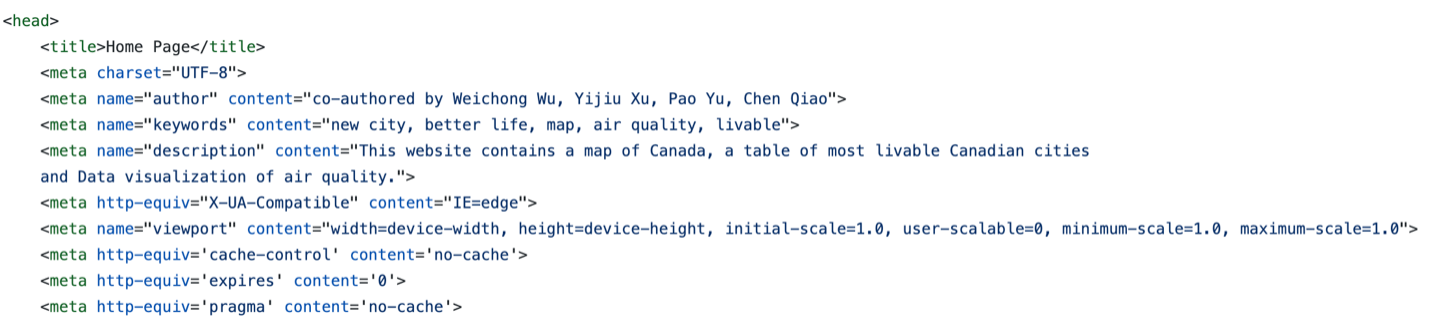
\includegraphics[width=6in]{images/q11.png}
	\caption{Meta tags of home page}
 \end{figure}

 \newpage

% =====================================================================
%   12. RESPONSIVENESS ON MOVILE AND OTHER PLATFORMS
% =====================================================================
\section{Responsiveness On Mobile and Other Platforms}

We used Bootstrap template \\(included here:https://qiao6.myweb.cs.uwindsor.ca/project/styles/bootstrap.css) 
\\For index page, aside from bootstrap, we also used CSS grids and CSS Media Queries. 
We tested on different platforms (macOS, windows, Linux Ubuntu, iPhone, Android):

\begin{figure}[htbp]
	\centering
	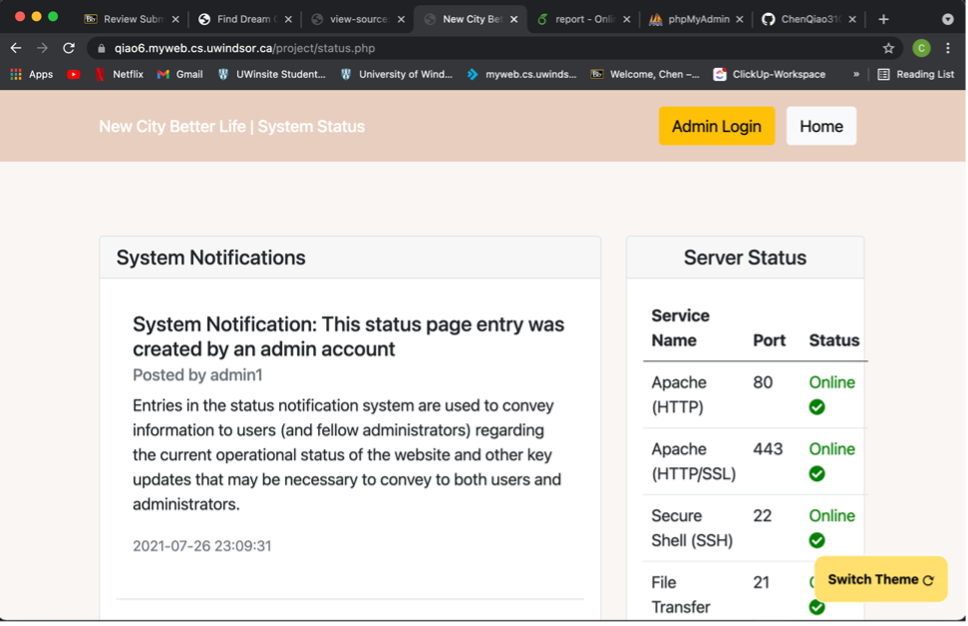
\includegraphics[width=4in]{images/q12-macOS.png}
	\caption{macOS}
 \end{figure}
 
 \begin{figure}[htbp]
	\centering
	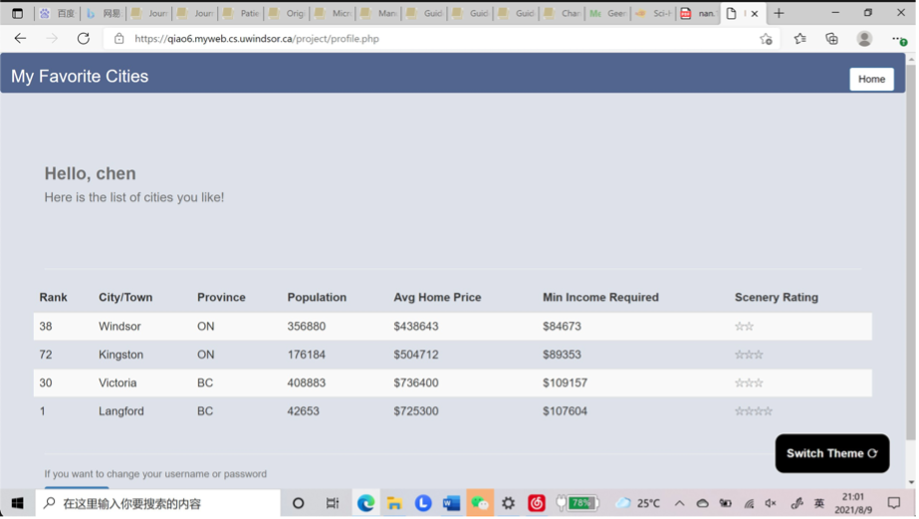
\includegraphics[width=4in]{images/q12-windows.png}
	\caption{windows}
 \end{figure}

 \newpage
 
 \begin{figure}[htbp]
	\centering
	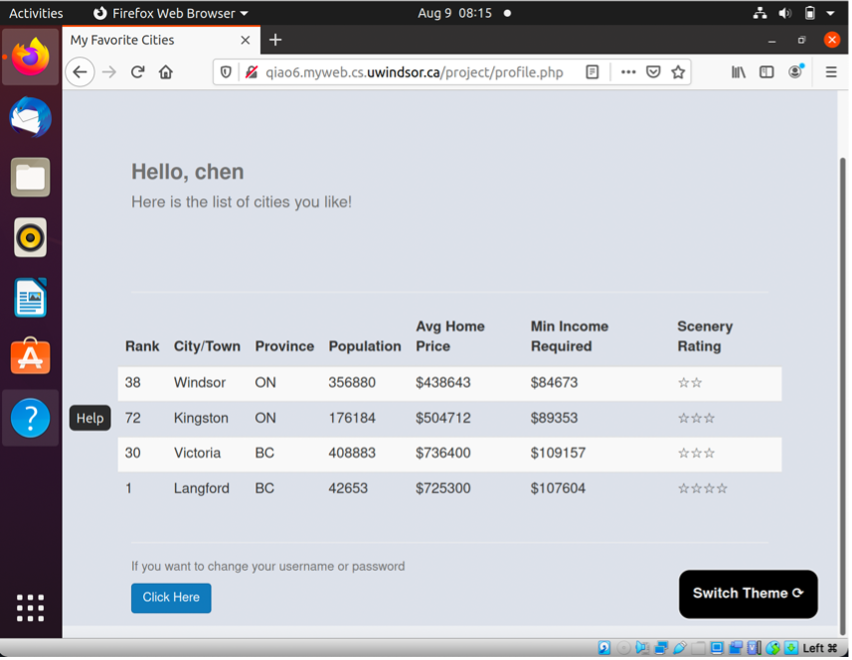
\includegraphics[width=4in]{images/q12linuxUbuntu.png}
	\caption{Linux Ubuntu}
 \end{figure}
 
 \newpage
 
 \begin{figure}[htbp]
	\centering
	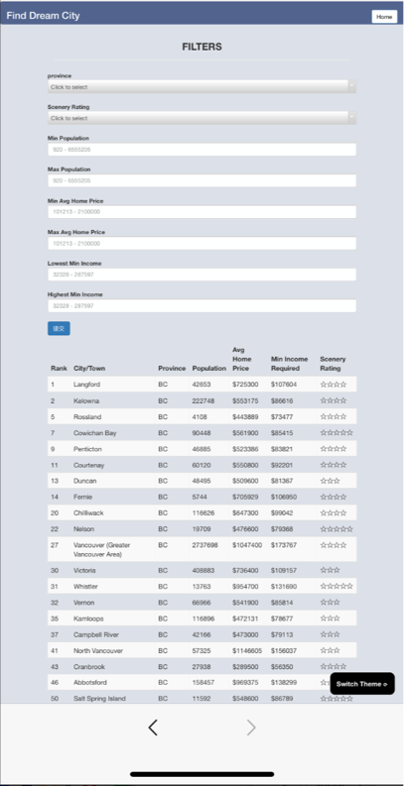
\includegraphics[width=1.4in]{images/q12-iphone.png}
	\caption{iPhone}
 \end{figure}
 
 \begin{figure}[htbp]
	\centering
	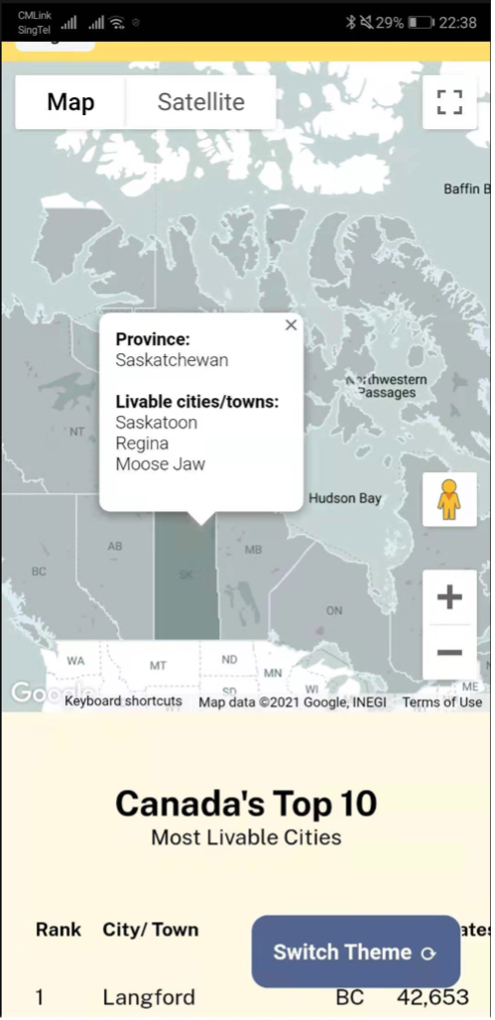
\includegraphics[width=1.4in]{images/q12-android.png}
	\caption{Android}
 \end{figure}
 
 \newpage


% =====================================================================
%  13. END-USER TRAINING
% =====================================================================
\section{End-User Training}
In addition to the general documentation, we made a 5 minute video:
\\https://www.youtube.com/watch?v=0FBFpGkqyig
\\We also created training step by step document to educate users on how the site works: 
\\https://pyxn.gitbook.io/newcitybetterlife/end-user-documentation/end-user-access
\\https://pyxn.gitbook.io/newcitybetterlife/end-user-documentation/end-user-city-information
\\https://pyxn.gitbook.io/newcitybetterlife/end-user-documentation/end-user-city-favourites
\\https://pyxn.gitbook.io/newcitybetterlife/end-user-documentation/end-user-update-account-info

 \begin{figure}[htbp]
	\centering
	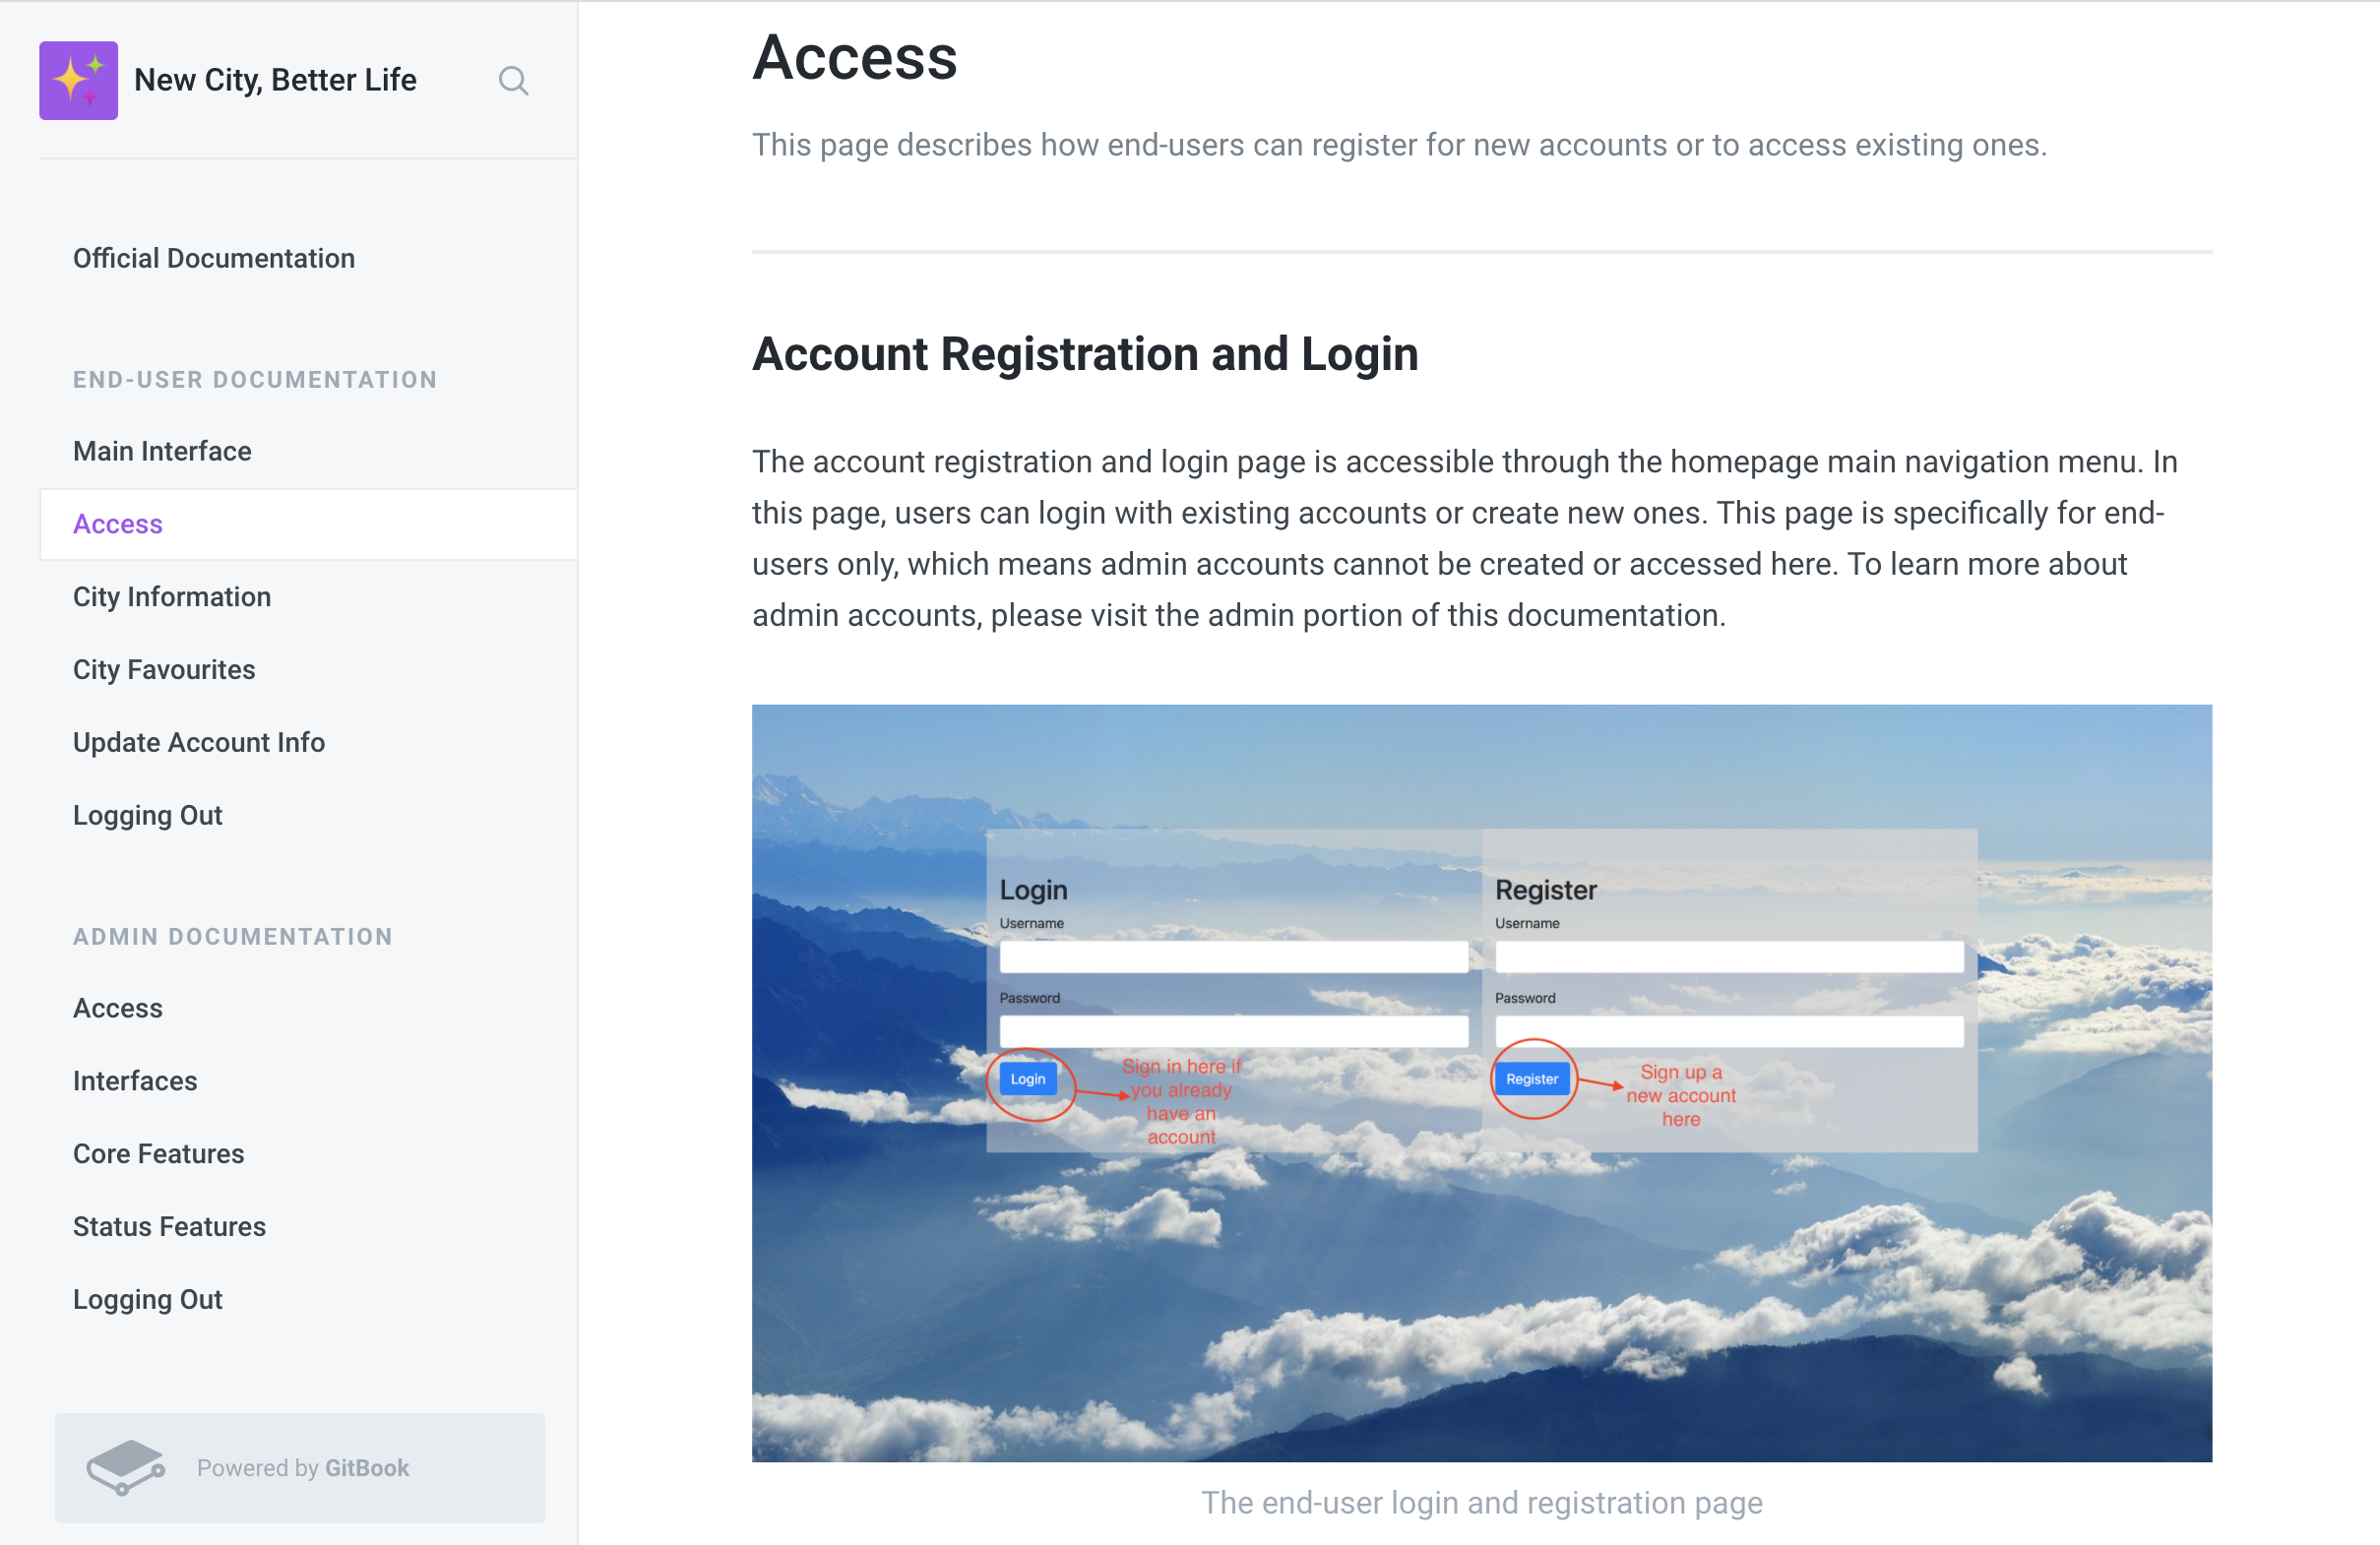
\includegraphics[width=4in]{images/q13.png}
	\caption{end-user training video}
 \end{figure}
 
 \begin{figure}[htbp]
	\centering
	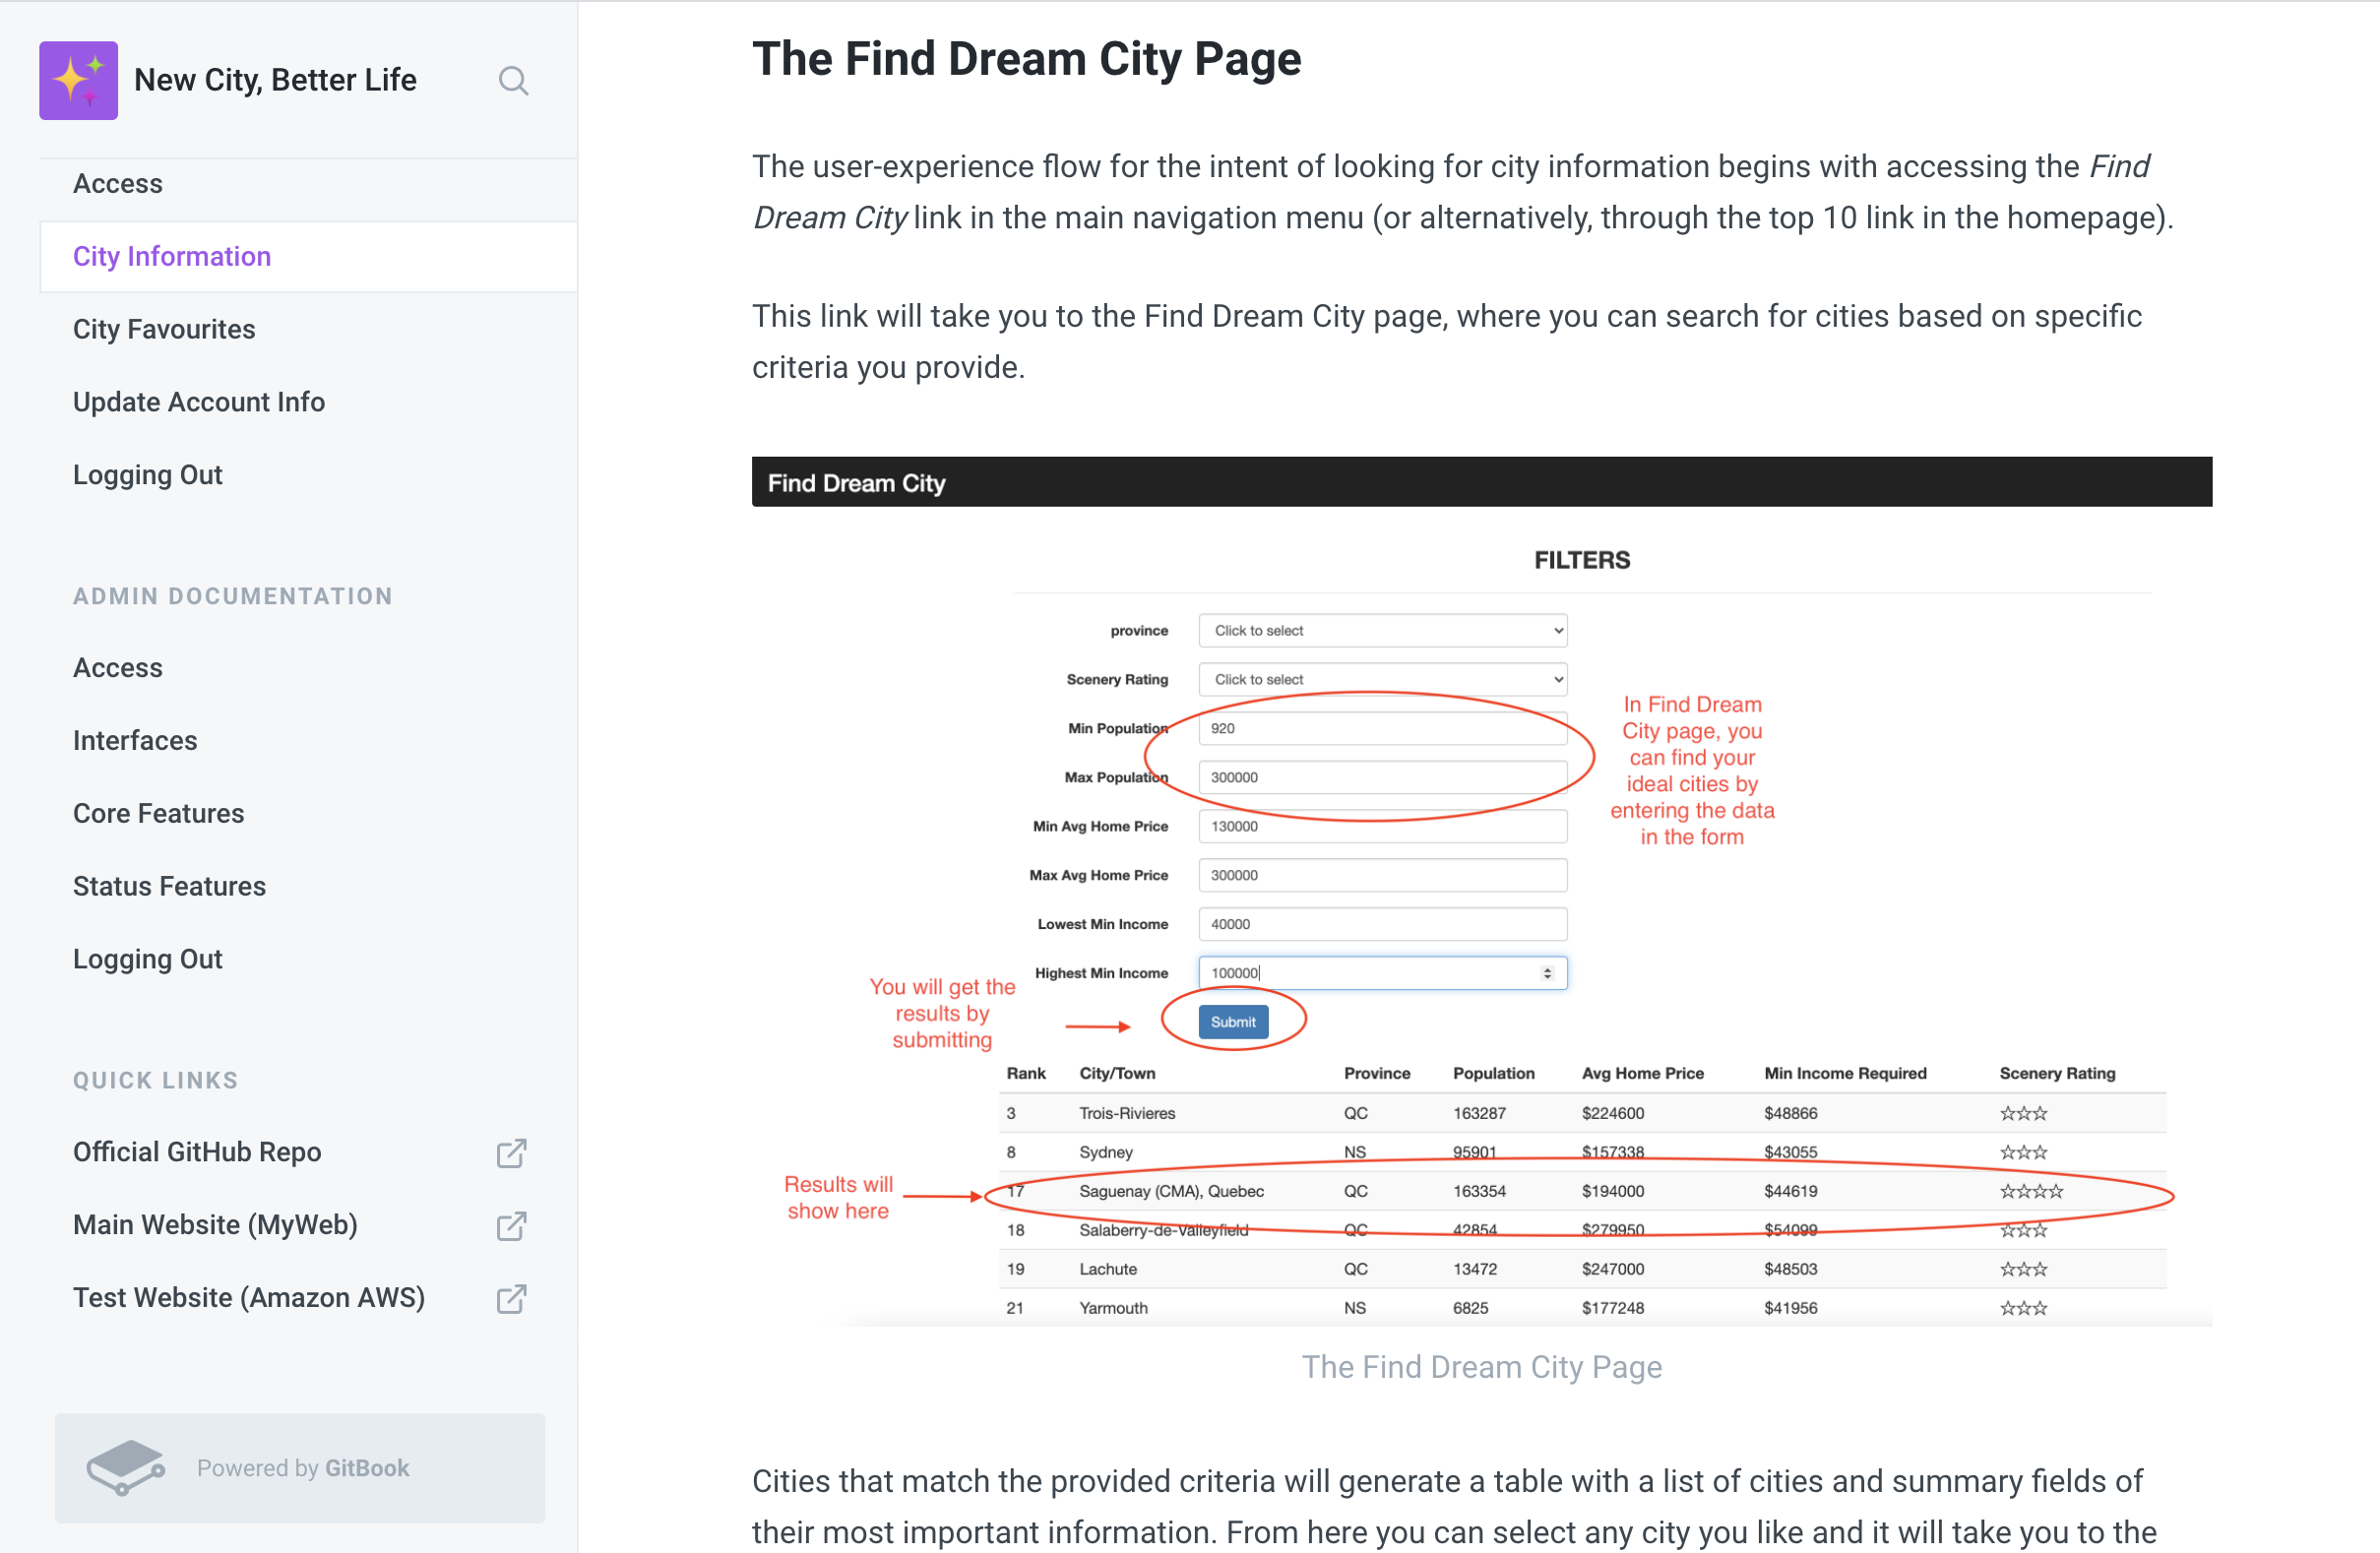
\includegraphics[width=4in]{images/q13-2.png}
	\caption{end-user training documentation}
 \end{figure}
 
 \newpage

% =====================================================================
%   14. ENABLE SWITCHING 3 SITE TEMPLATES
% =====================================================================
\section{Enable Switching 3 Site Templates}
After admin user logging in, he/she can select not only among 3 colour schemes that will impact the admin interface, but also 3 colour schemes that will impact the entire site. 

\begin{figure}[htbp]
	\centering
	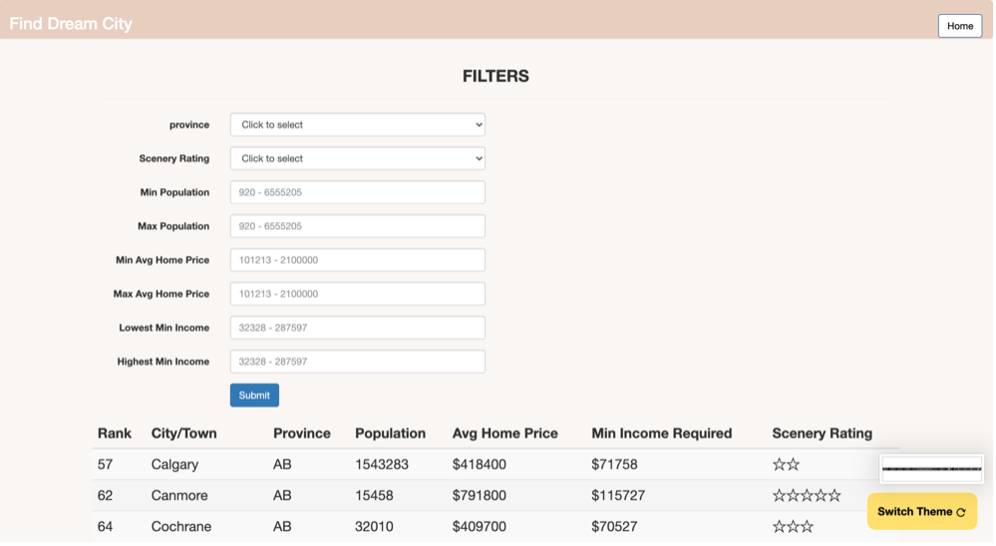
\includegraphics[width=3.1in]{images/q14-1.png}
	\caption{entire site scheme 1}
 \end{figure}
 
 \begin{figure}[htbp]
	\centering
	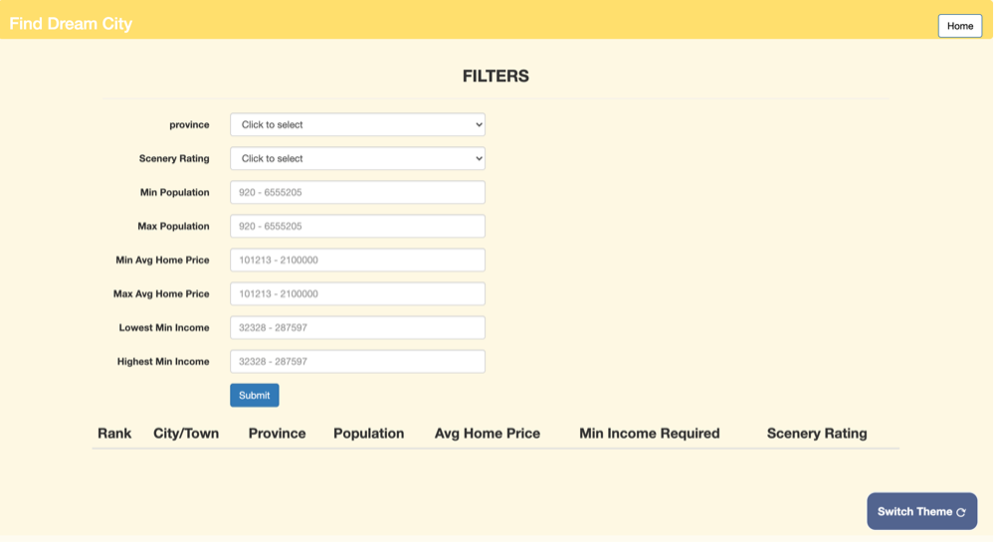
\includegraphics[width=3.1in]{images/q14-2png.png}
	\caption{entire site scheme 2}
 \end{figure}

\begin{figure}[htbp]
	\centering
	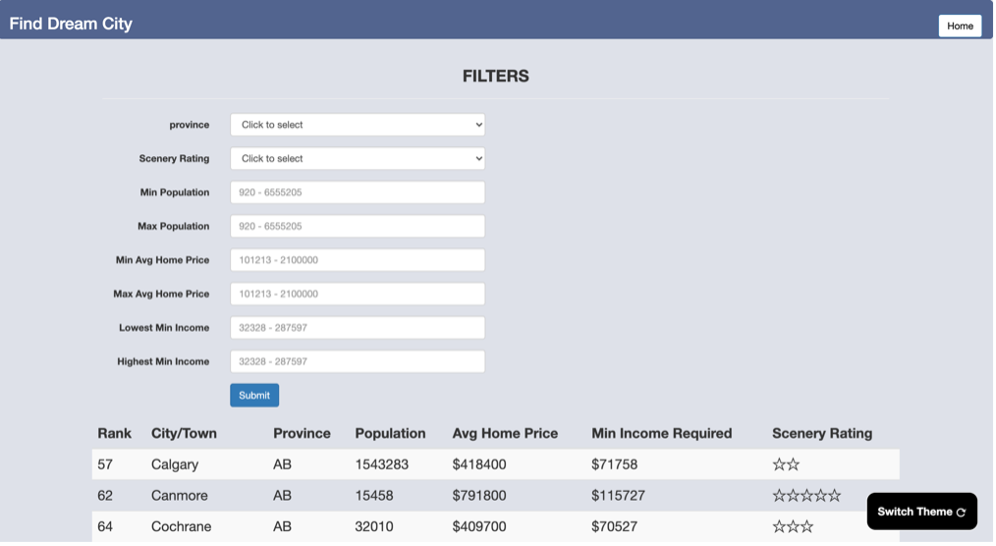
\includegraphics[width=3.1in]{images/q14-3.png}
	\caption{entire site scheme 3}
 \end{figure}
 \newpage
 
 \begin{figure}[htbp]
	\centering
	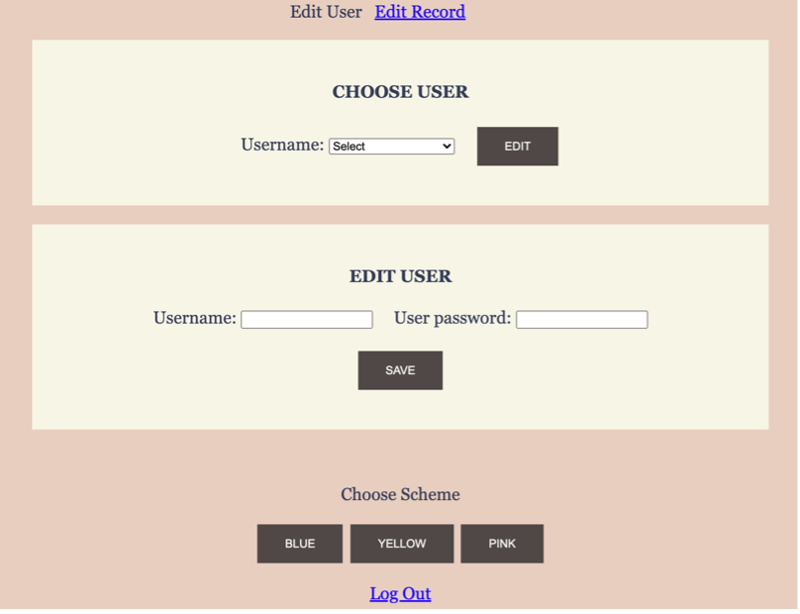
\includegraphics[width=3.7in]{images/q14-4.png}
	\caption{admin interface scheme 1}
 \end{figure}
 
 \begin{figure}[htbp]
	\centering
	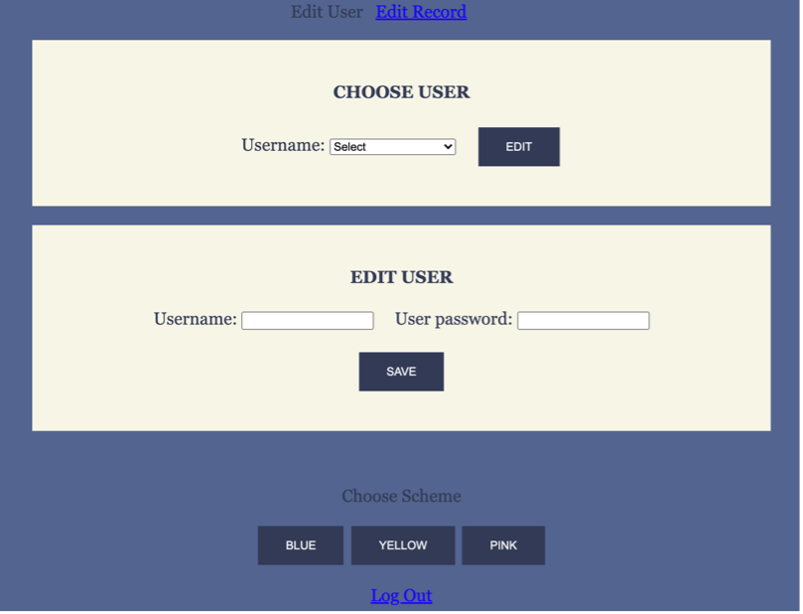
\includegraphics[width=3.7in]{images/q14-5.png}
	\caption{admin interface scheme 2}
 \end{figure}
 
 \newpage

\begin{figure}[htbp]
	\centering
	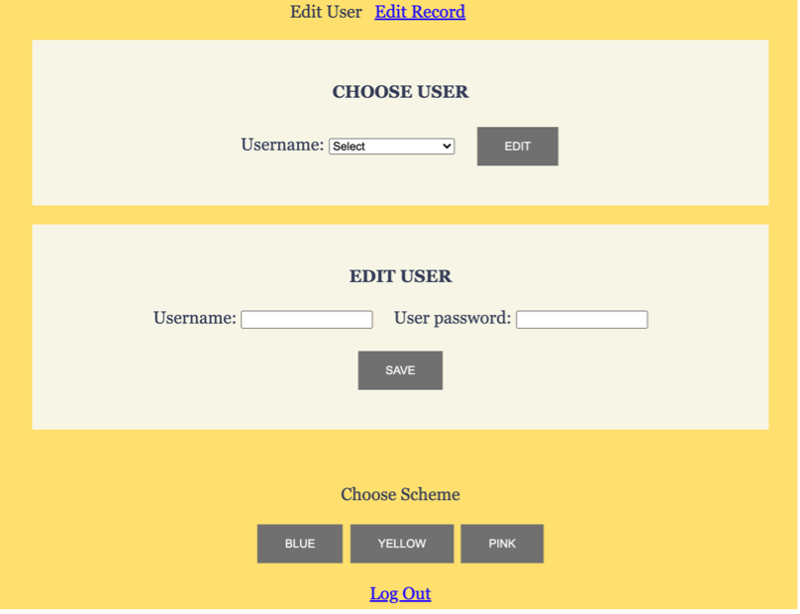
\includegraphics[width=3.7in]{images/q14-6.png}
	\caption{admin interface scheme 3}
 \end{figure}
 \newpage

% =====================================================================
%   15. DATABASE USED
% =====================================================================
\section{Database Used}
MySQL database used with 6 tables created:

\begin{figure}[htbp]
	\centering
	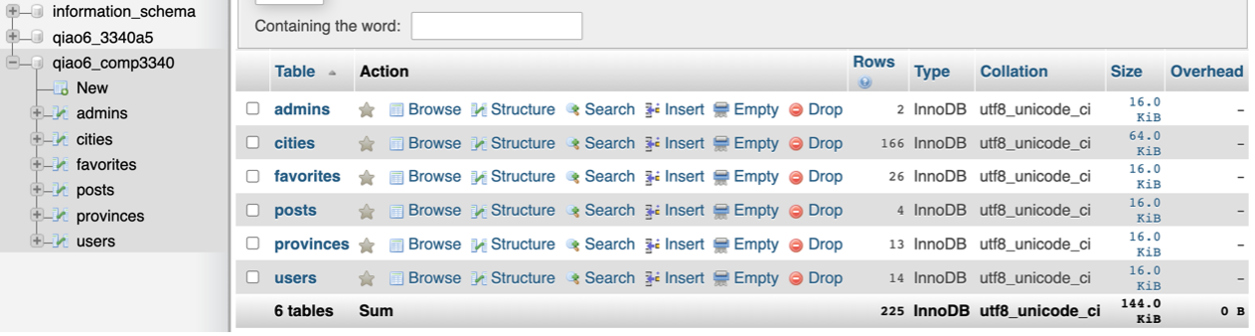
\includegraphics[width=6in]{images/q15.png}
	\caption{Database Tables}
 \end{figure}

 \newpage

% =====================================================================
%   16. DATA RECORD MANIPULATIONS
% =====================================================================
\section{Data Record Manipulations}
We used "insert", "select", "update" SQL queries. 
Here are some sample commands from the PHP code for each:

\begin{figure}[htbp]
	\centering
	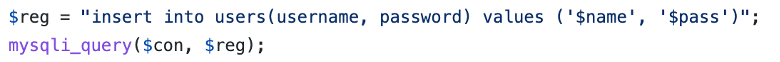
\includegraphics[width=6in]{images/q16-1.png}
	\caption{SQL inserts a new record into table called "users" }
 \end{figure}
 
 \begin{figure}[htbp]
	\centering
	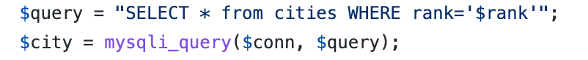
\includegraphics[width=6in]{images/q16-2.png}
	\caption{SQL selects a city record from our table “favorites” }
 \end{figure}
 
 \begin{figure}[htbp]
	\centering
	
\includegraphics[width=6in]{images/q16-3.png}
	
\includegraphics[width=6in]{images/q16-4.png}
	\caption{SQL updates a user record in table “cities” }
 \end{figure}

 \newpage

% =====================================================================
%   17. USER MANAGEMENT
% =====================================================================
\section{User Management}
Admin user can edit user records. After editing user record, the corresponding record in “favorite” table will be updated as well.  Admin user can also edit city records.

\begin{figure}[htbp]
	\centering
	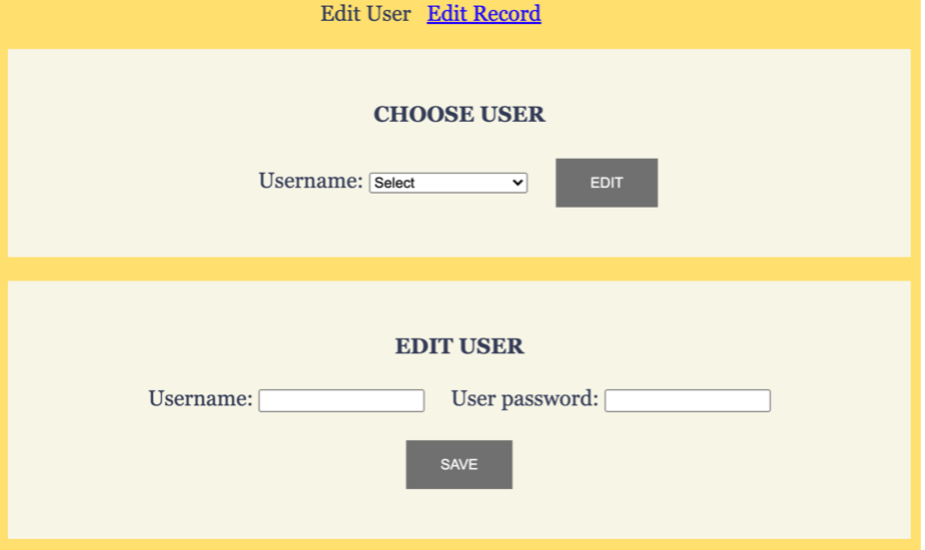
\includegraphics[width=3in]{images/q17-1.png}
	\caption{Admin user can edit user records}
 \end{figure}
 
 \begin{figure}[htbp]
	\centering
	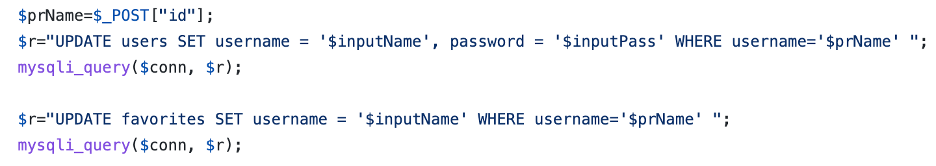
\includegraphics[width=4in]{images/q17-2.png}
	\caption{The corresponding record in “favorite” table will be updated}
 \end{figure}
 
 \begin{figure}[htbp]
	\centering
	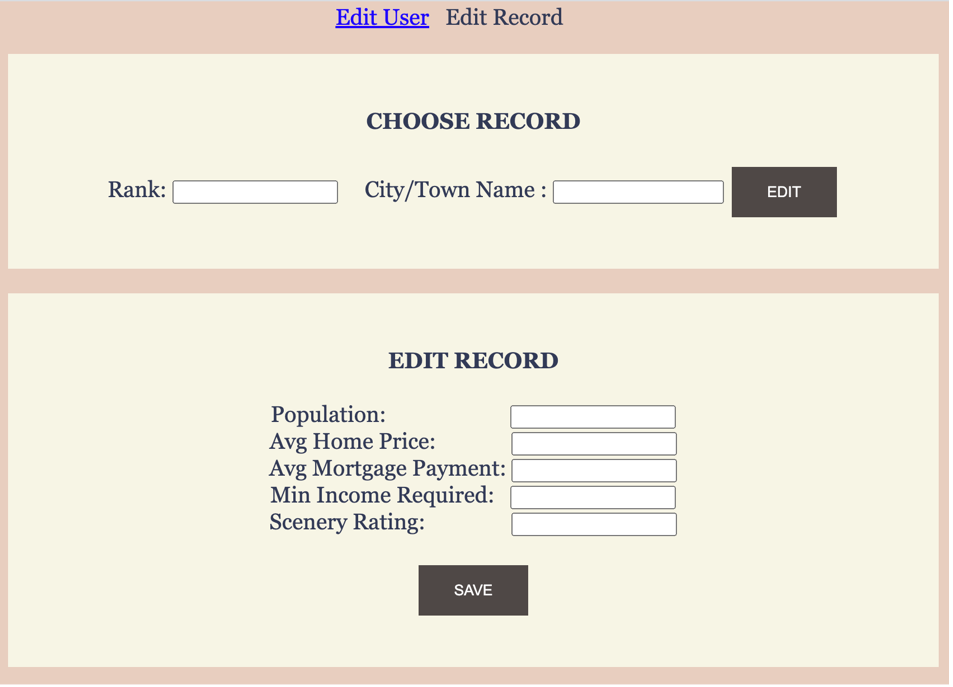
\includegraphics[width=3in]{images/q17-3.png}
	\caption{Admin user can also edit city records}
 \end{figure}

 \newpage

% =====================================================================
%   18. ADMIN DOCUMENTATION
% =====================================================================
\section{Admin Documentation}
https://pyxn.gitbook.io/newcitybetterlife/admin-documentation/access
\\https://pyxn.gitbook.io/newcitybetterlife/admin-documentation/admin-interface
\\https://pyxn.gitbook.io/newcitybetterlife/admin-documentation/core-features
\\used to provide the admin with the details and use of the admin features.

\begin{figure}[htbp]
	\centering
	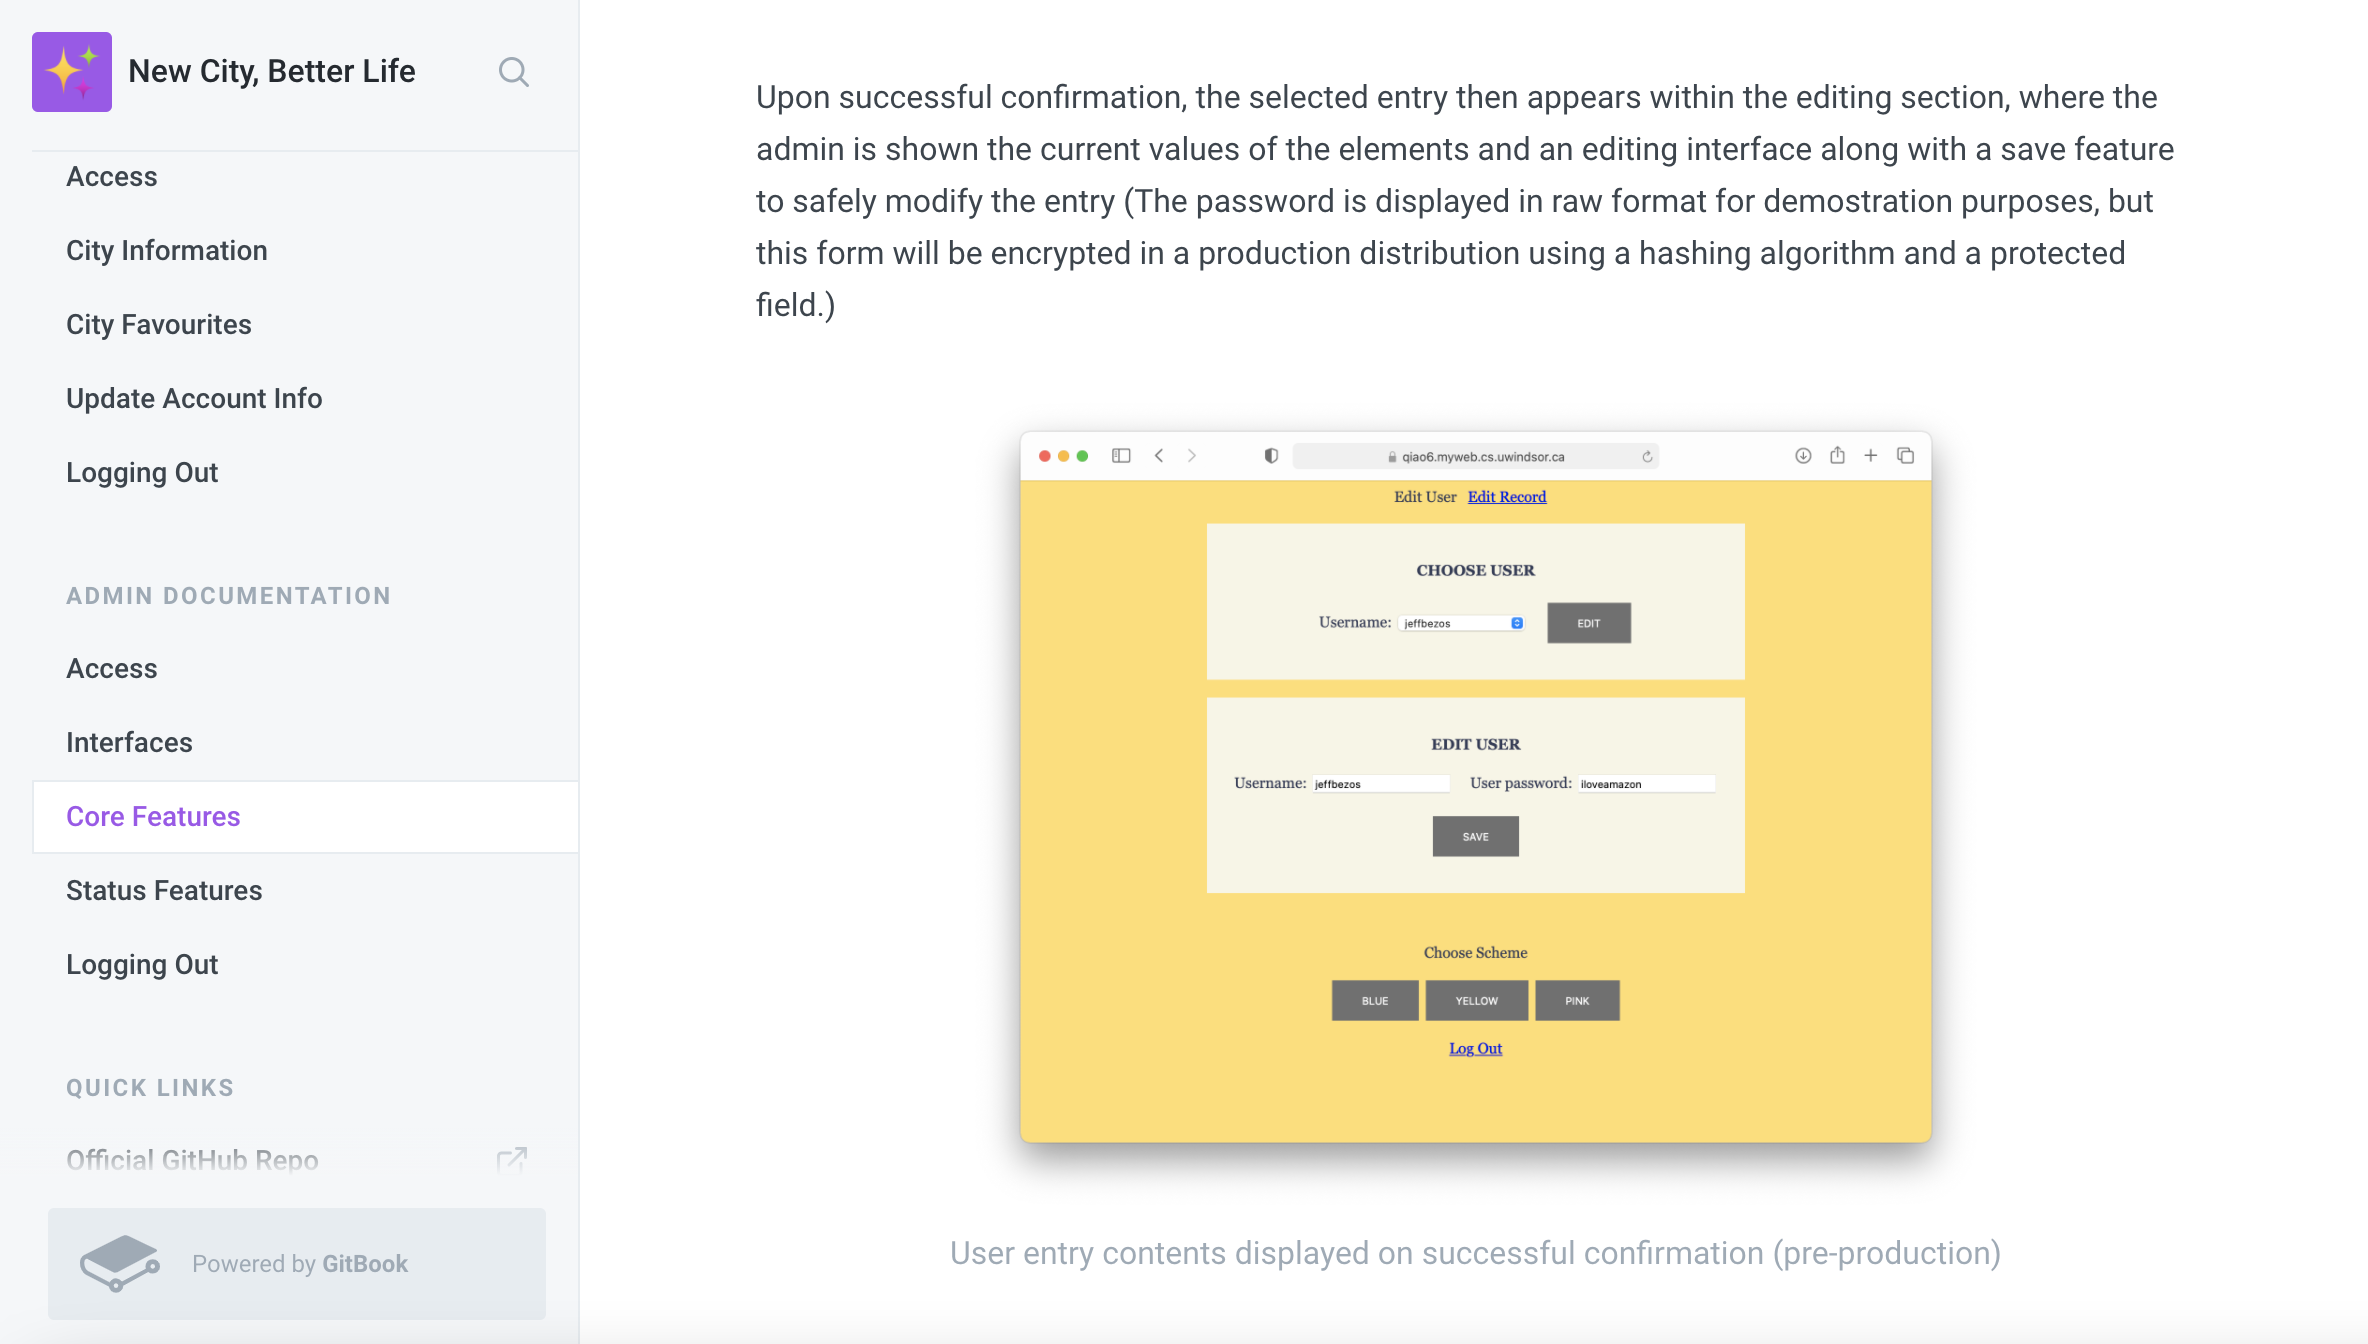
\includegraphics[width=5in]{images/q18-1.png}
	\caption{Edit user/city record}
 \end{figure}
 
 \begin{figure}[htbp]
	\centering
	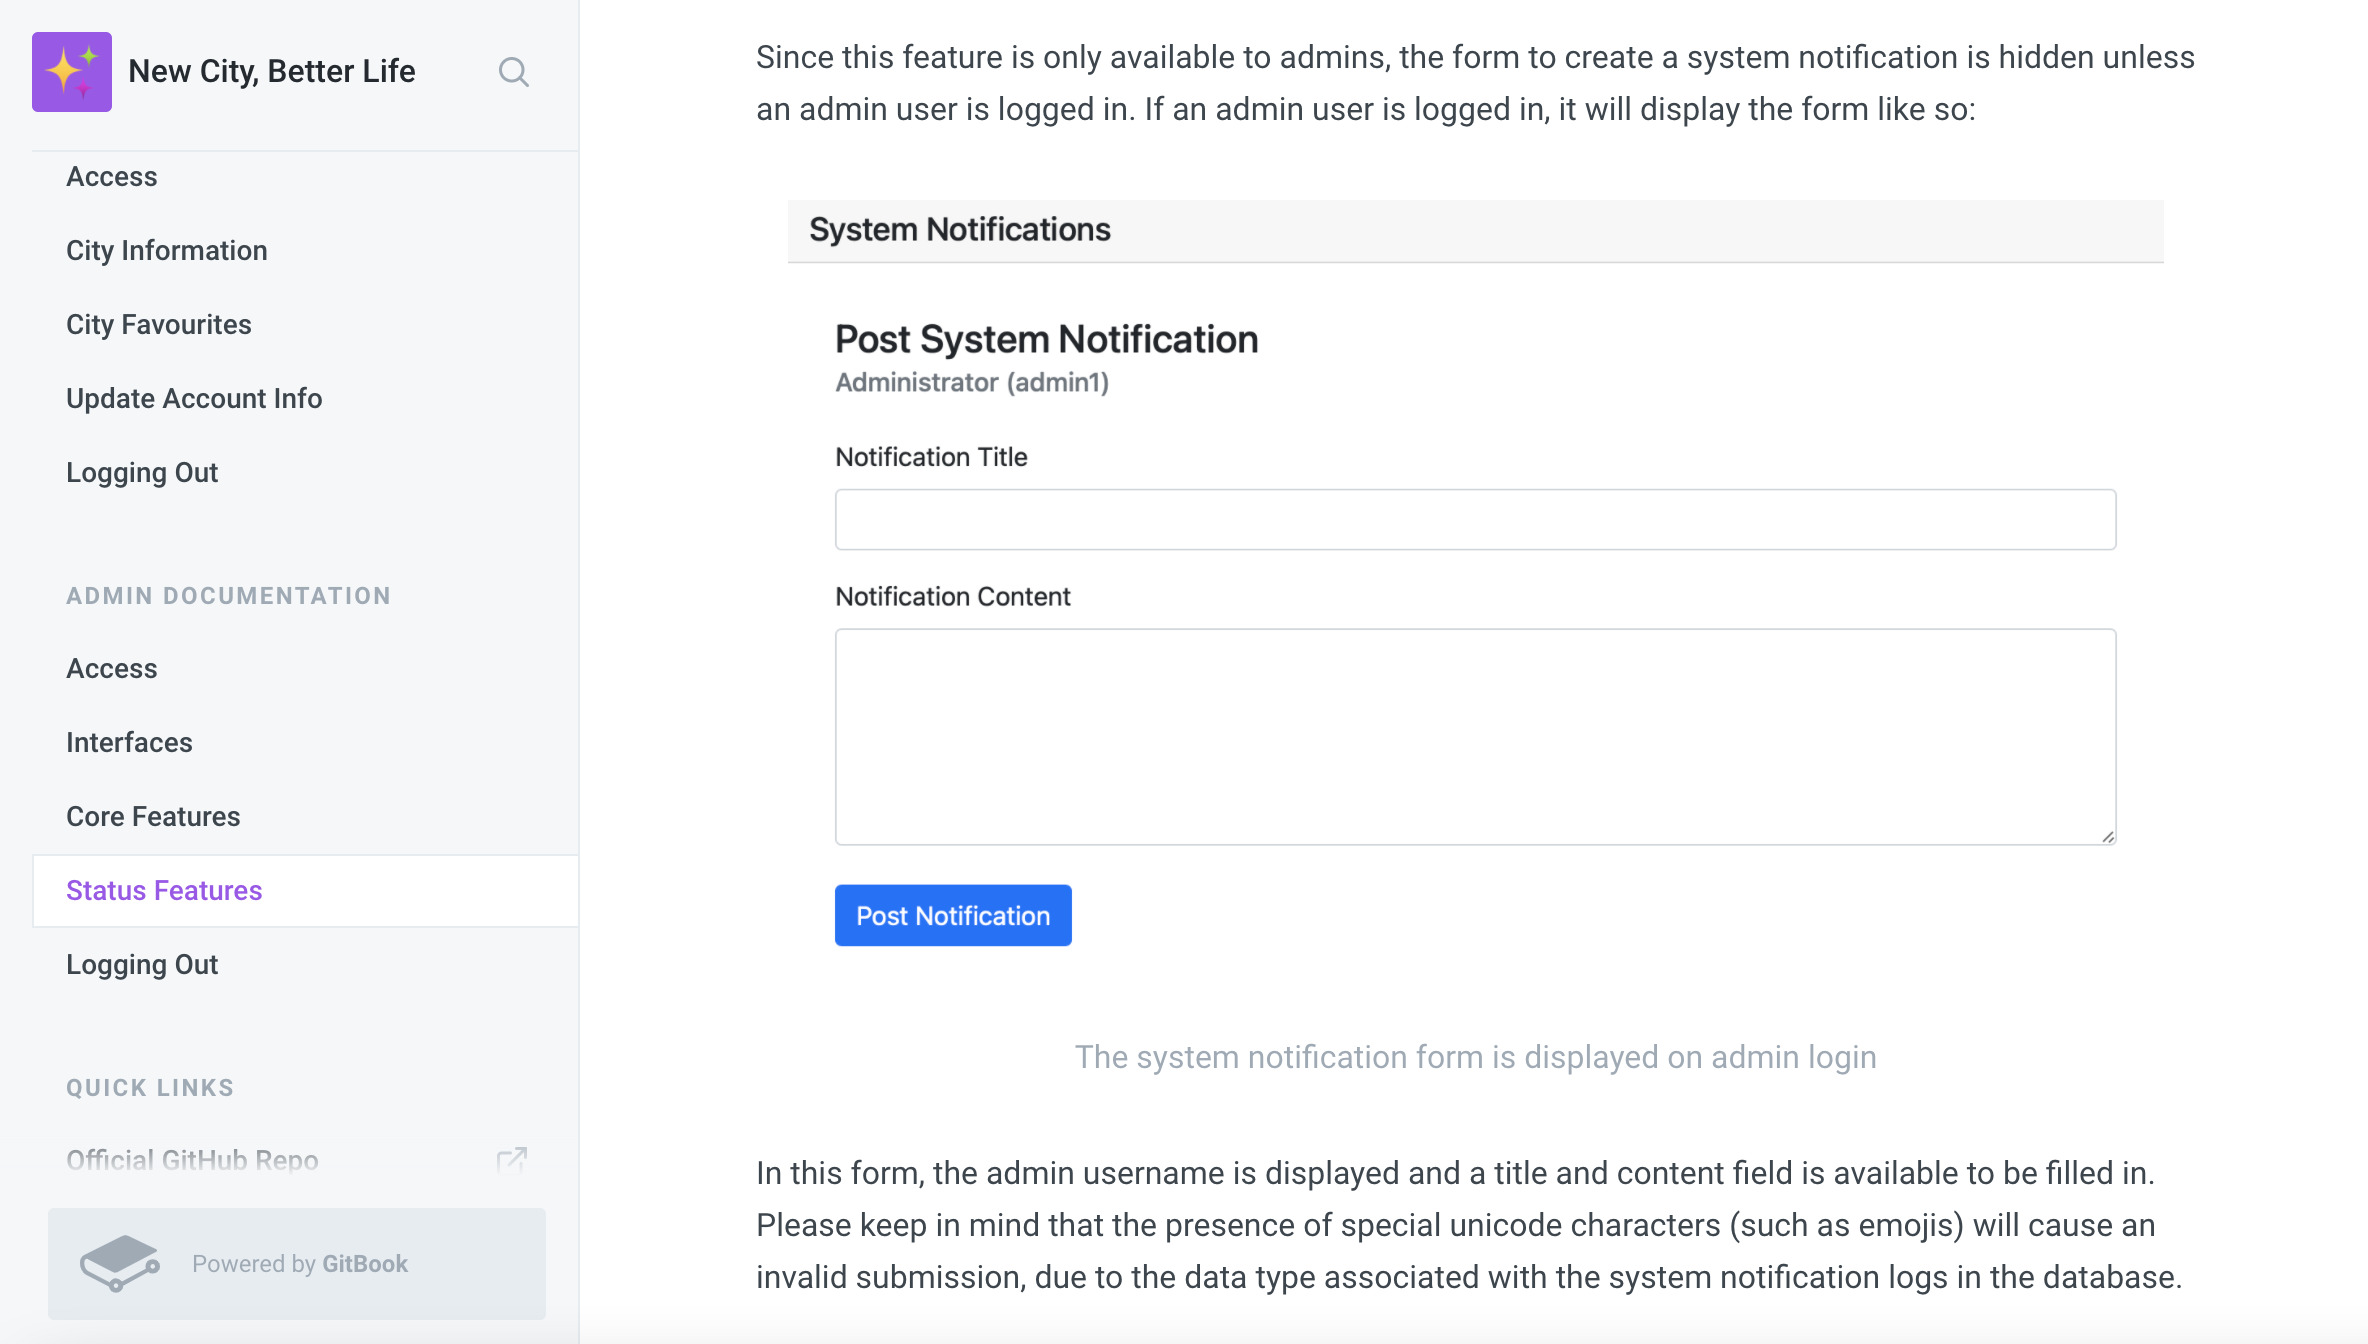
\includegraphics[width=5in]{images/q18-2.png}
	\caption{Post system notification}
 \end{figure}

 \newpage

% =====================================================================
%   19. STATUS AND MONITORING PAGE
% =====================================================================
\section{Status \& Monitoring Page}
https://qiao6.myweb.cs.uwindsor.ca/project/status.php
\\This page tests to see if the Database, File Transfer, Secure Shell, Apache and Internet Connection are working (green), it shows red otherwise. This page also provide a notification posting function for admin users.

\begin{figure}[htbp]
	\centering
	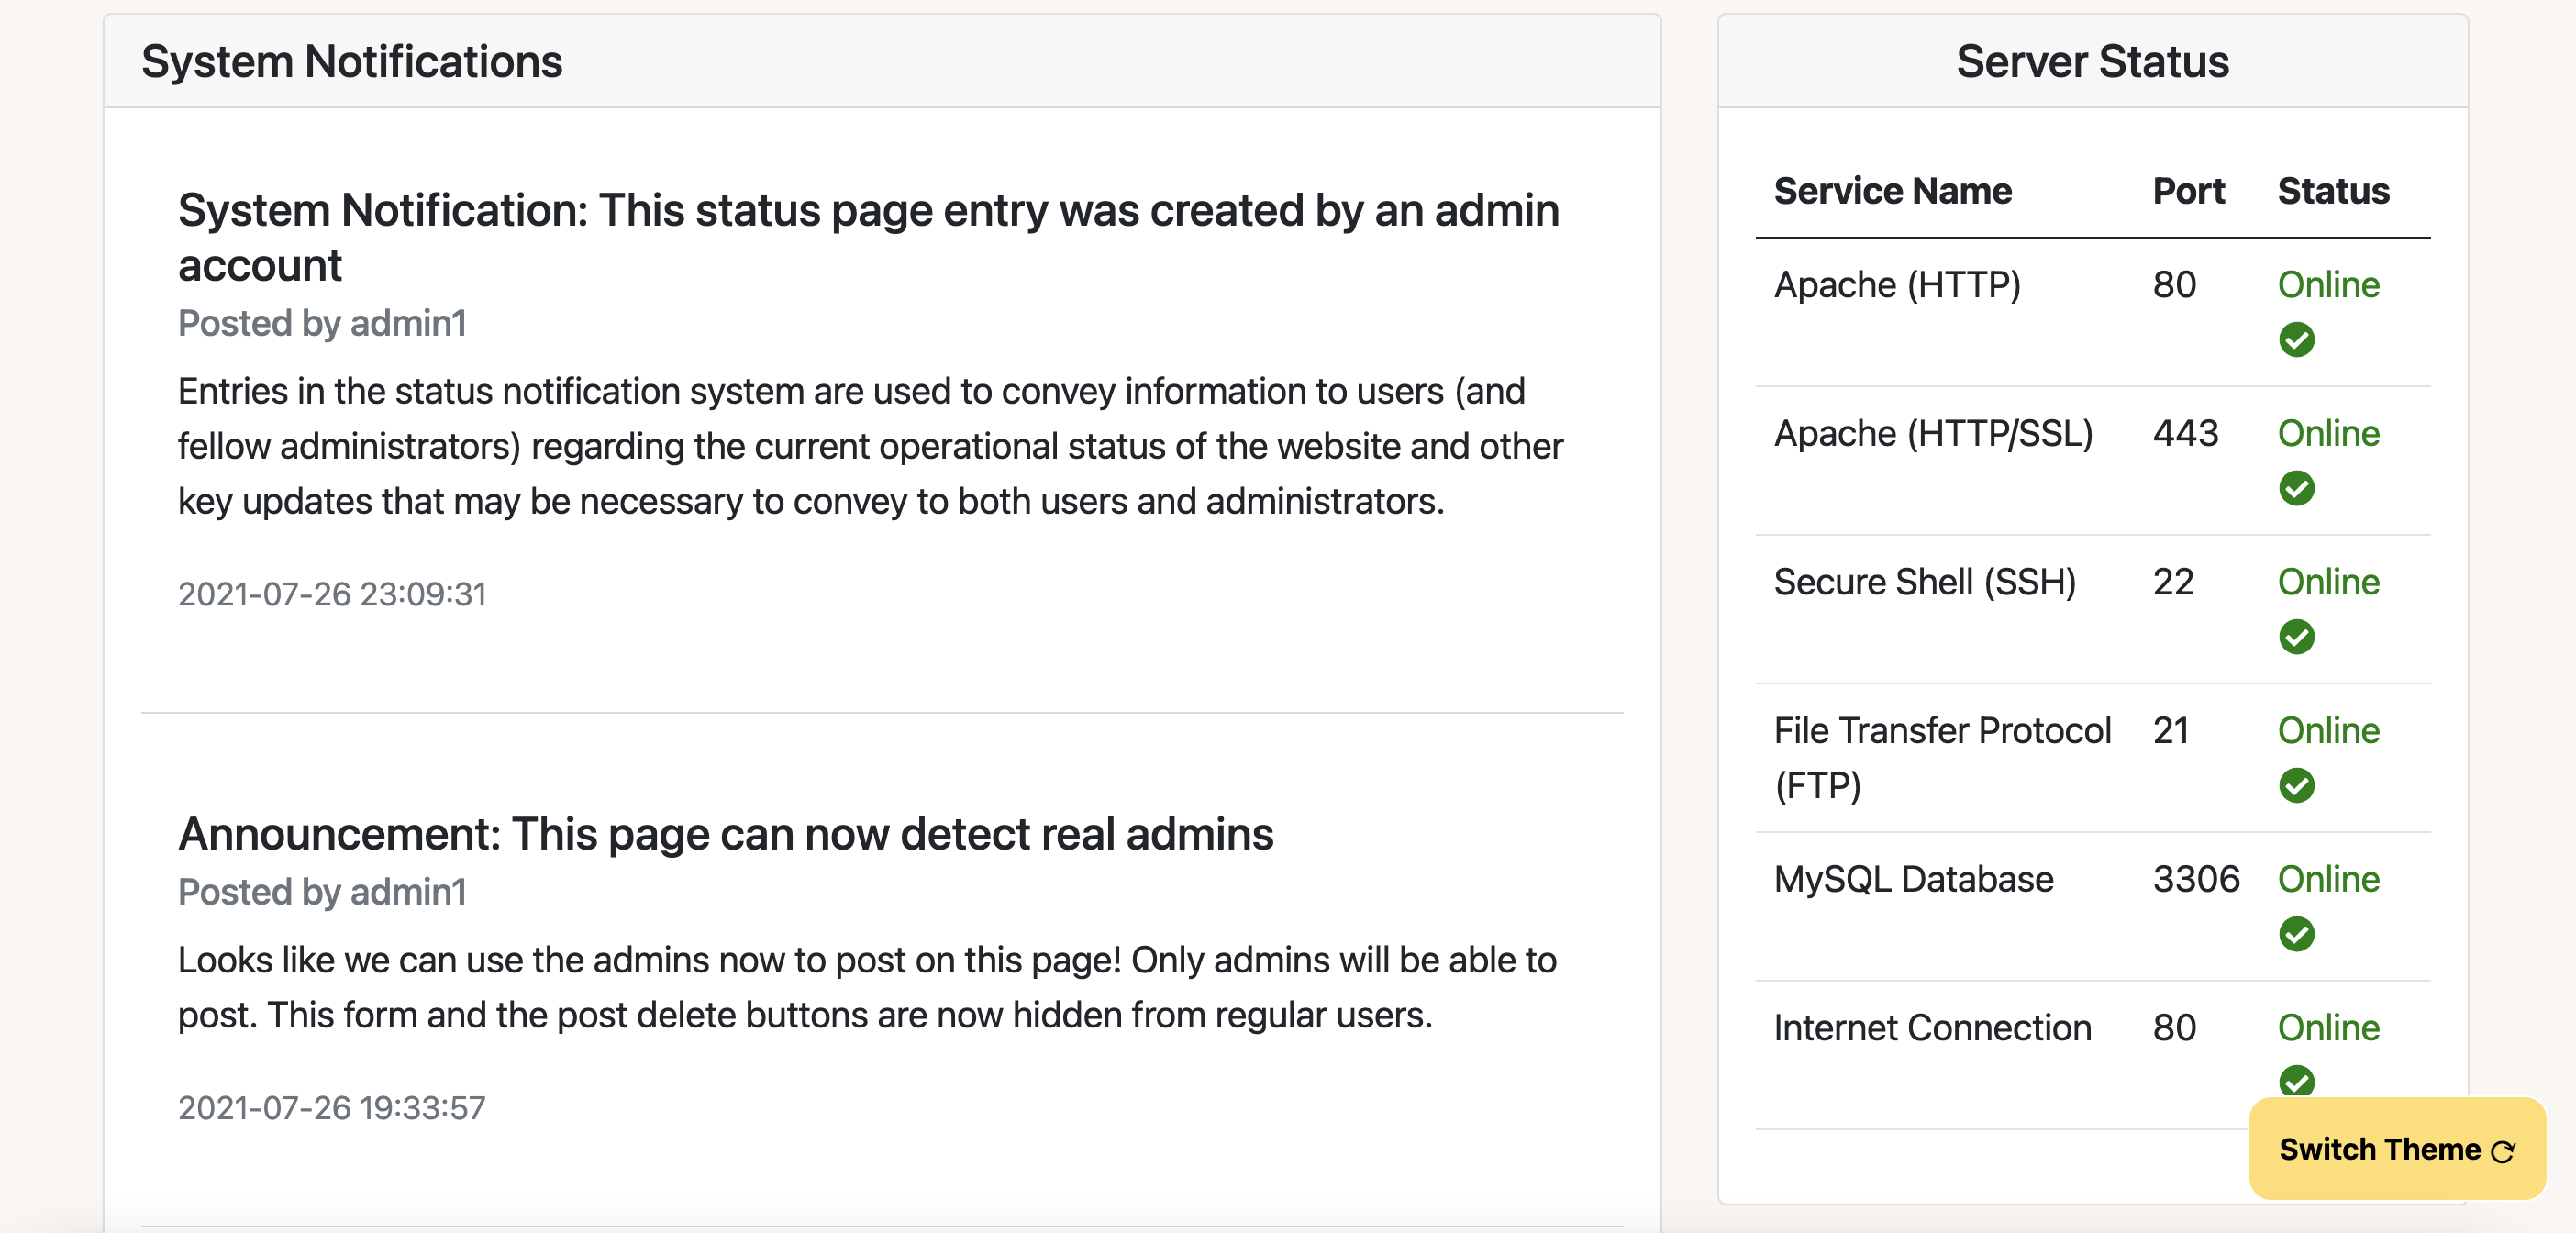
\includegraphics[width=5in]{images/q19.png}
	\caption{Status \& monitoring page}
 \end{figure}

 \newpage

% =====================================================================
%   20. DATABASE RECORDS
% =====================================================================
\section{Database Records}
The table "cities" has 166 records, the table "provinces" has 13 records. 
The number of records is shown in the cardinality colum:

\begin{figure}[htbp]
	\centering
	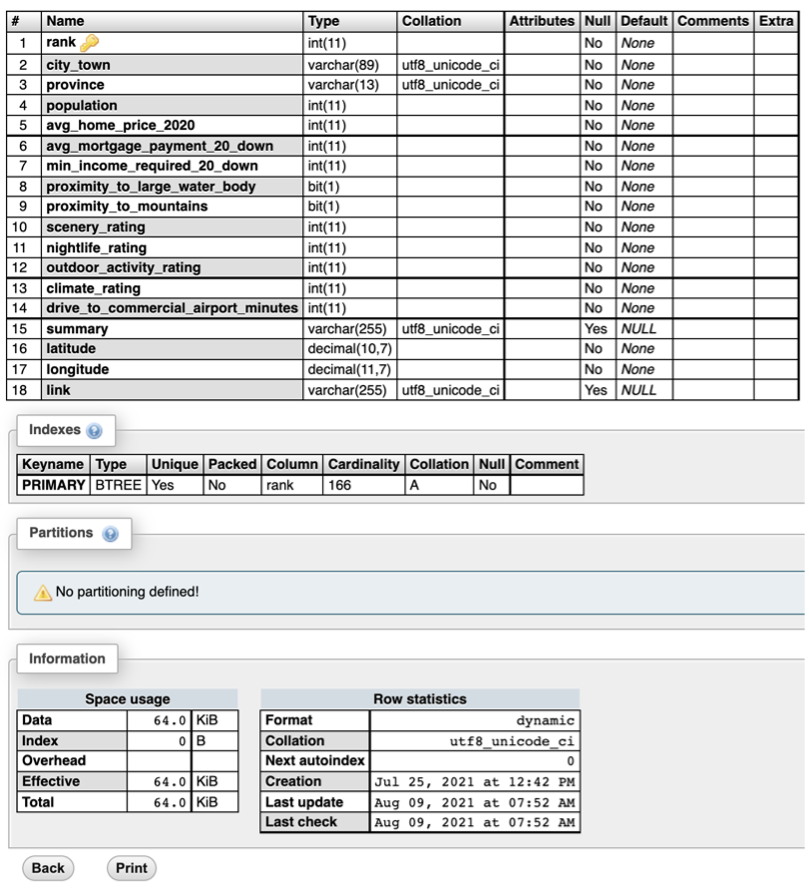
\includegraphics[width=2.5in]{images/q20-1.png}
	\caption{table "cities" has 166 records}
 \end{figure}


\begin{figure}[htbp]
	\centering
	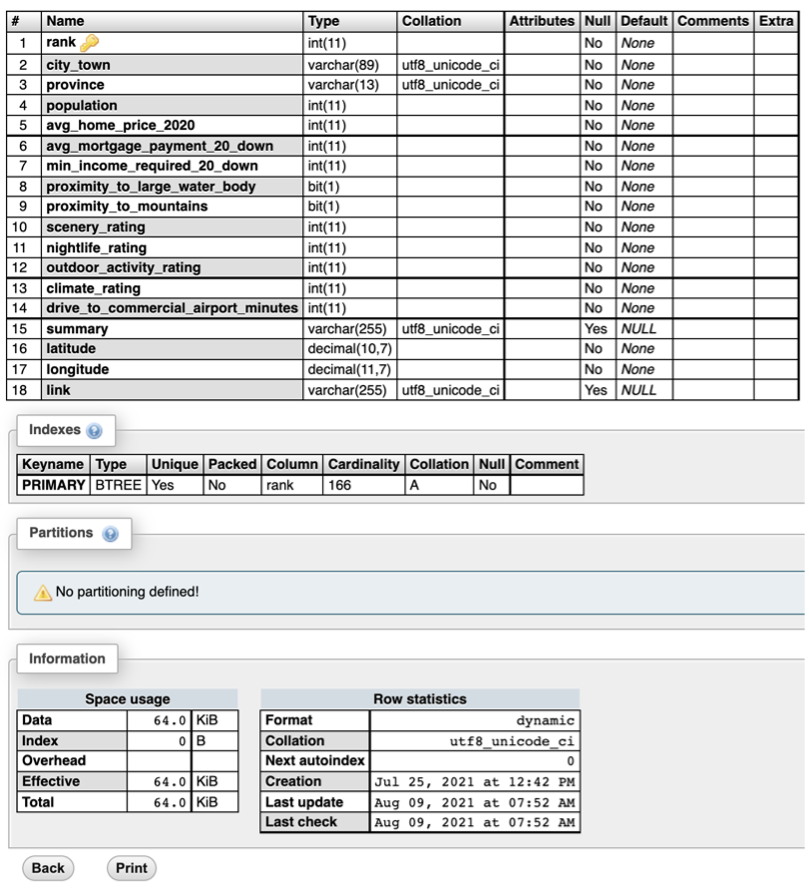
\includegraphics[width=2.5in]{images/q20-2.png}
	\caption{table "provinces" has 13 records}
 \end{figure}
 \newpage

% =====================================================================
%   21. OPEN DATA SET
% =====================================================================
\section{Open Data Set}

\subsection*{Air Quality Data by Canadian Province}
For our open dataset, we used one of the Government of Canada's official datasets. The data set is from \textit{Environment and Climate Change Canada} deparment, and describes air quality monitoring data gathered by the \textit{National Air Pollution Surveillance Program} (NAPS) from the years 1974 to 2020. To make this dataset more relevant to our audience, we opted to only include data from the most recent year available, 2020.

\subsection*{Dataset URL}
The URL for the complete dataset can be found here \url{https://data-donnees.ec.gc.ca/data/air/monitor/national-air-pollution-surveillance-naps-program/Data-Donnees/?lang=en}.

\begin{figure}[htbp]
	\centering
	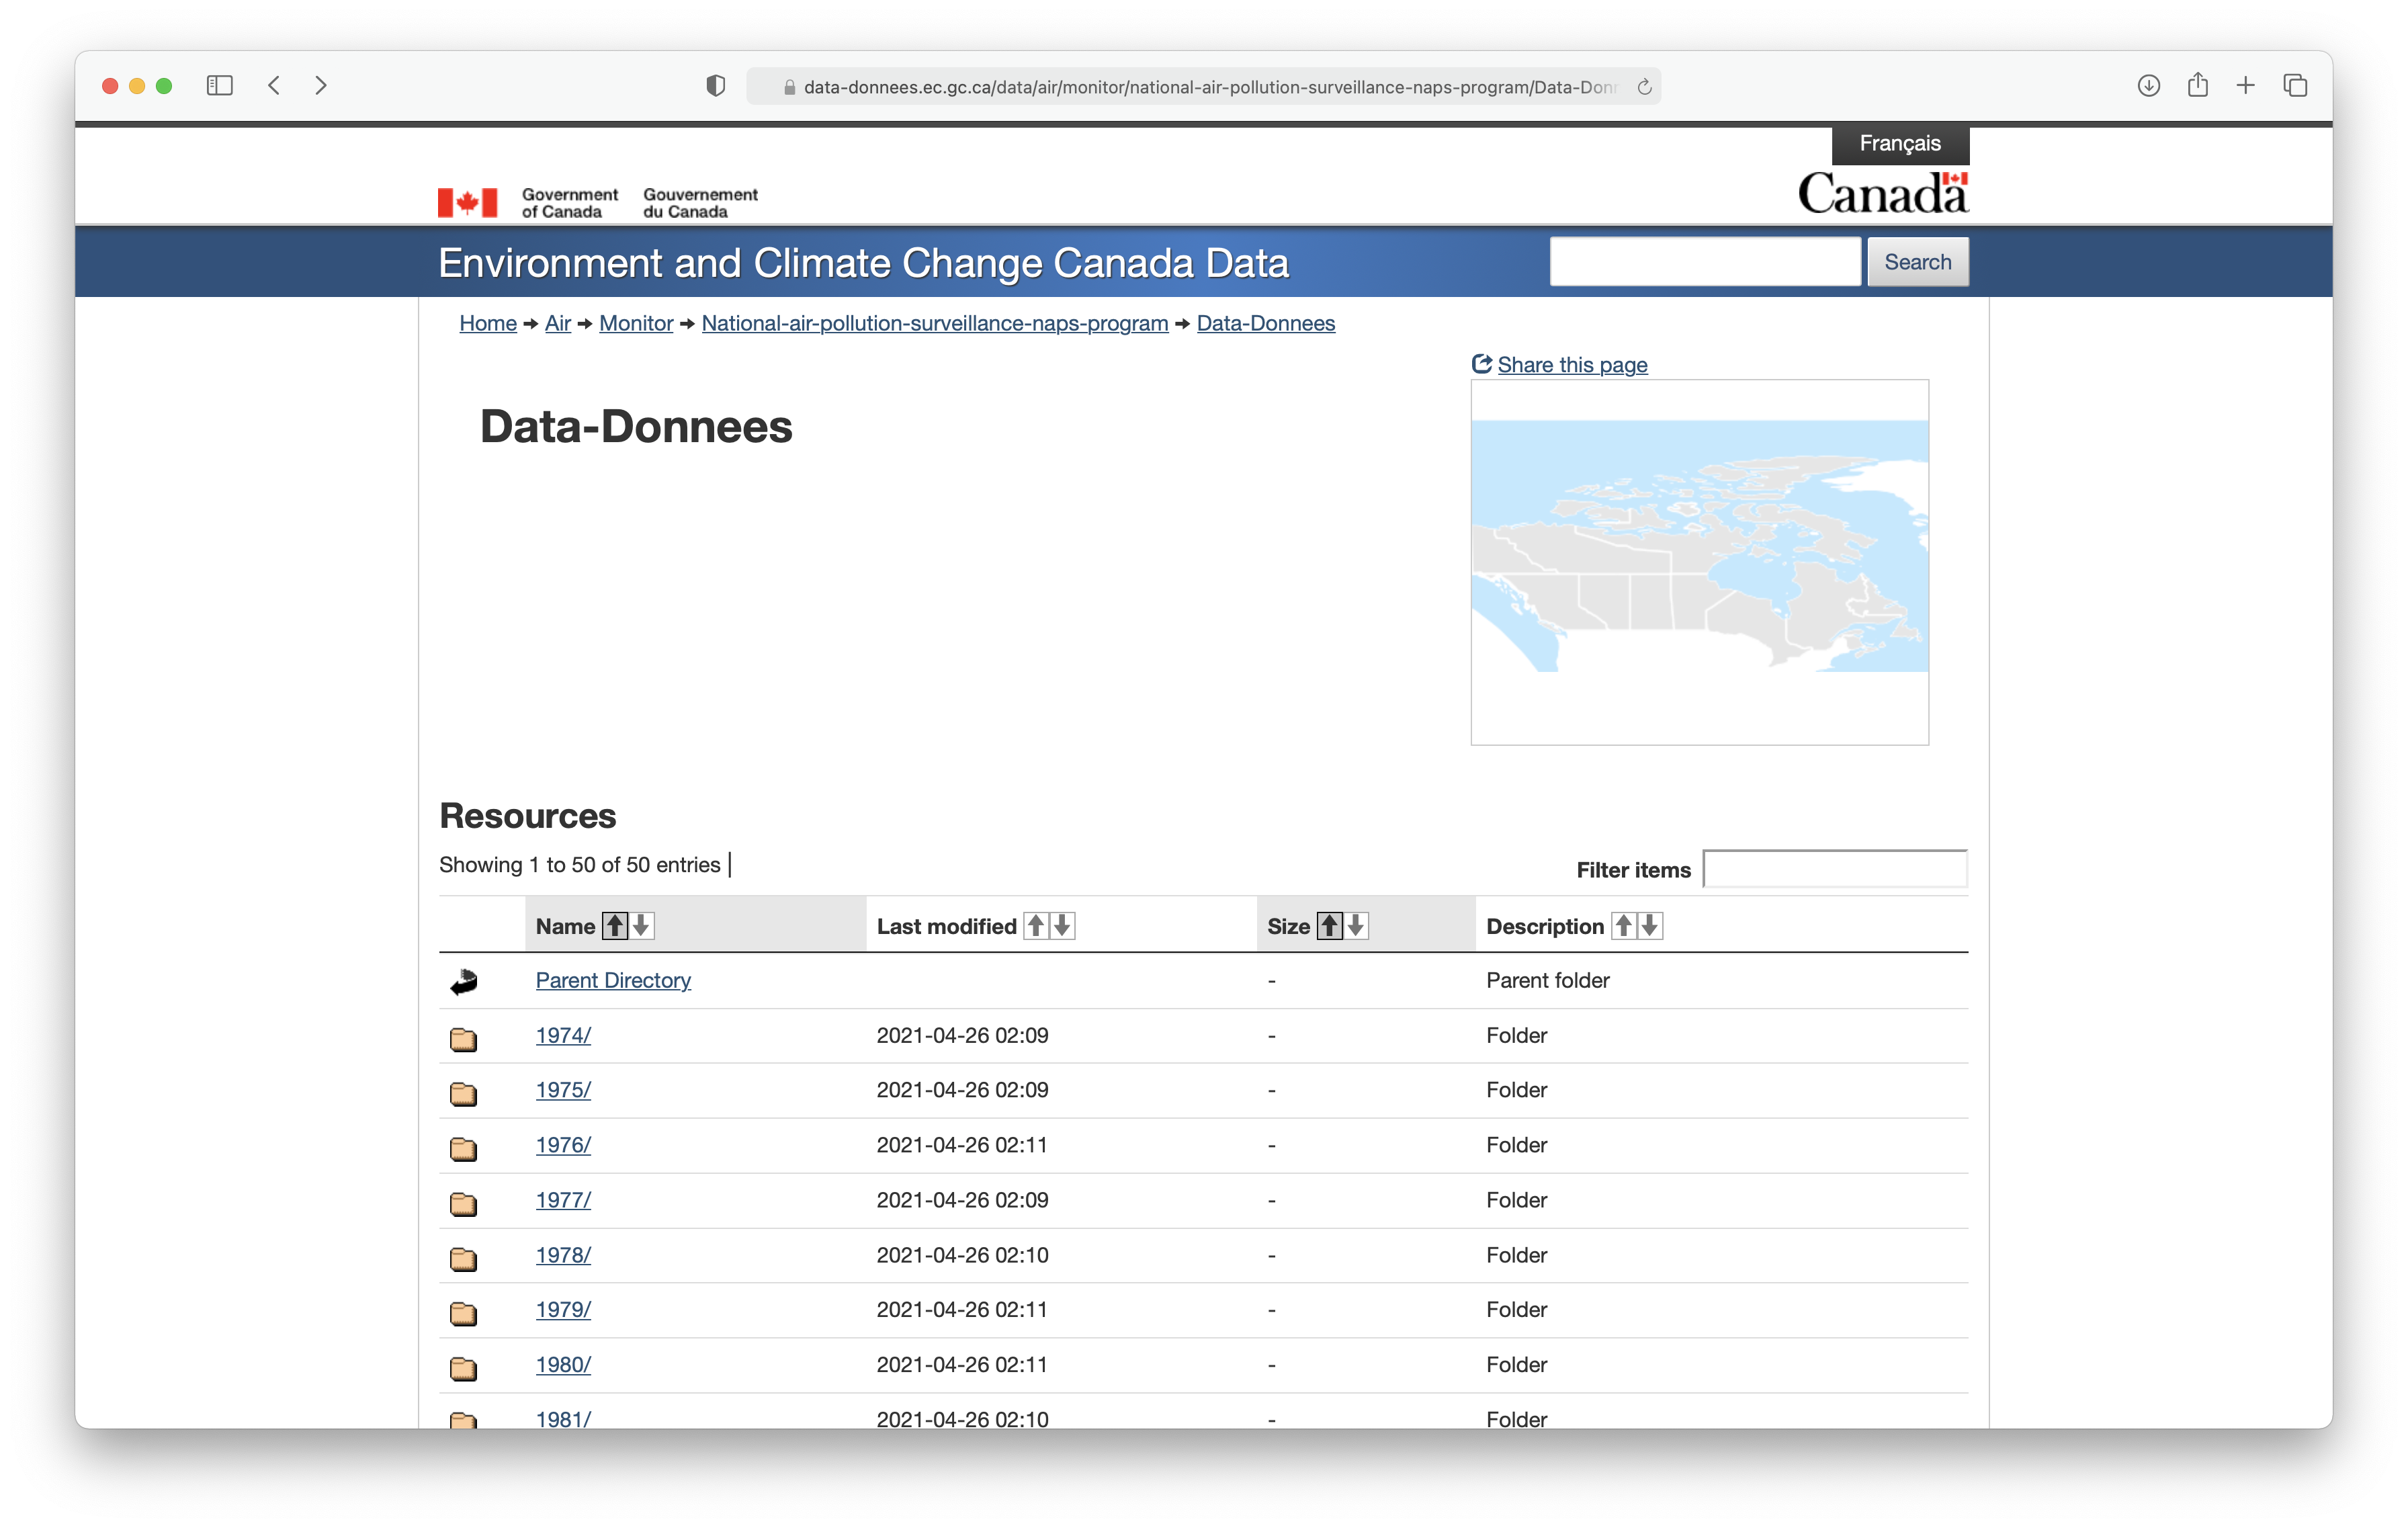
\includegraphics[width=\textwidth]{images/21-1-opendataset.png}
	\caption{NAPS Program: Live Open Dataset}
 \end{figure}

\newpage

\subsection*{Code Implementation}
The open dataset was provided in separate CSV files (by city) and was manually reorganized, cleansed and formatted into a single CSV table. The table was then summarized using an Excel pivot table and the data directly applied to a JavaScript data visualization framework (Plotly.js) displayed below to maximize data visualization speed and performance:

\begin{lstlisting}[language=java]
var trace1 = {
	x: ['AB', 'BC', 'MB', 'NB', 'NL', 'NS', 'ON', 'PE', 'QC', 'SK', 'YU'],
	y: [5.764, 4.922, 3.614, 5.668, 3.657, 3.674, 6.182, 3.321, 6.545, 4.722, 2.588],
	type: 'bar',
	text: ['5.764(micro)g/m3', '4.922(micro)g/m3', '3.614(micro)g/m3', '5.668(micro)g/m3', '3.657(micro)g/m3', '3.674(micro)g/m3', '6.182(micro)g/m3', '3.321(micro)g/m3', '6.545(micro)g/m3', '4.722(micro)g/m3', '2.588(micro)g/m3'],
	marker: { color: '#ffcc99' }
};

var data = [trace1];

var titleCode = `
	<span id="airQualityTitle" style="font-family: 'Public Sans', sans-serif; font-size: 1.618rem; font-weight: bold;">
		Statistic data of PM2.5 
	</span>
	<br>
	<span id="airQualitySubtitle" style="font-family: 'Public Sans', sans-serif; font-size: 1rem;">
		Based on National Air Pollution <br> Surveillance (NAPS) Program
	</span>
`;

var layout = {
	title: titleCode,
	font: { family: 'Raleway, sans-serif' },
	showlegend: false,
	xaxis: { tickangle: -45 },
	yaxis: {
		zeroline: false,
		gridwidth: 2
	},
	bargap: 0.5
};

Plotly.newPlot('airQuality', data, layout);
\end{lstlisting}

 \newpage

% =====================================================================
%   22. PHP
% =====================================================================
\section{PHP}

A minimum of 5 scripts with documentation and 26 total PHP scripts were created at the time of this writing to make the website fully-operational with its current features.
\begin{enumerate}
	\item \lstinline{DatabaseHelper.php}
	\item \lstinline{ThemeHelper.php}
	\item \lstinline{adminlogin_editrecord.php}
	\item \lstinline{adminlogin_edituser.php}
	\item \lstinline{adminlogin_status.php}
	\item \lstinline{adminlogout.php}
	\item \lstinline{city.php}
	\item \lstinline{dreamcity.php}
	\item \lstinline{editrecord.php}
	\item \lstinline{edituser.php}
	\item \lstinline{favorite.php}
	\item \lstinline{index.php}
	\item \lstinline{login.php}
	\item \lstinline{logout.php}
	\item \lstinline{navigation.php}
	\item \lstinline{post.php}
	\item \lstinline{profile.php}
	\item \lstinline{registration.php}
	\item \lstinline{status.php}
	\item \lstinline{switchtheme.php}
	\item \lstinline{userchange.php}
	\item \lstinline{validation_editrecord.php}
	\item \lstinline{validation_edituser.php}
	\item \lstinline{validation_status.php}
	\item \lstinline{validation.php}
\end{enumerate}

\newpage
\subsection*{5 PHP Script Samples with Documentation}

%   Script 1
% ------------------------------------------------------------------------

\begin{figure}[htbp]
	\centering
	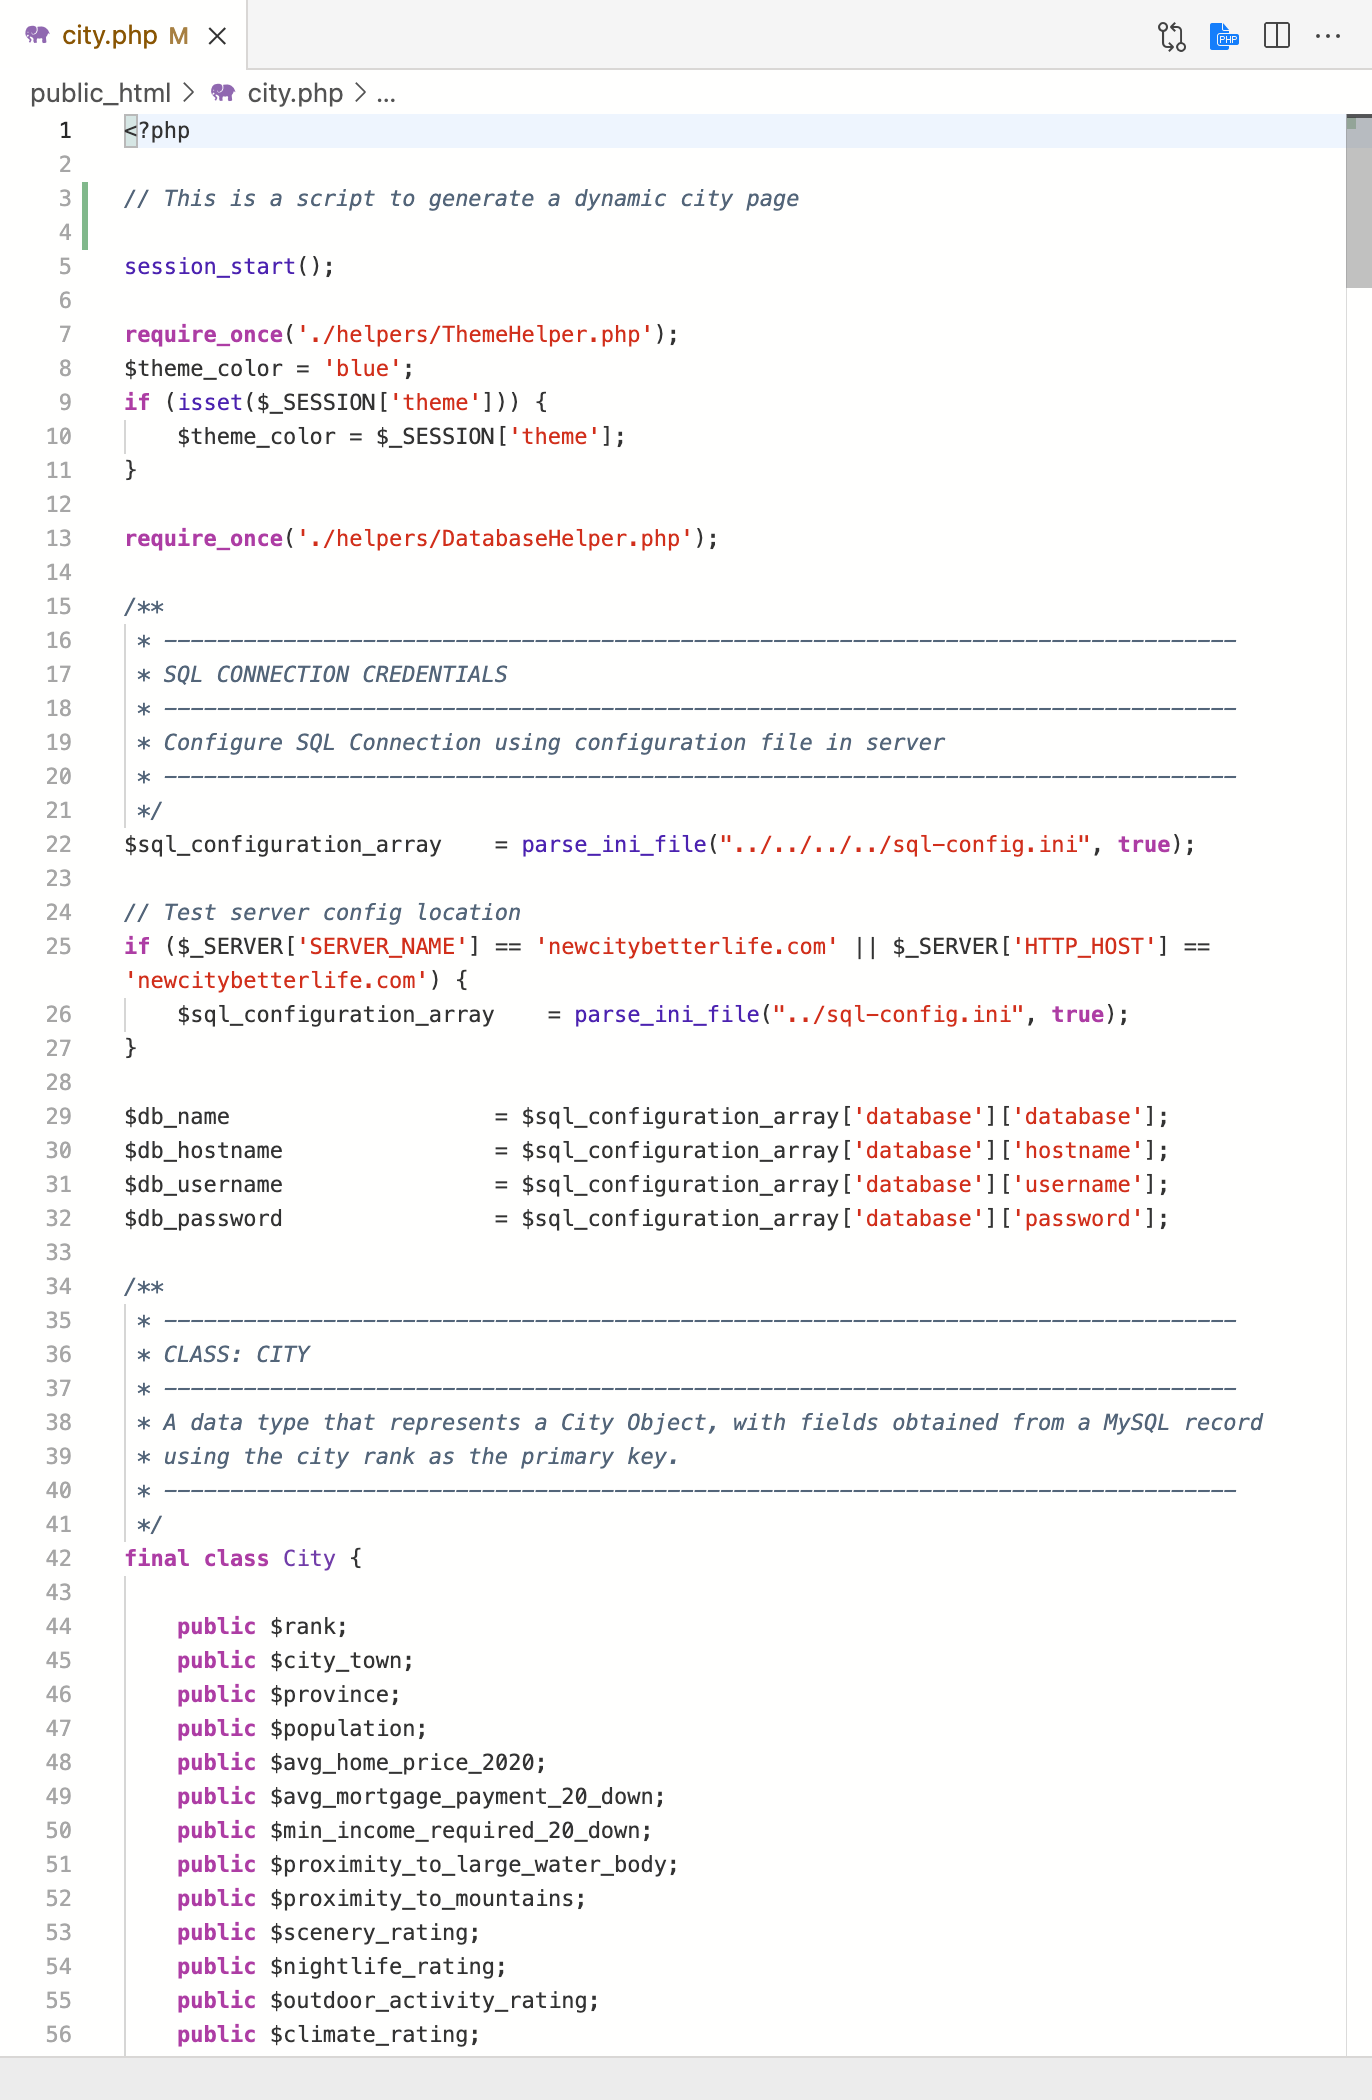
\includegraphics[width=4.3in]{images/22-script-1.png}
	\caption{Script: city.php}
 \end{figure}

 
%   Script 2
% ------------------------------------------------------------------------

\begin{figure}[htbp]
	\centering
	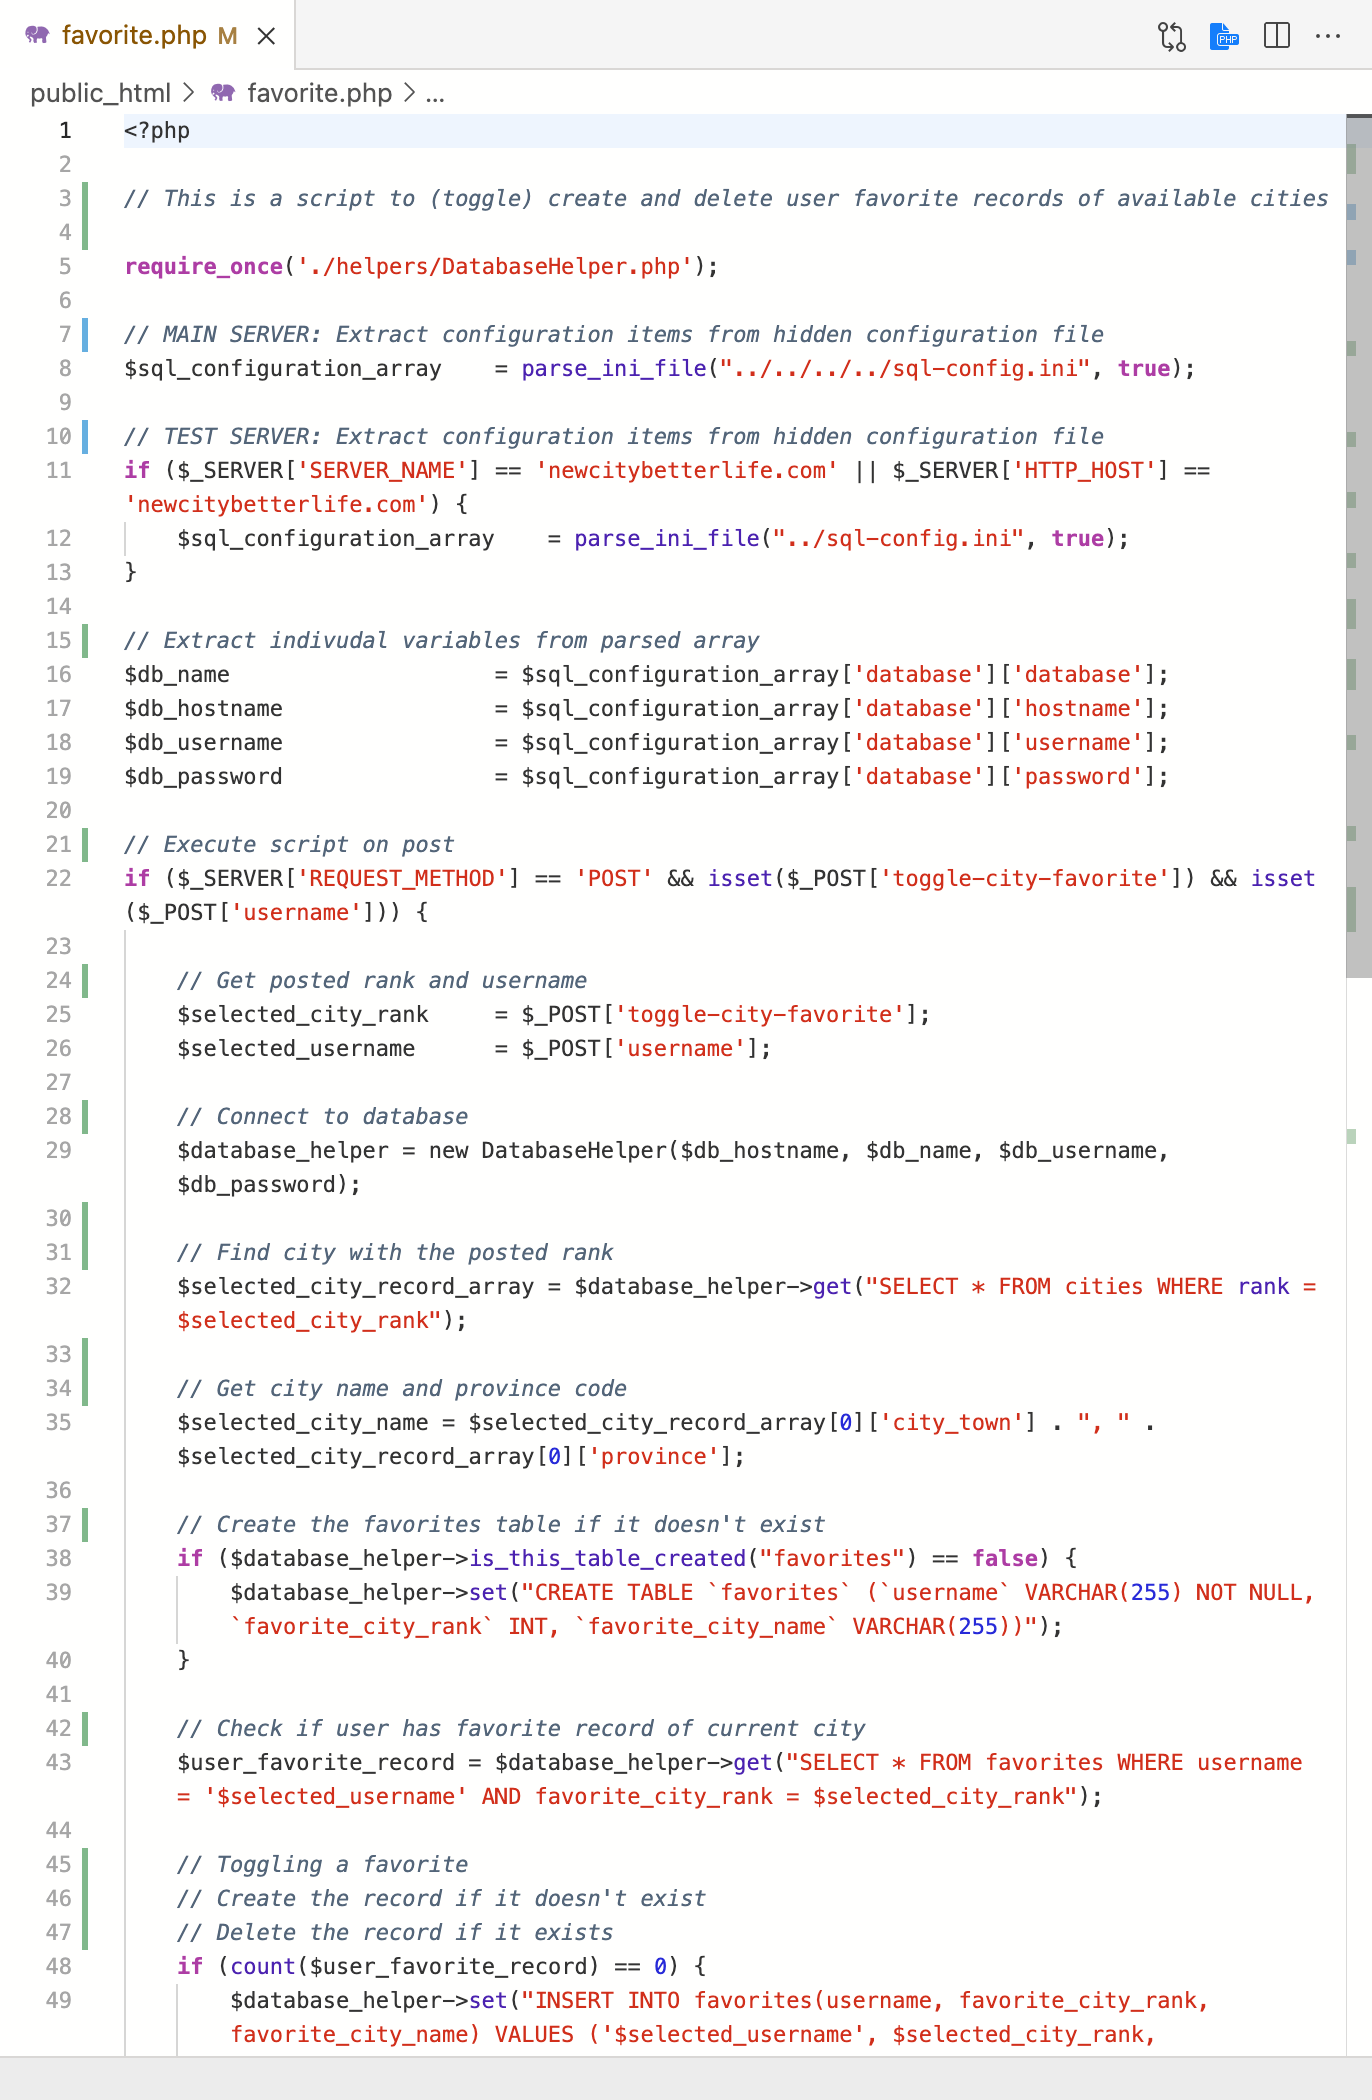
\includegraphics[width=4.3in]{images/22-script-2.png}
	\caption{Script: favorite.php}
 \end{figure}

%   Script 3
% ------------------------------------------------------------------------

\begin{figure}[htbp]
	\centering
	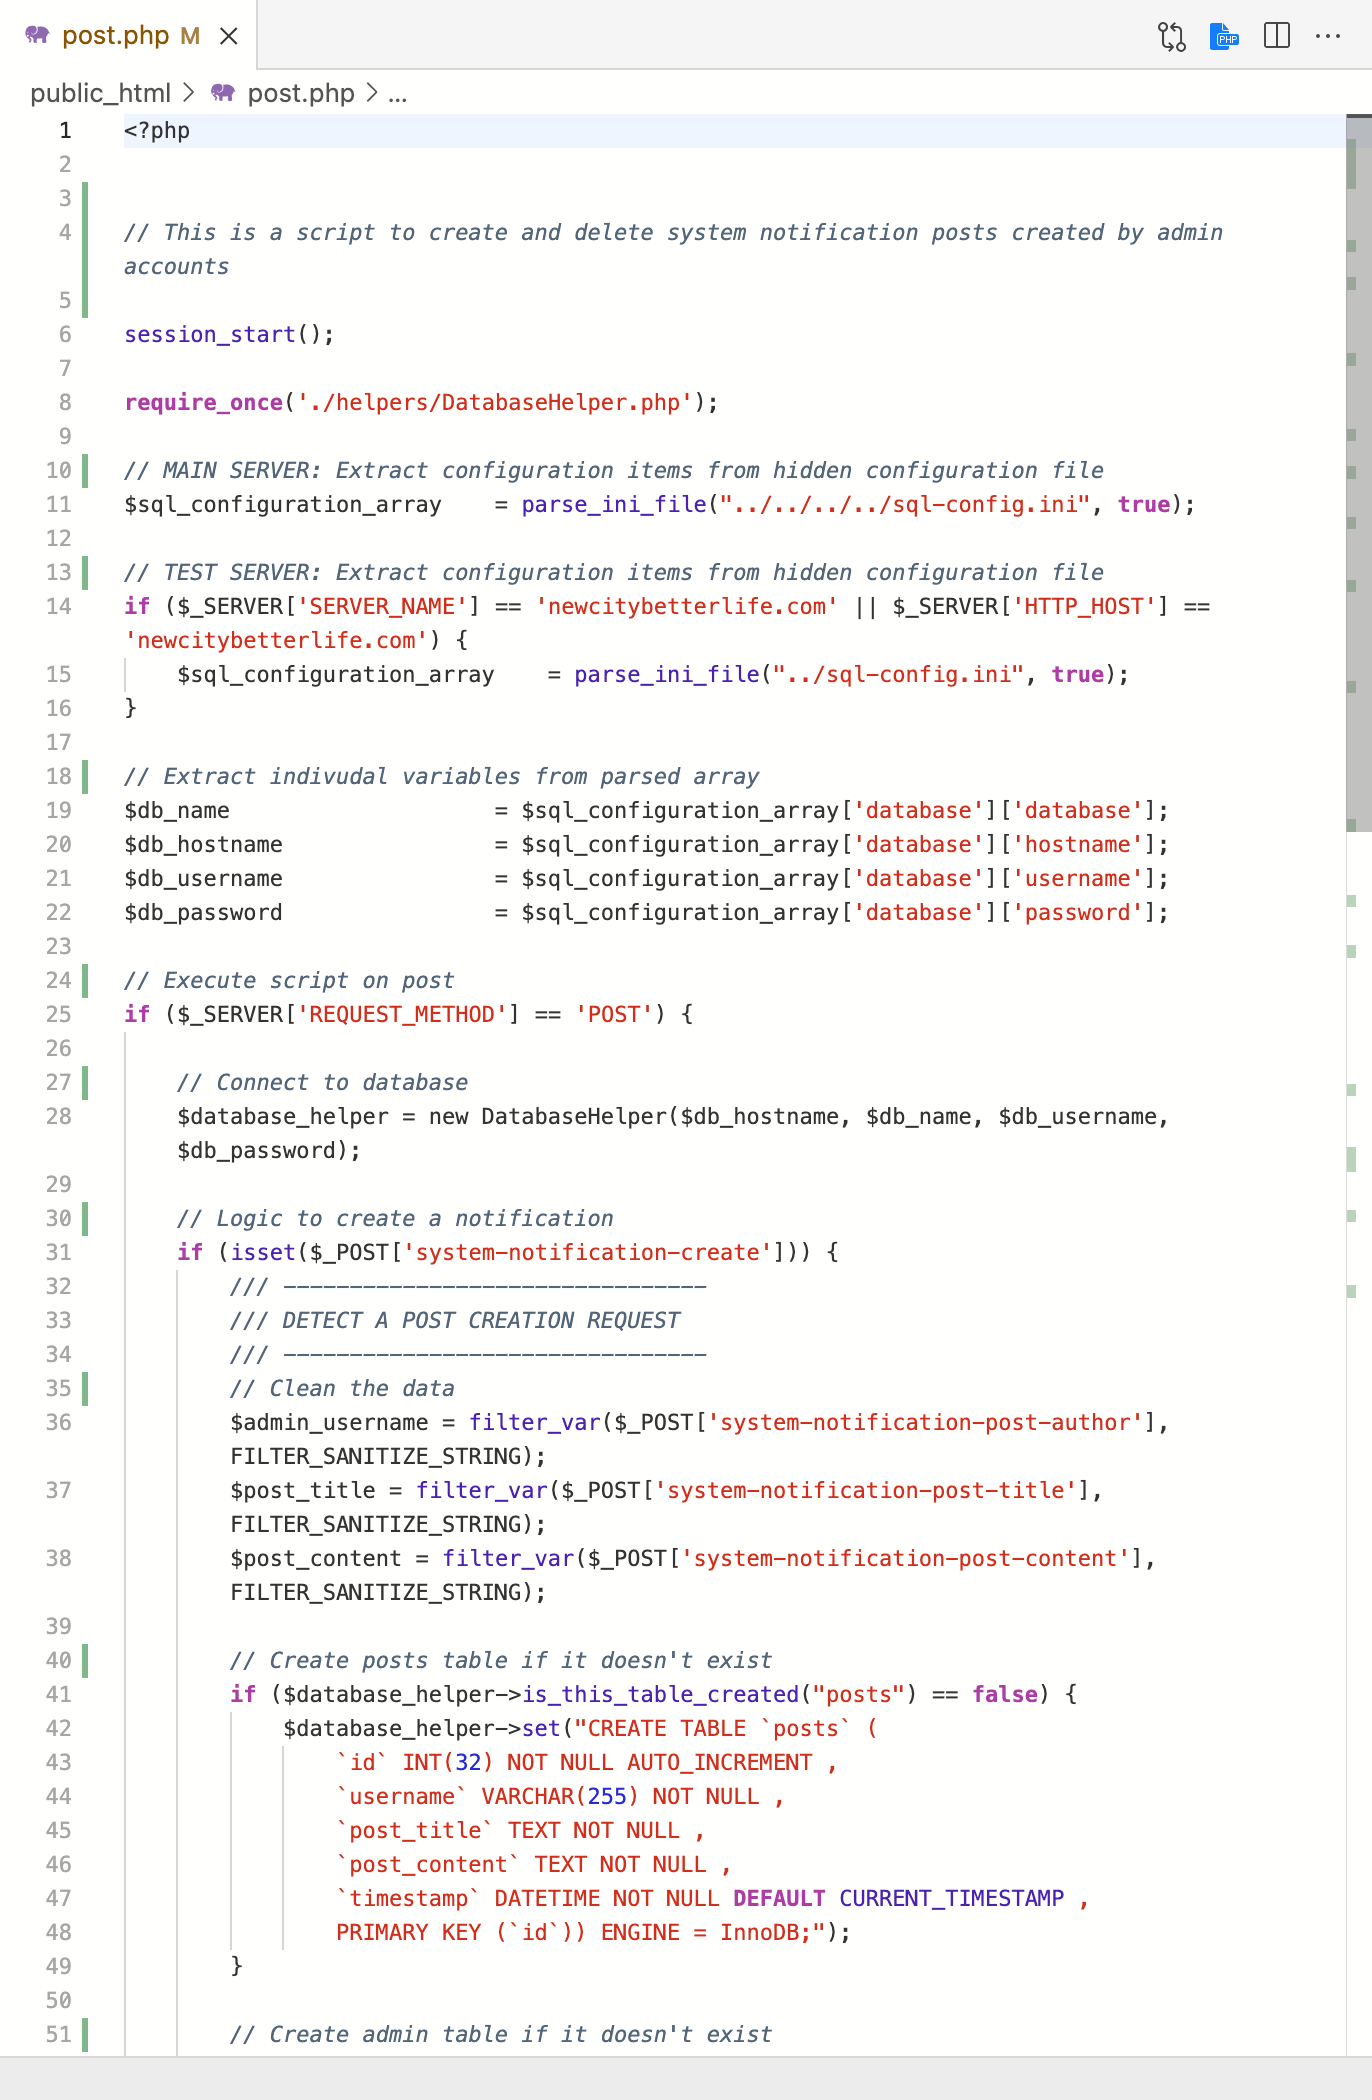
\includegraphics[width=4.3in]{images/22-script-3.png}
	\caption{Script: post.php}
 \end{figure}

%   Script 4
% ------------------------------------------------------------------------

\begin{figure}[htbp]
	\centering
	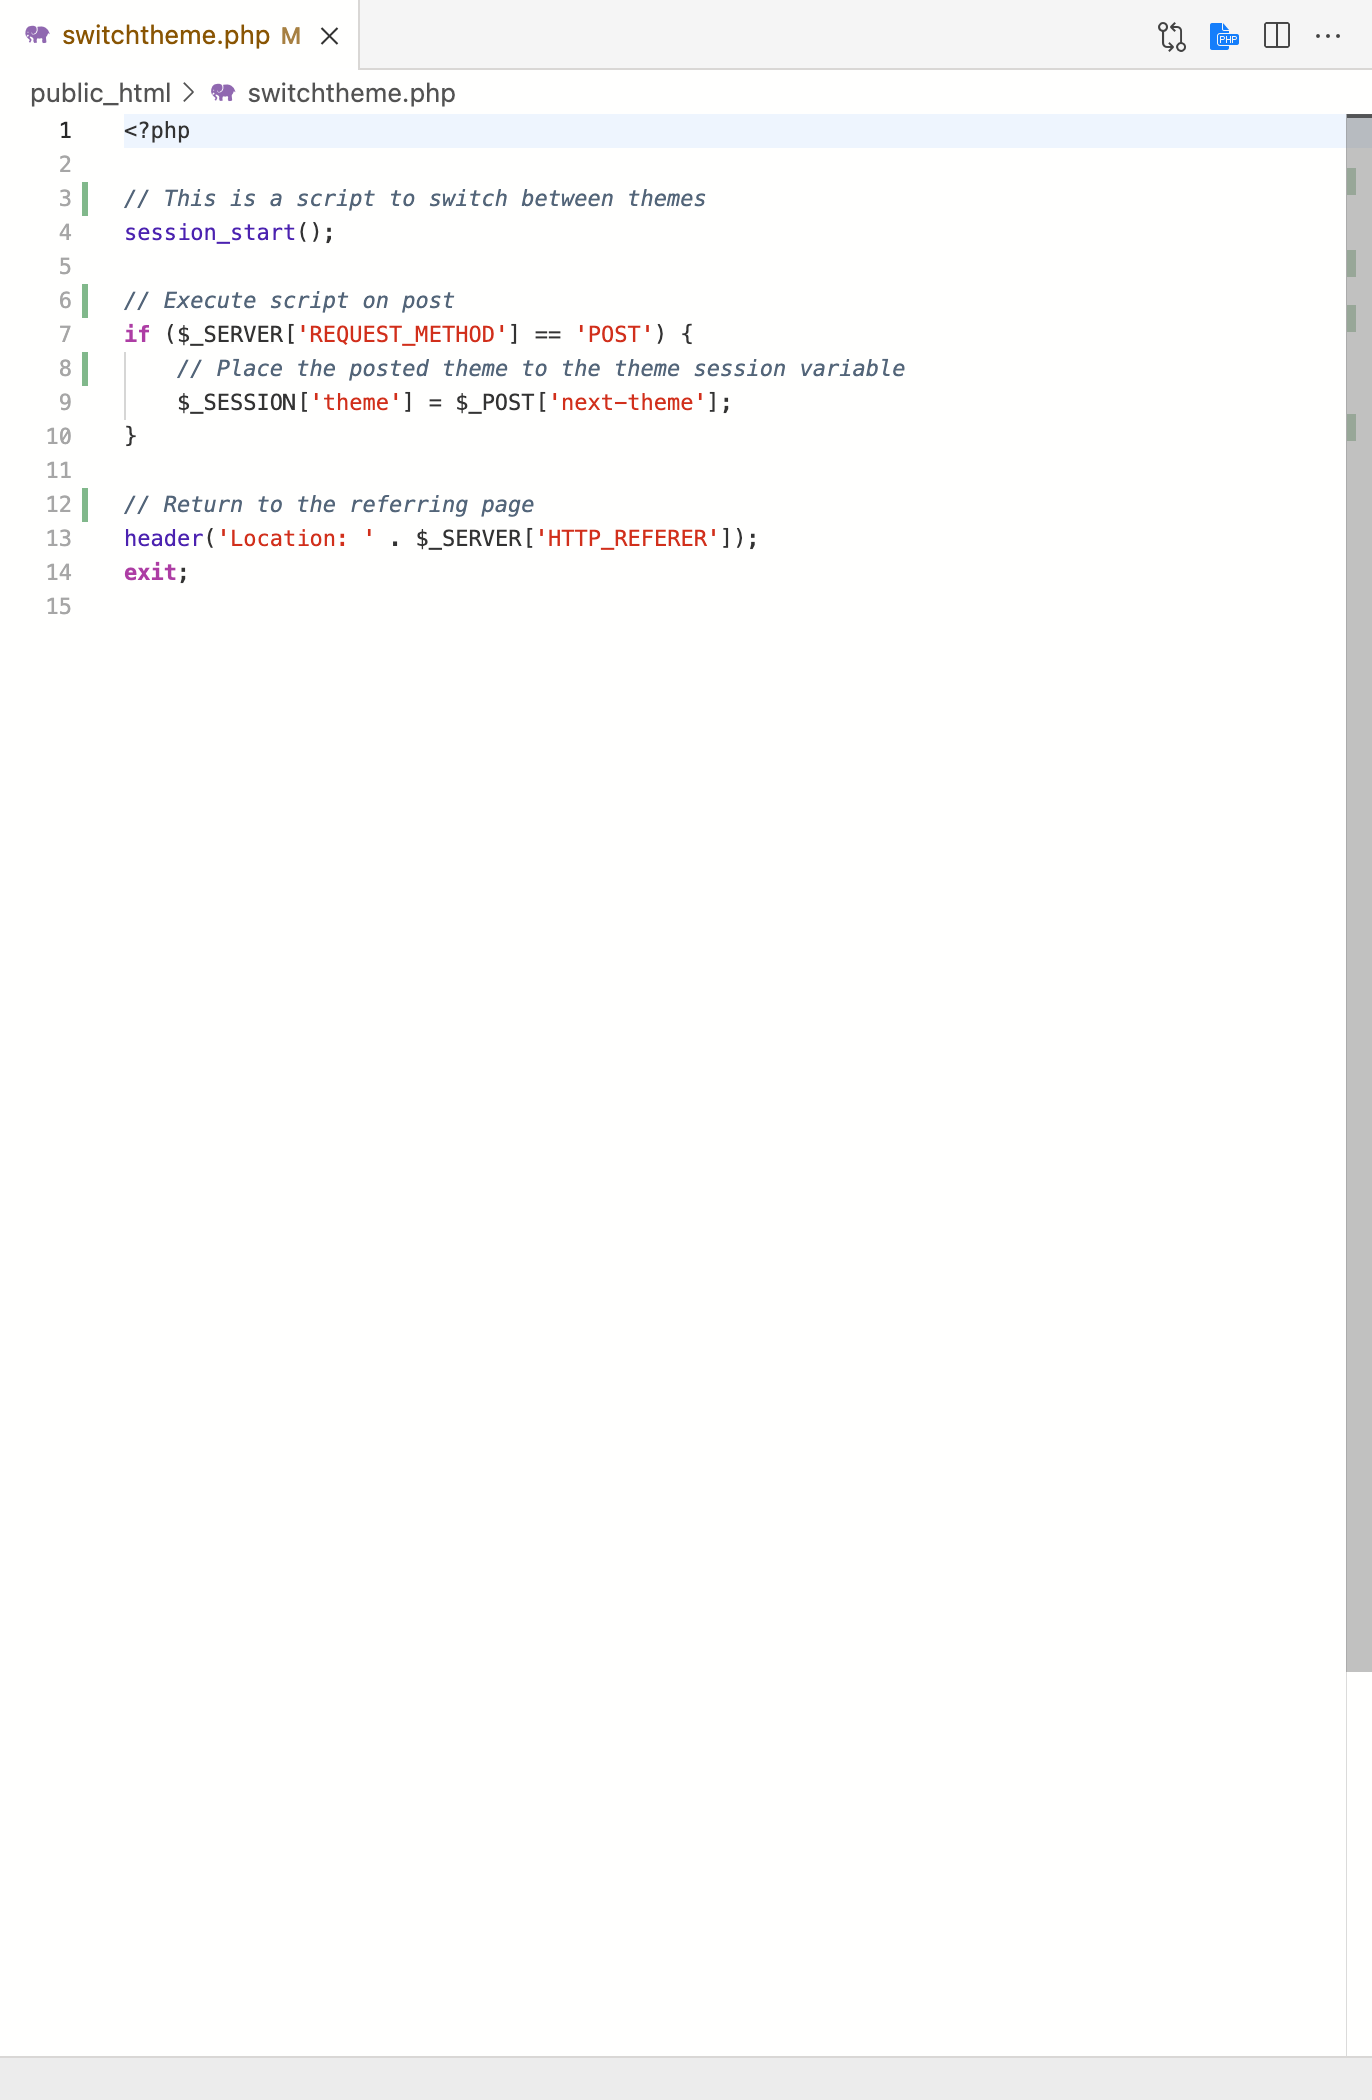
\includegraphics[width=4.3in]{images/22-script-4.png}
	\caption{Script: switchtheme.php}
 \end{figure}

%   Script 5
% ------------------------------------------------------------------------

\begin{figure}[htbp]
	\centering
	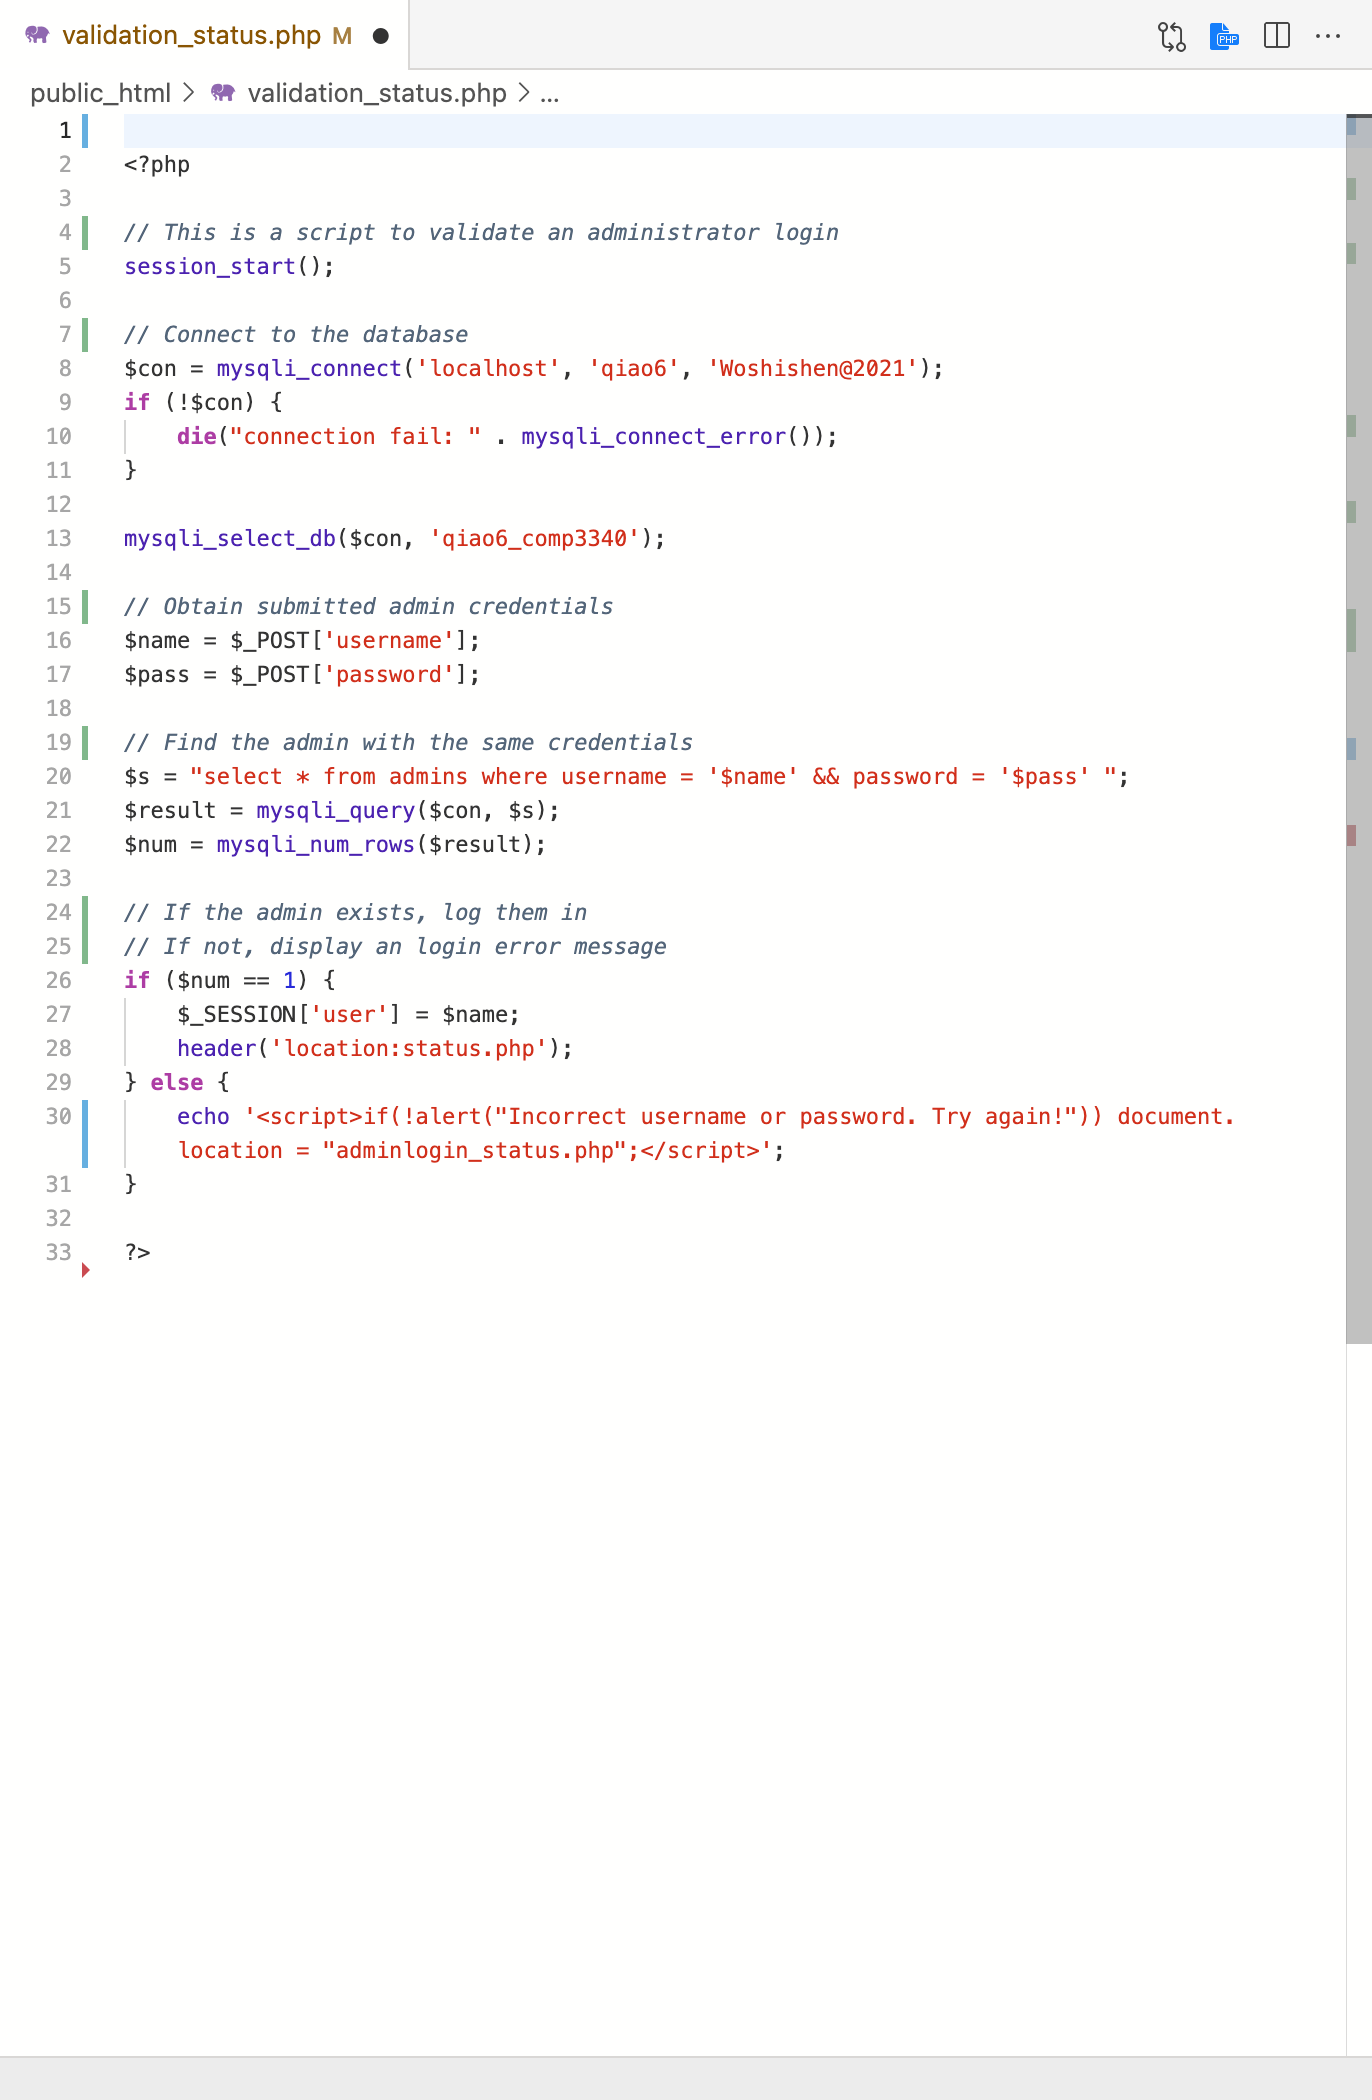
\includegraphics[width=4.3in]{images/22-script-5.png}
	\caption{Script: validation\_status.php}
 \end{figure}

 \newpage

% =====================================================================
%   23. ADDITIONAL LANGUAGE / FRAMEWORK
% =====================================================================
\section{Additional Language/Framework}
For our project, we used two additional frameworks. 

\subsection*{PlotlyJS}
The first framework is PlotlyJS, which is a graphing framework used to visualize our dataset. The framework provides an ability for developers to create interactive graphs and data visualizations from inputted data.
\begin{figure}[htbp]
	\centering
	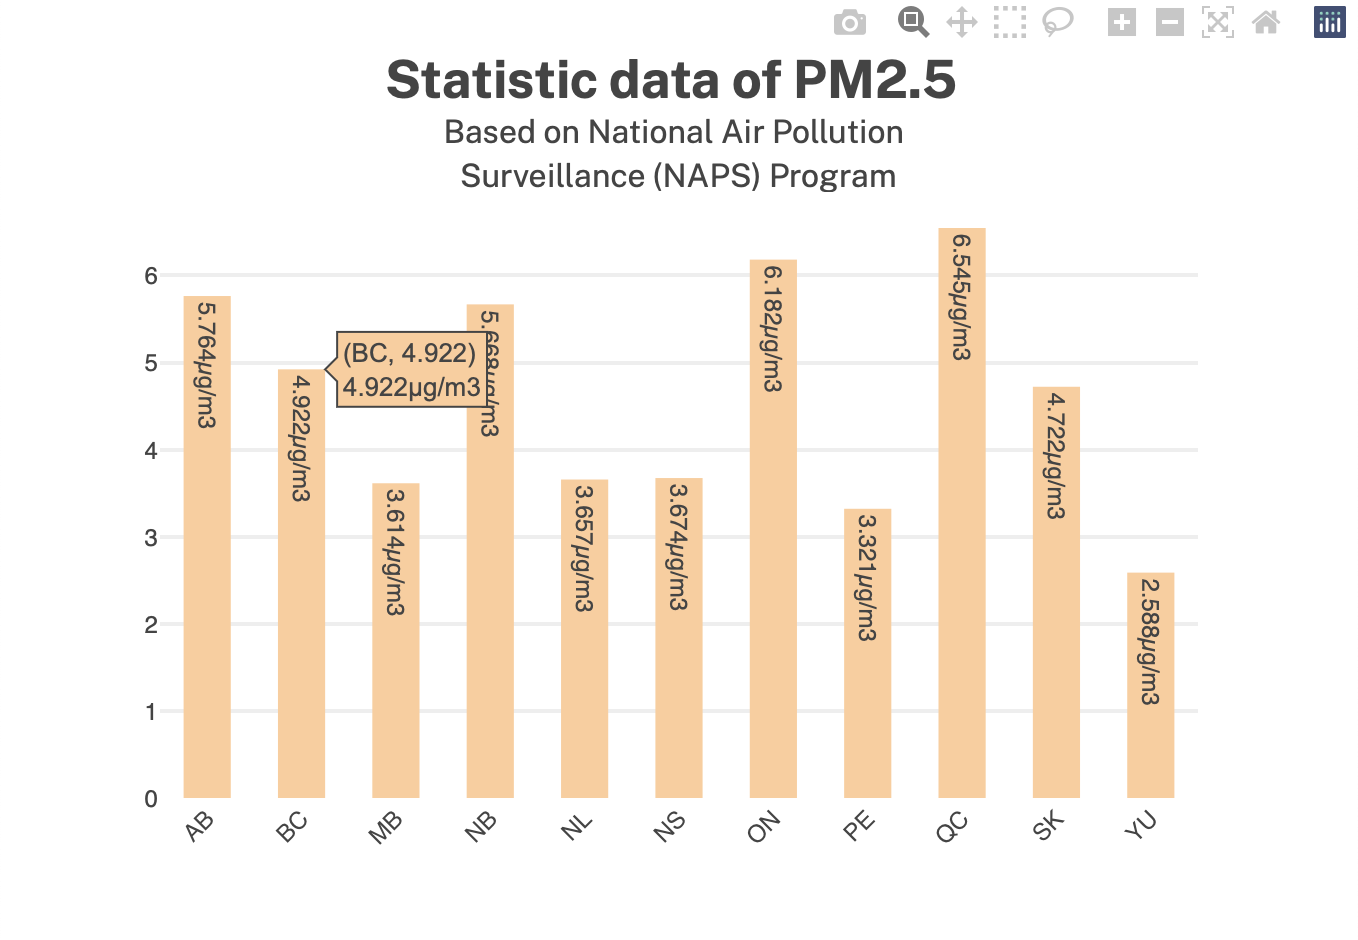
\includegraphics[width=\textwidth]{images/23-plotlyjs.png}
	\caption{Framework 1: PlotlyJS}
 \end{figure}

\newpage
 \subsection*{Bootstrap}
 The second framework is Bootstrap, which was used to design key pages for the website, while also making these pages responsive. The framework provides the ability for developers to create and style elements using pre-designed css elements that are part of the bootstrap framework.
 \begin{figure}[htbp]
	\centering
	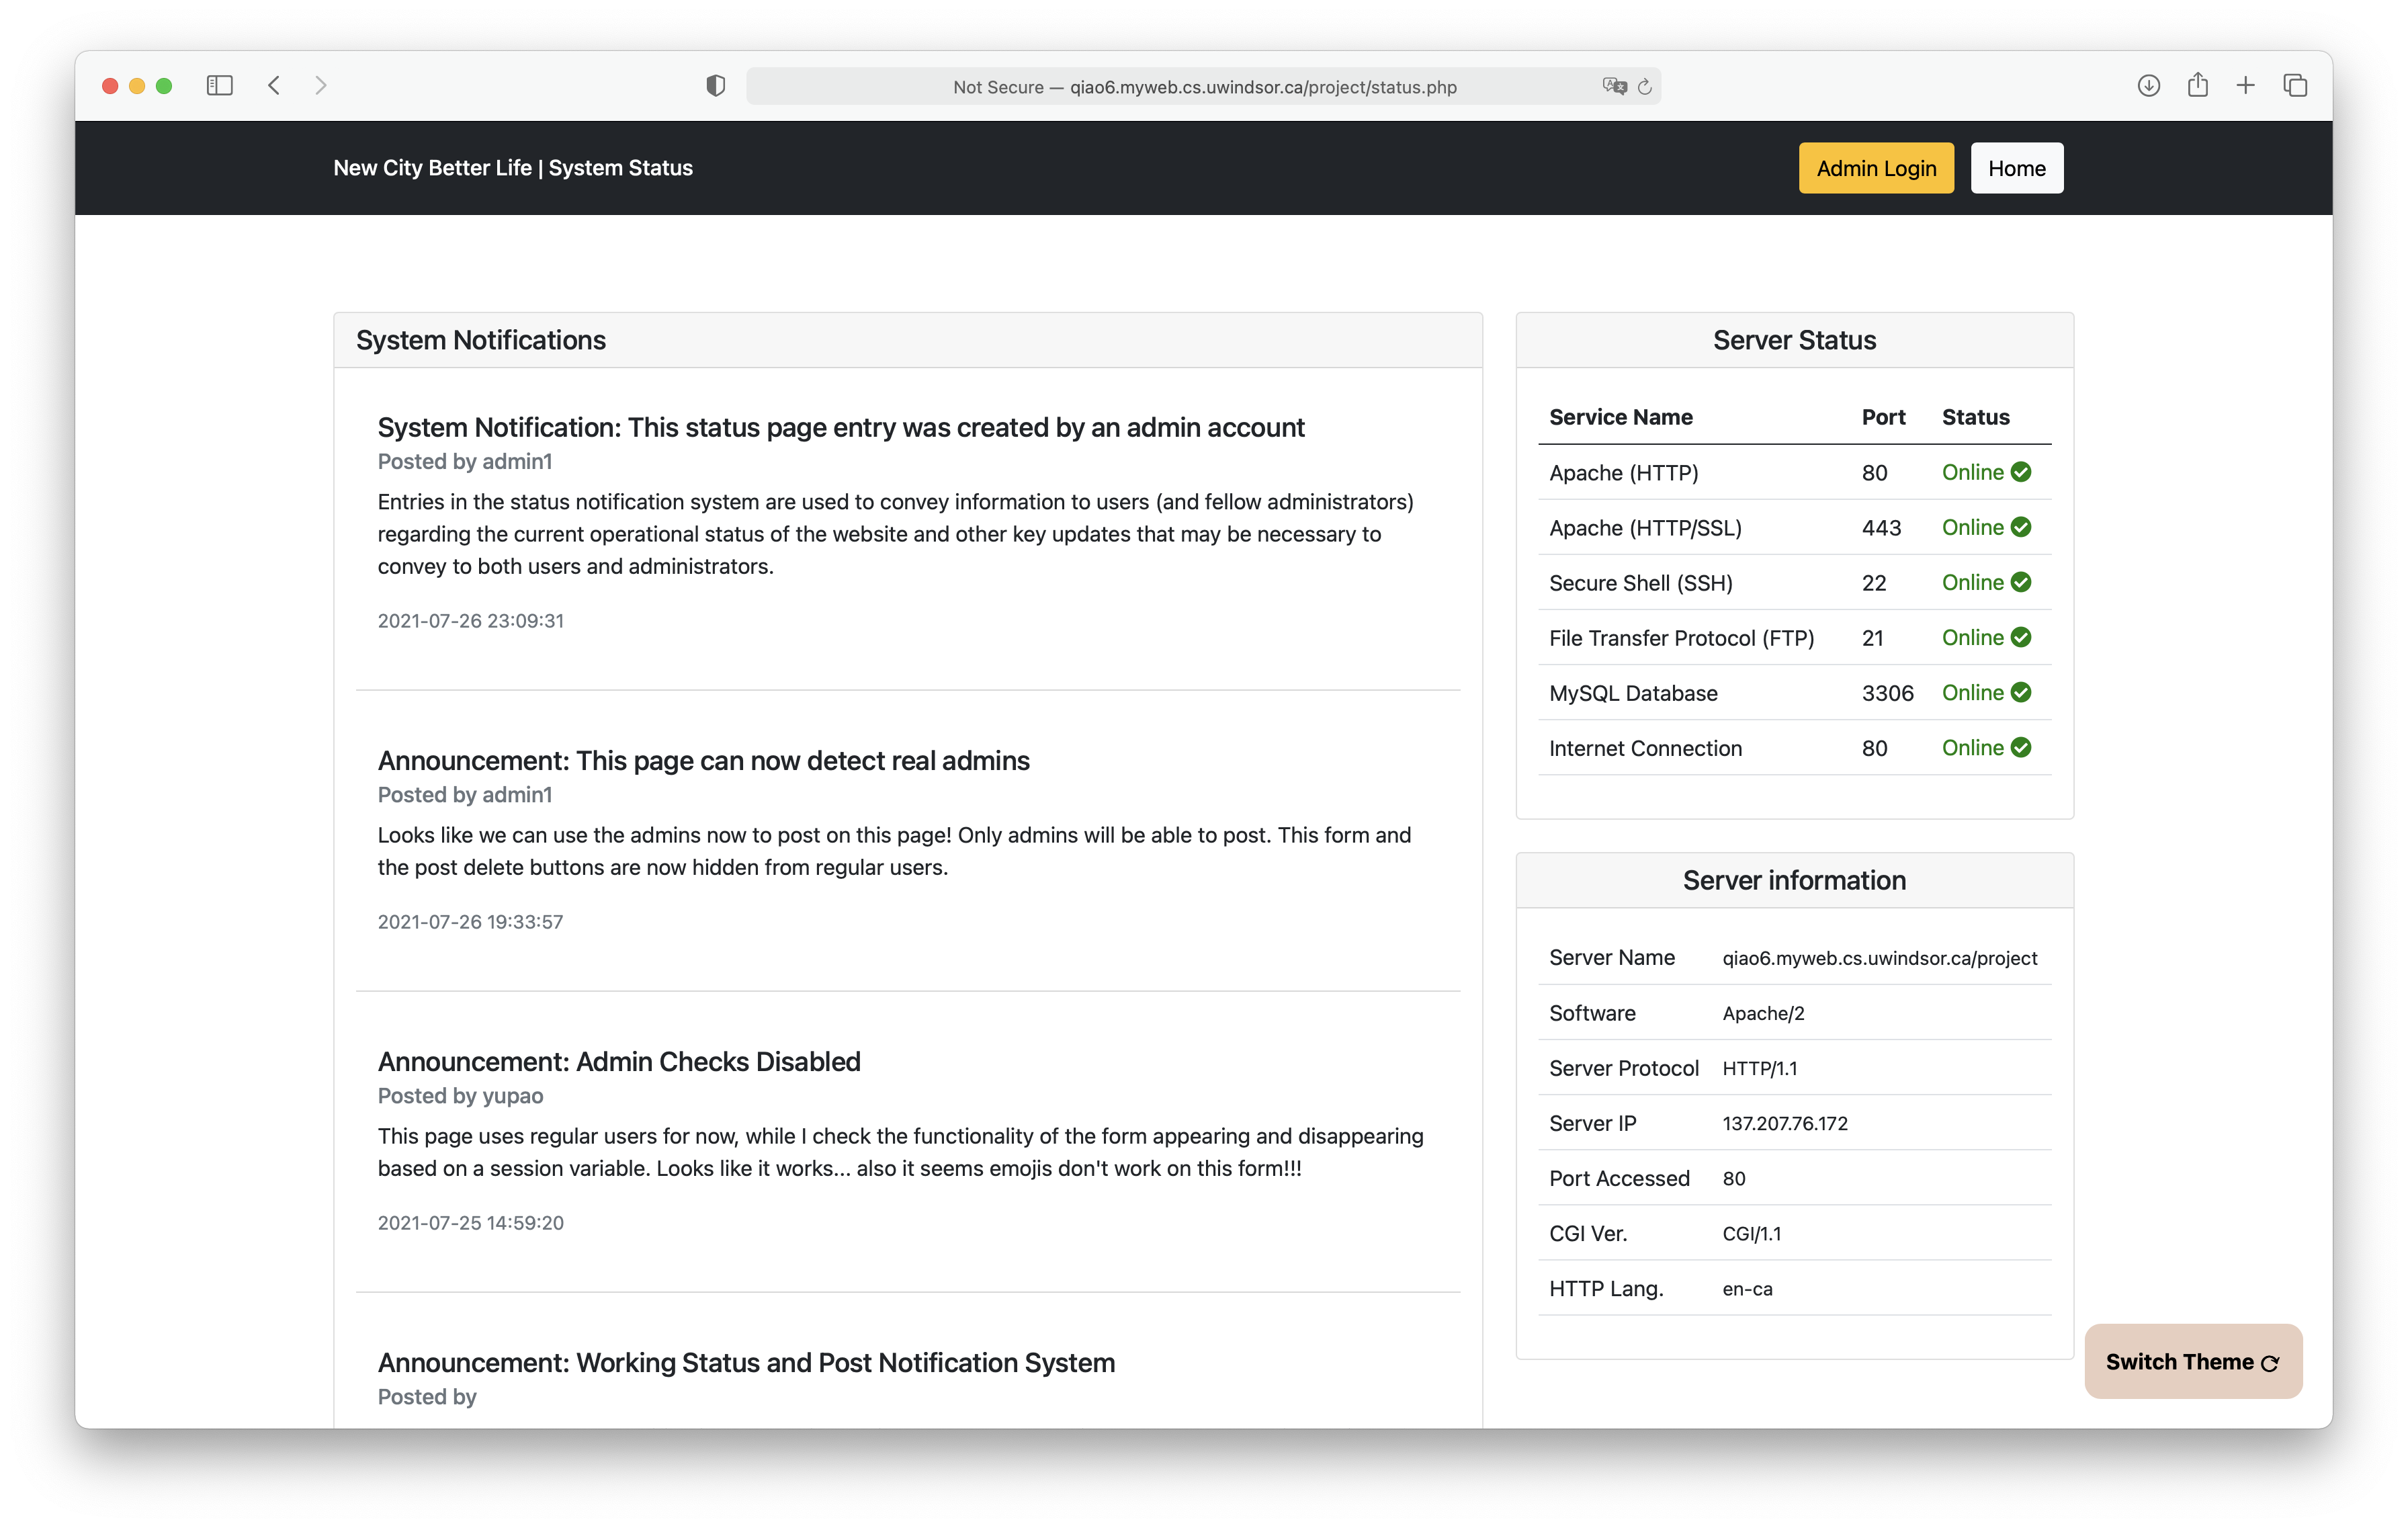
\includegraphics[width=\textwidth]{images/23-bootstrap.png}
	\caption{Framework 2: Bootstrap}
 \end{figure}

 \newpage

% =====================================================================
%   24. SOFTWARE REPOSITORY
% =====================================================================
\section{Software Repository}
We used GitHub to host our official repository. The repository can be found at \url{https://github.com/ChenQiao310/Project-COMP3340}. 

\subsection*{Open-Source Access}
The repository is currently public and open-source, which means it is open to all users for cloning, forking and also contributing through fork pull requests (but not direct push access).

\begin{figure}[htbp]
	\centering
	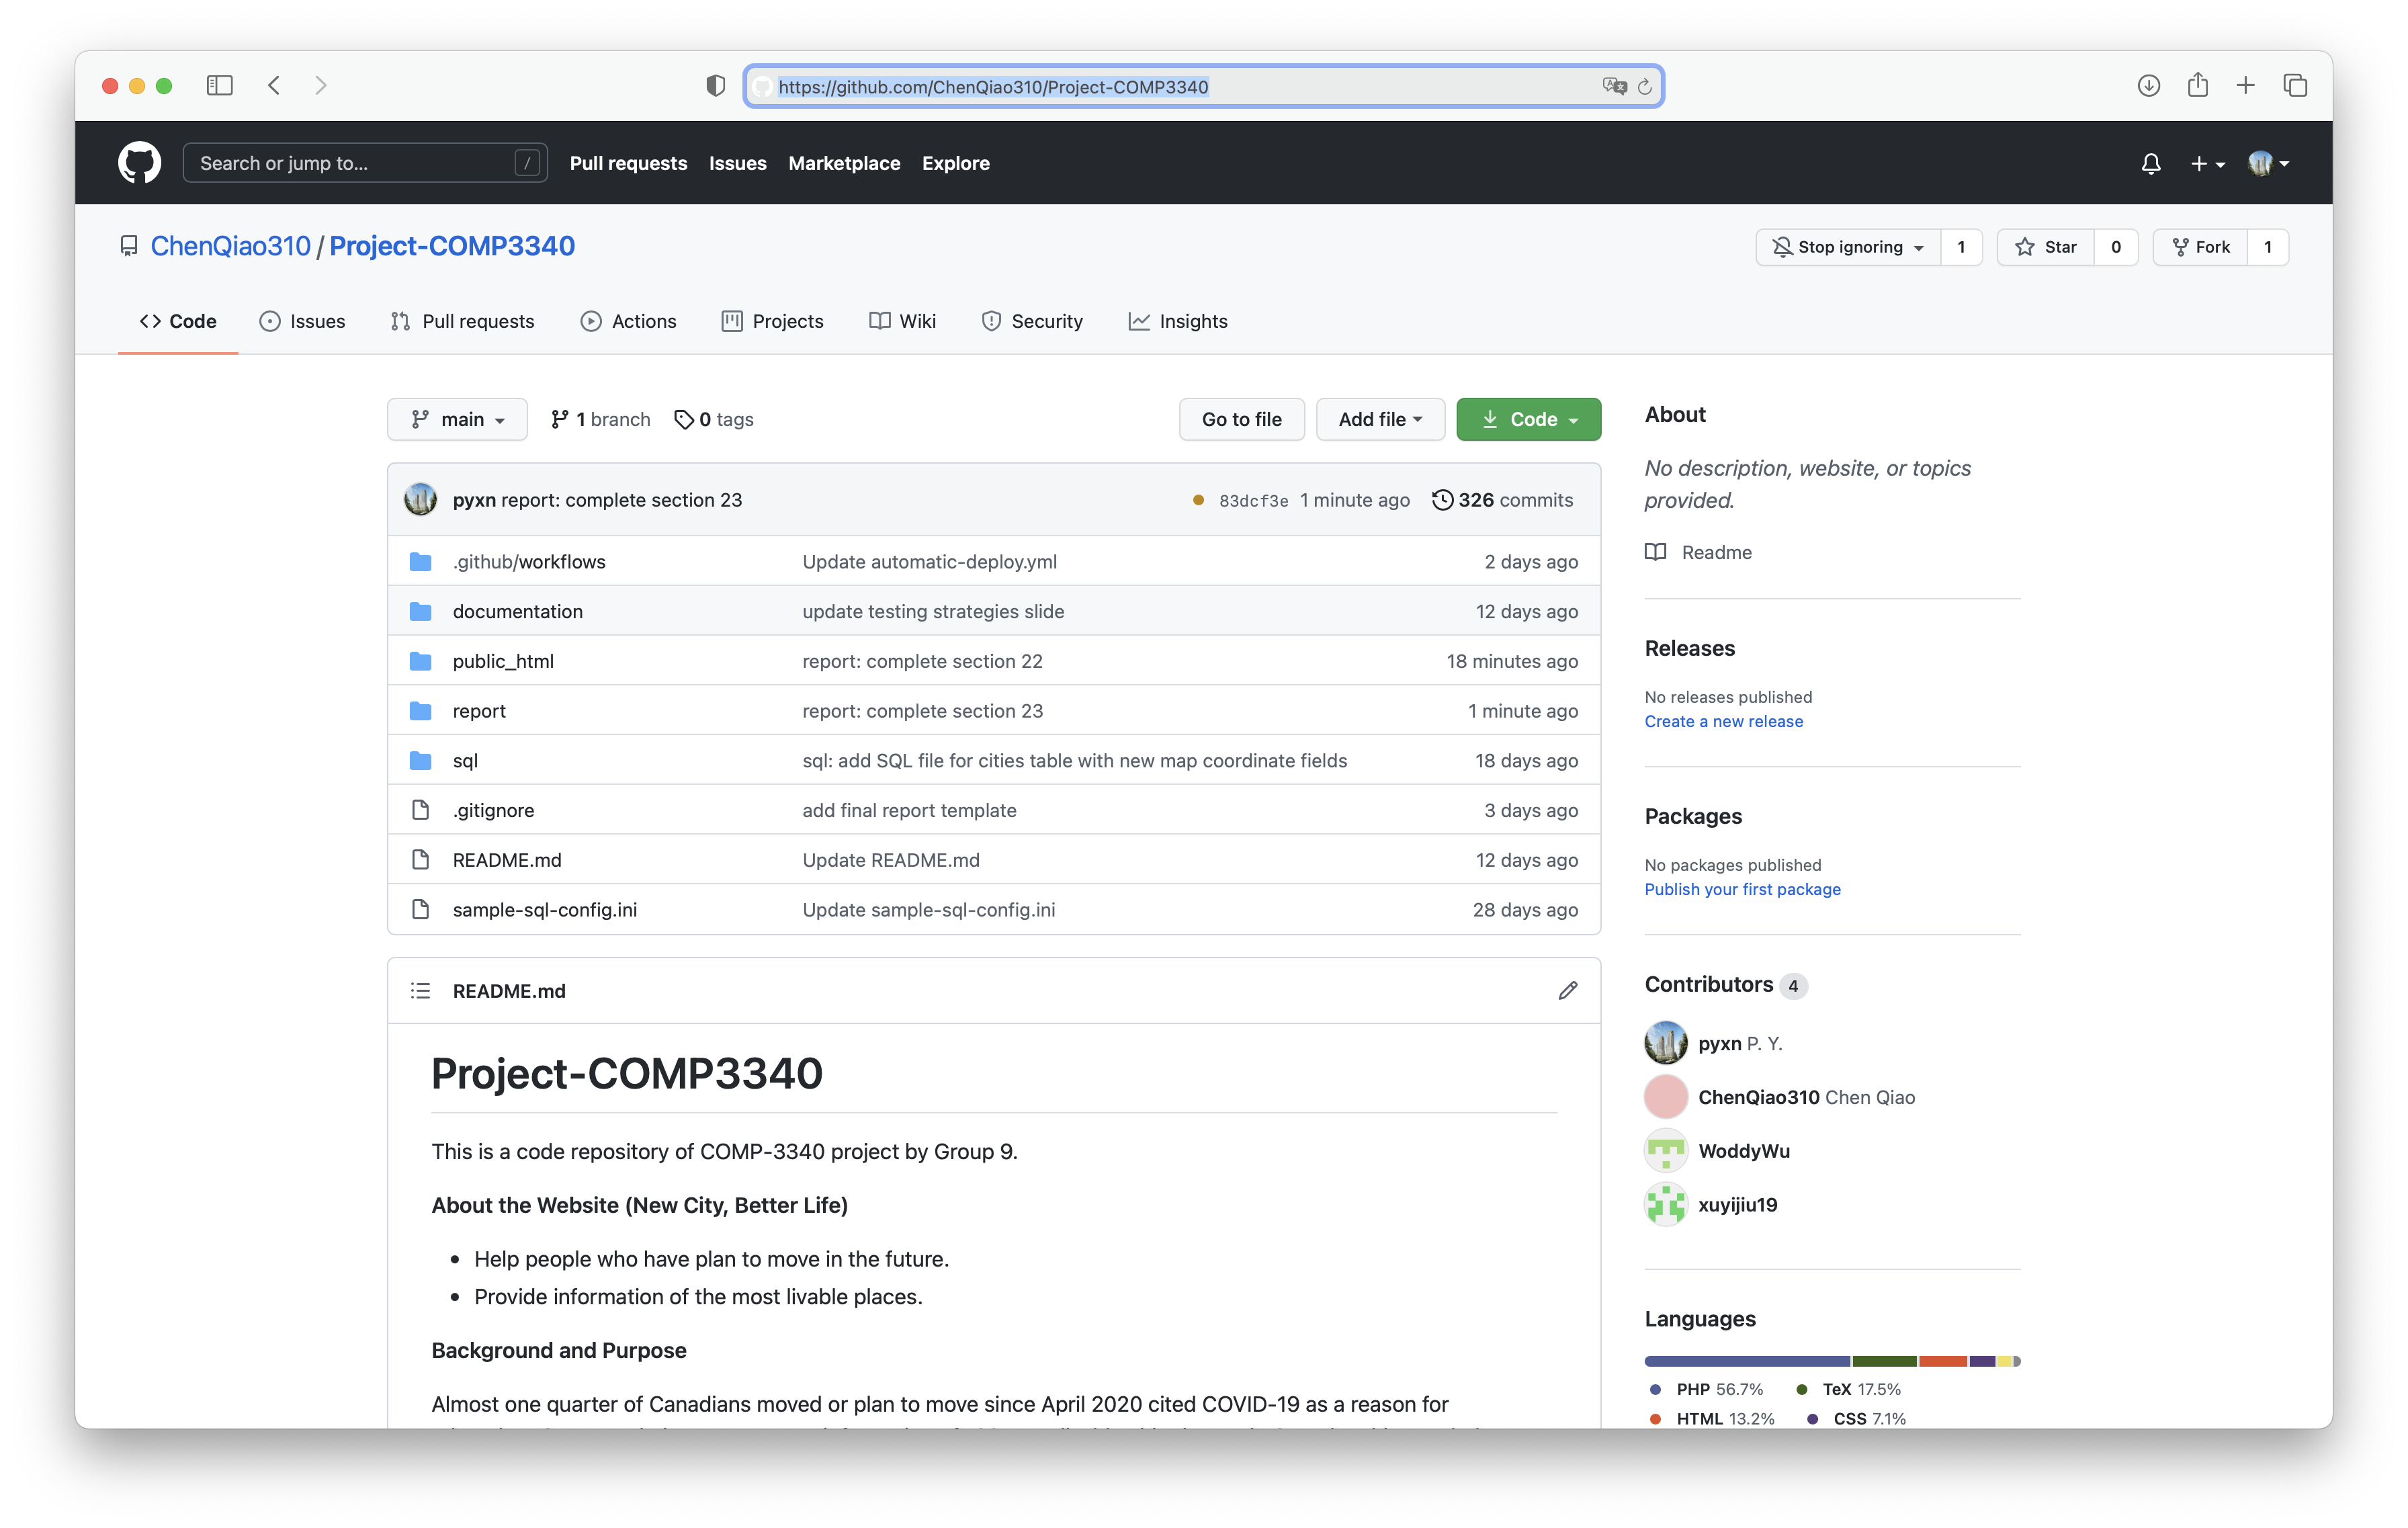
\includegraphics[width=\textwidth]{images/24-repo.png}
	\caption{Official Repository on GitHub}
 \end{figure}

 \newpage

% =====================================================================
%   25. INSTALLATION AND DEPLOYMENT
% =====================================================================
\section{Installation and Deployment}

\subsection*{Open-Source Access}
Since the project's repository is currently public and open-source, the site can be cloned, downloaded, or forked by any third party. The parameters for the database and other website elements themselves can be modified by the third-party developers.

\subsection*{Official Release Download}
Alternatively, developers can download the official release packages, such as the one displayed below. These releases can be accessed through the open-source repository.

\begin{figure}[htbp]
	\centering
	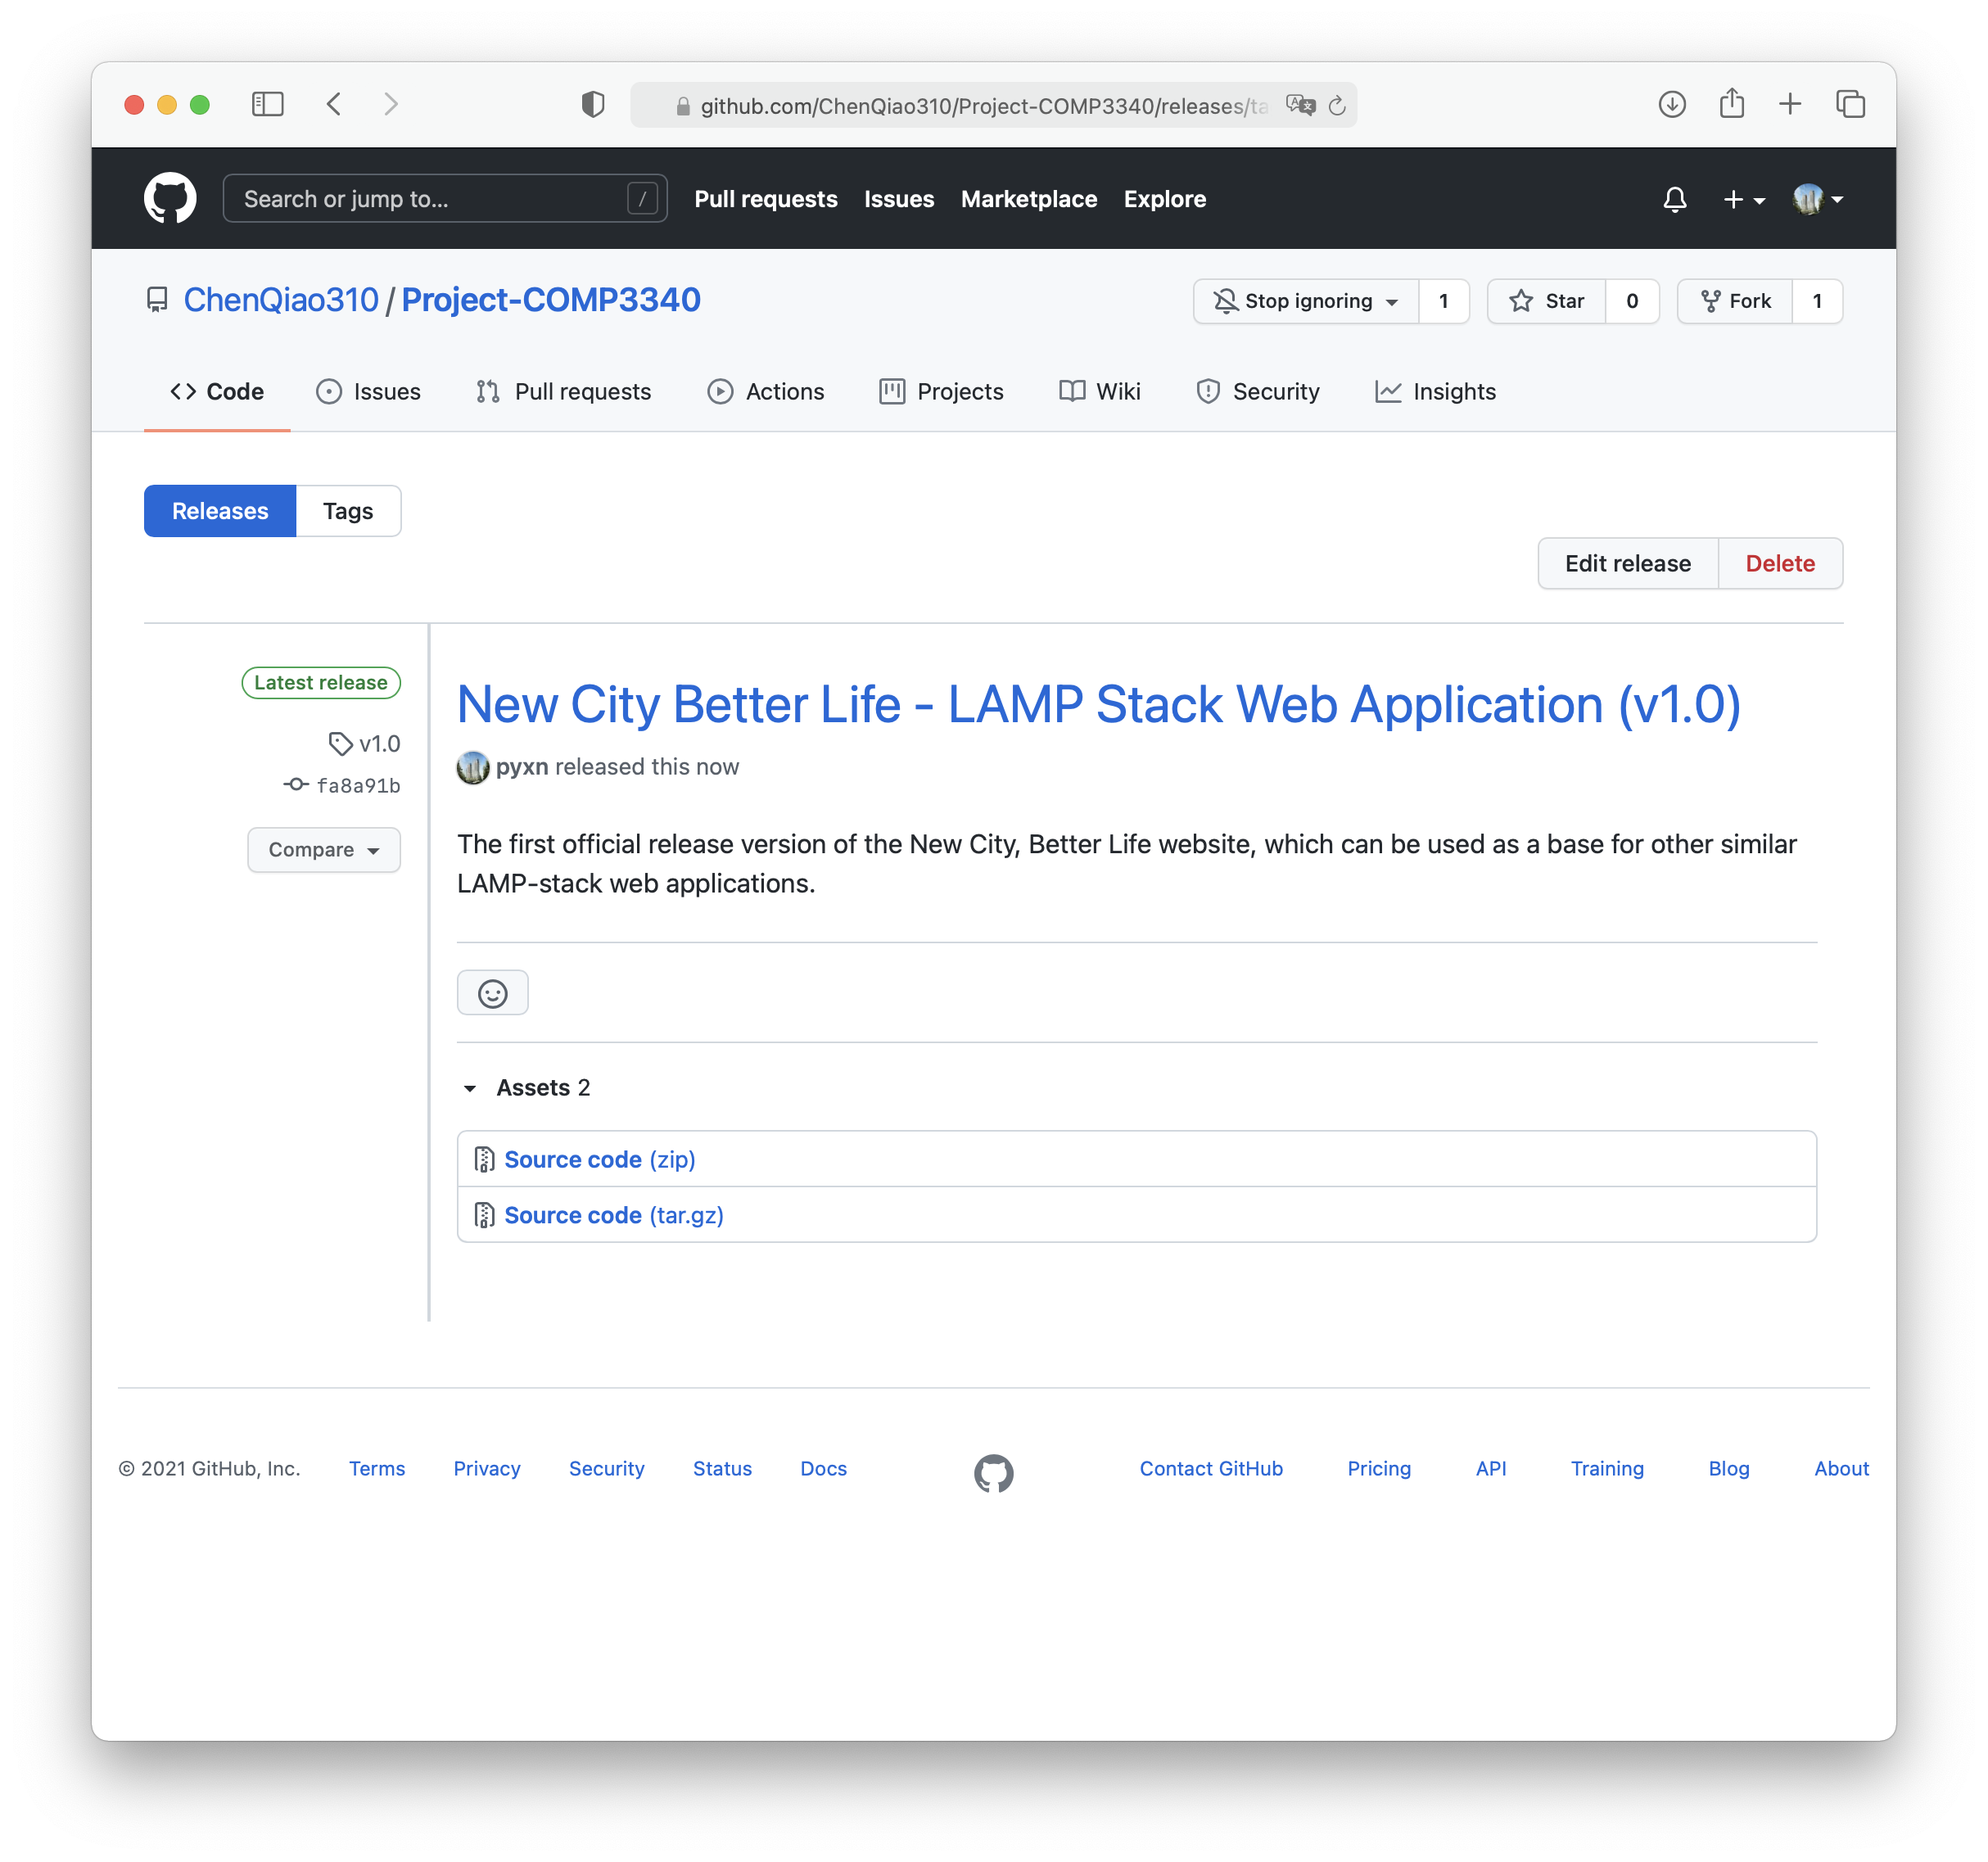
\includegraphics[width=\textwidth]{images/25-release.png}
	\caption{New City, Better Life Official Release}
 \end{figure}

\subsection*{Installation and Deployment}
Once the project is cloned or forked into the third-pary developer's account, it can then be installed and deployed using our proprietary deployment tool, \lstinline{SFTP-Mirror}. It is a custom continous integration tool that can be used to instantly deploy any web-based project to a server from any GitHub repository. The custom deployment tool can be accessed at \url{https://github.com/pyxn/sftp-mirror}

\begin{figure}[htbp]
	\centering
	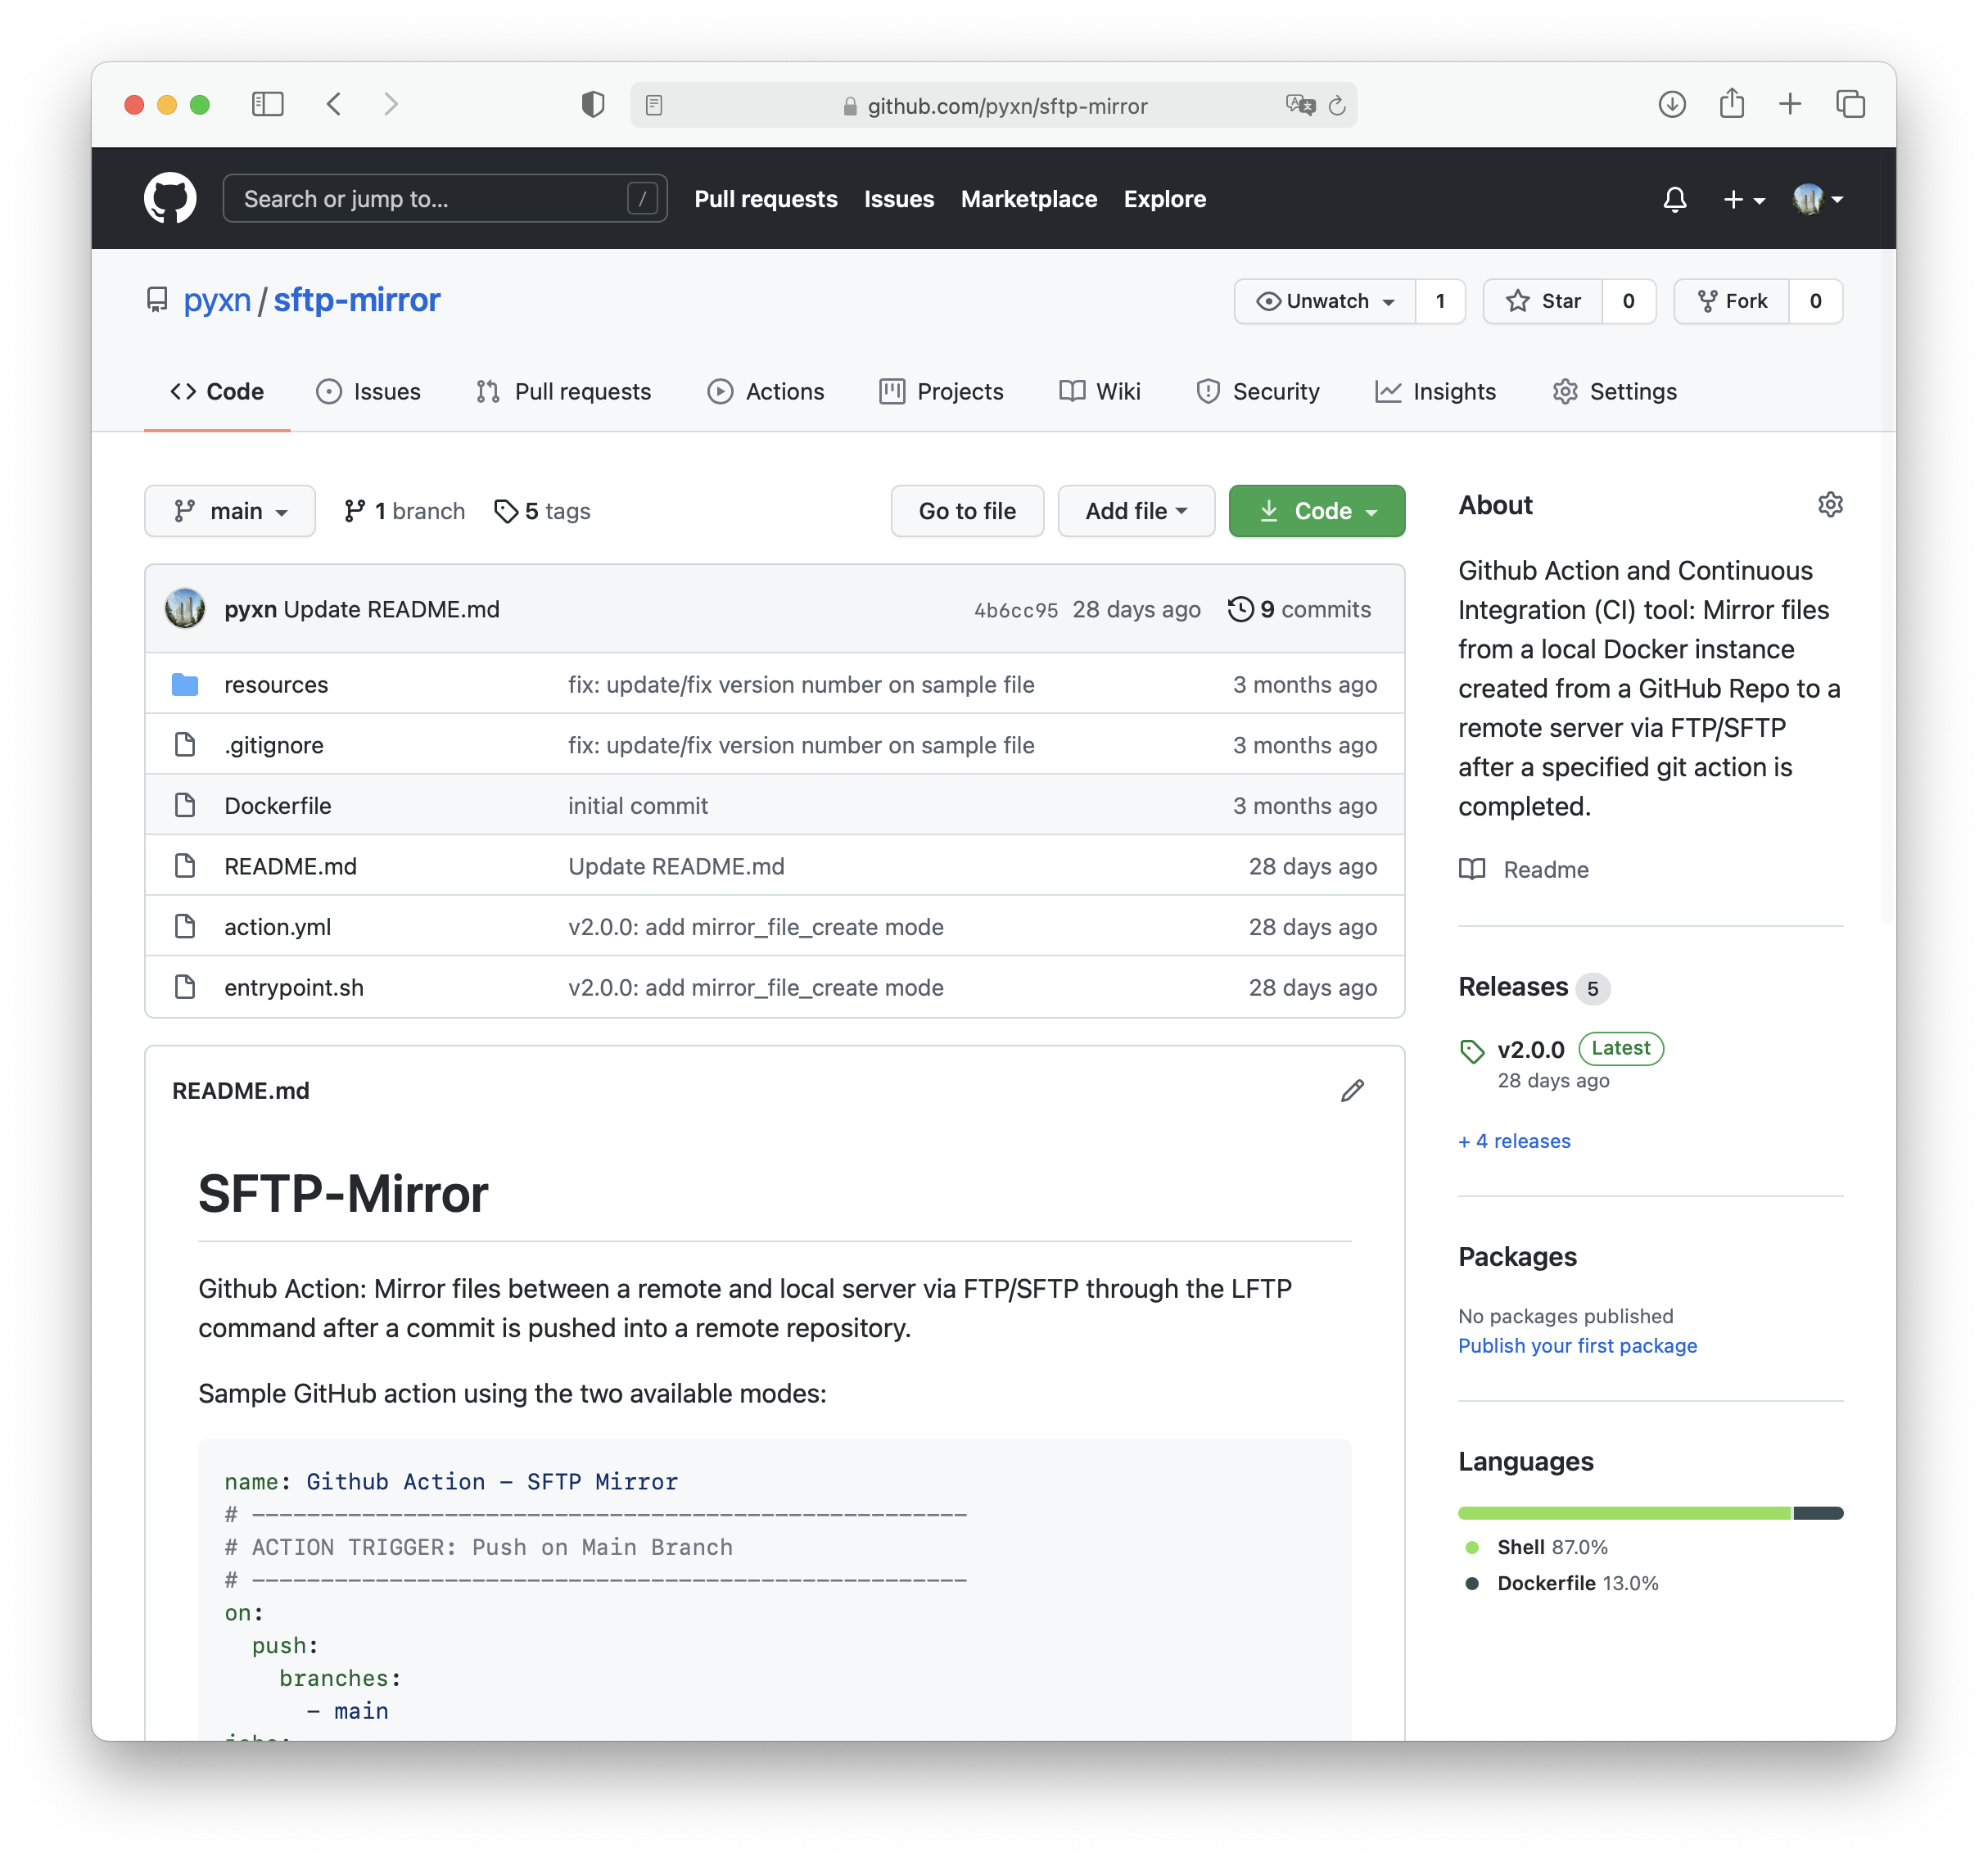
\includegraphics[width=\textwidth]{images/25-sftp-mirror.png}
	\caption{SFTP-Mirror: Custom Deployment Tool}
 \end{figure}

\newpage
\subsection*{Usage}
The tool's usage and implementation details can be accessed through the official instructions and readme file in the \lstinline{SFTP-Mirror} repository (\url{https://github.com/pyxn/sftp-mirror/blob/main/README.md})

\begin{figure}[htbp]
	\centering
	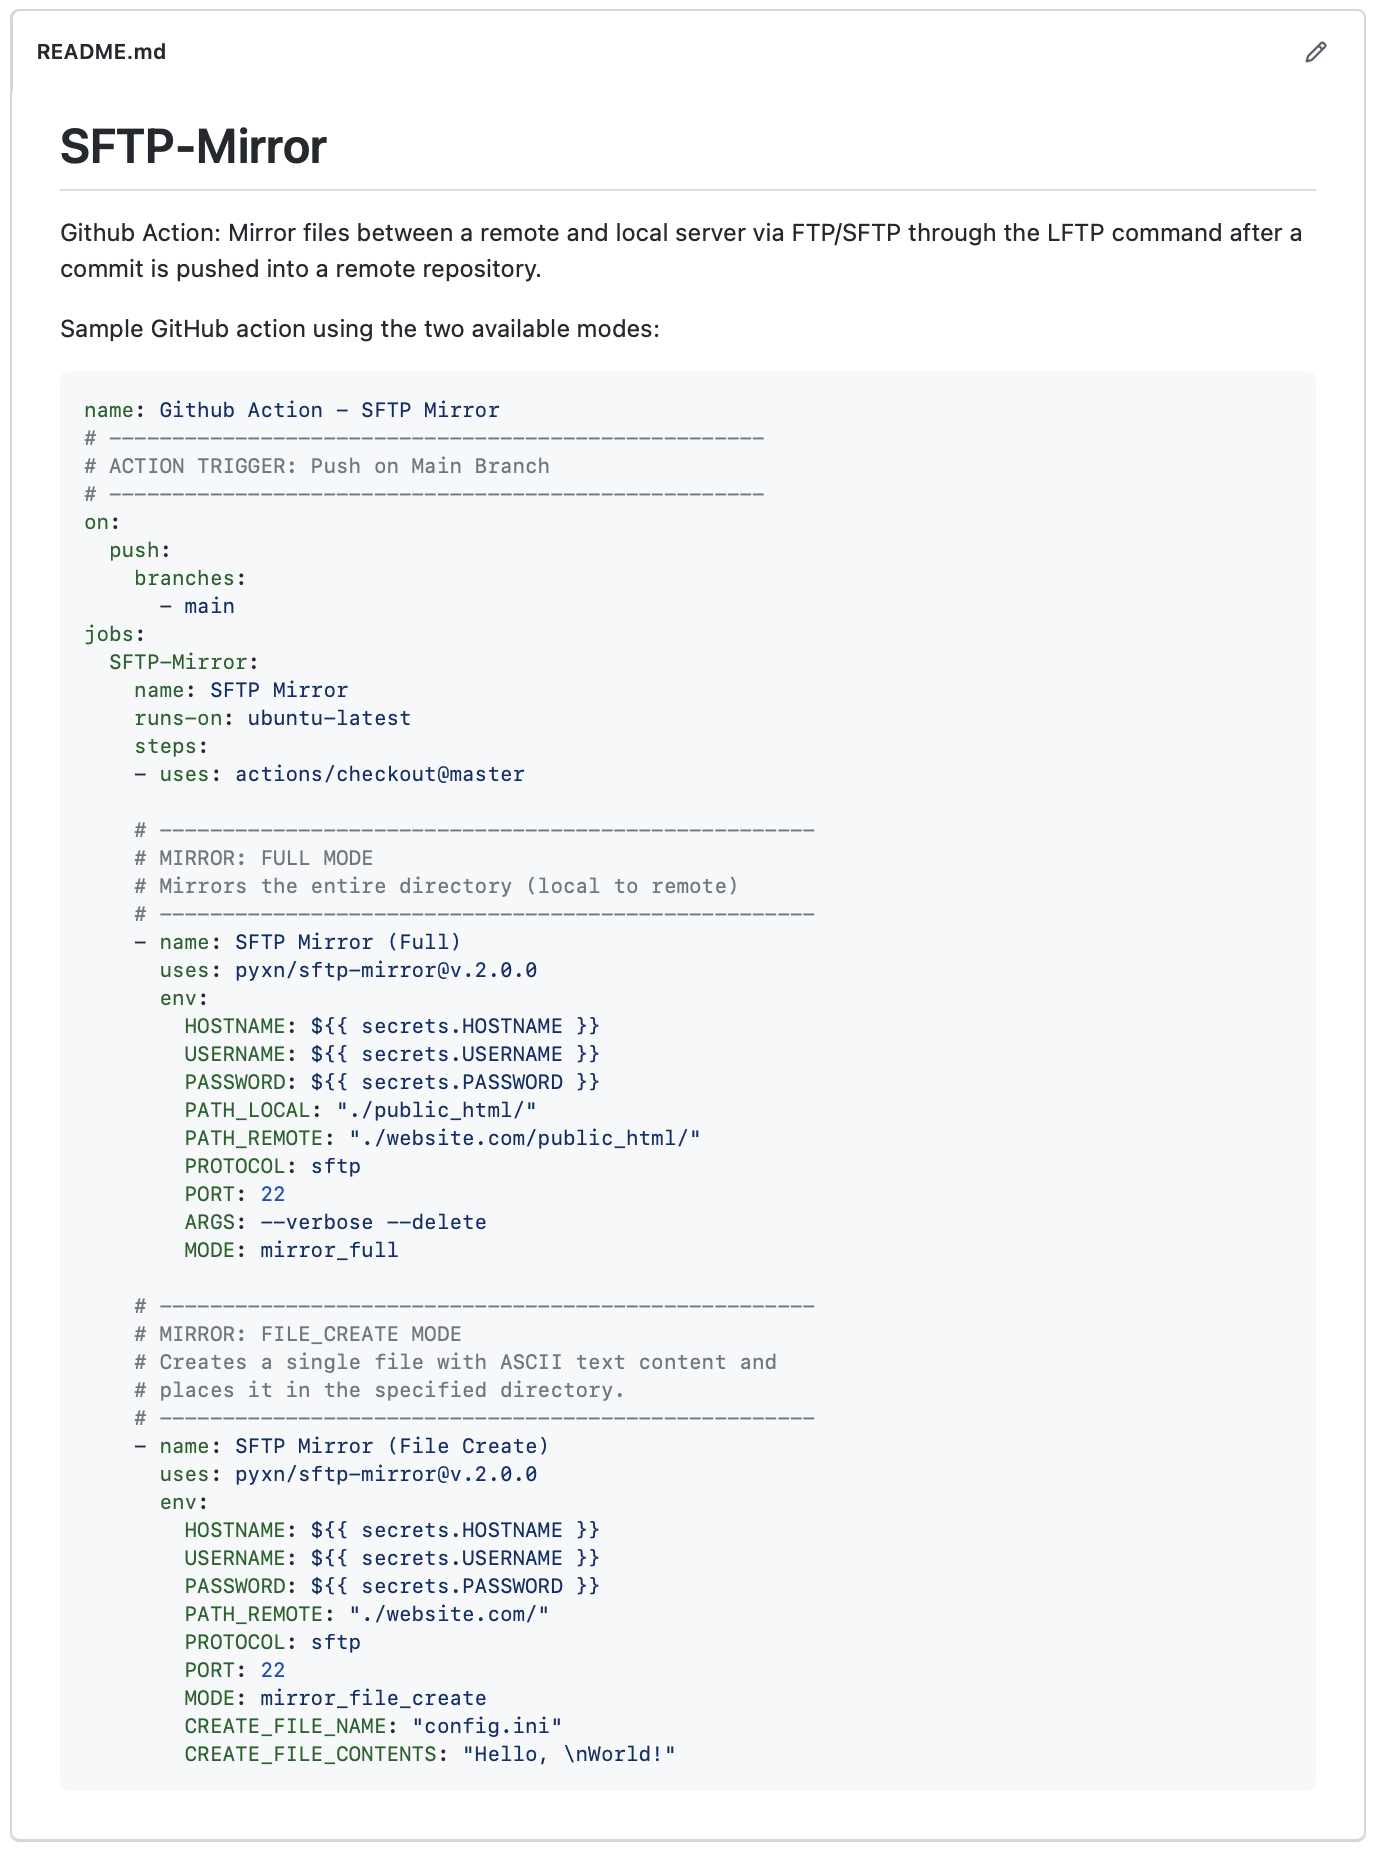
\includegraphics[width=4.4in]{images/25-sftp-mirror-usage.png}
	\caption{SFTP-Mirror: Usage Sample and Details}
 \end{figure}

\newpage
\subsection*{Installation Instructions}
The tool can be used by simply modifying the workflow files in the official repository, and input the new deployment location's configuration details on the workflow files directly or through GitHub secrets.

\subsubsection*{Installation File Directory}
The following screenshot displays where a developer might switch the configuration details of their own server to automatically deploy their own distributions.

\begin{figure}[htbp]
	\centering
	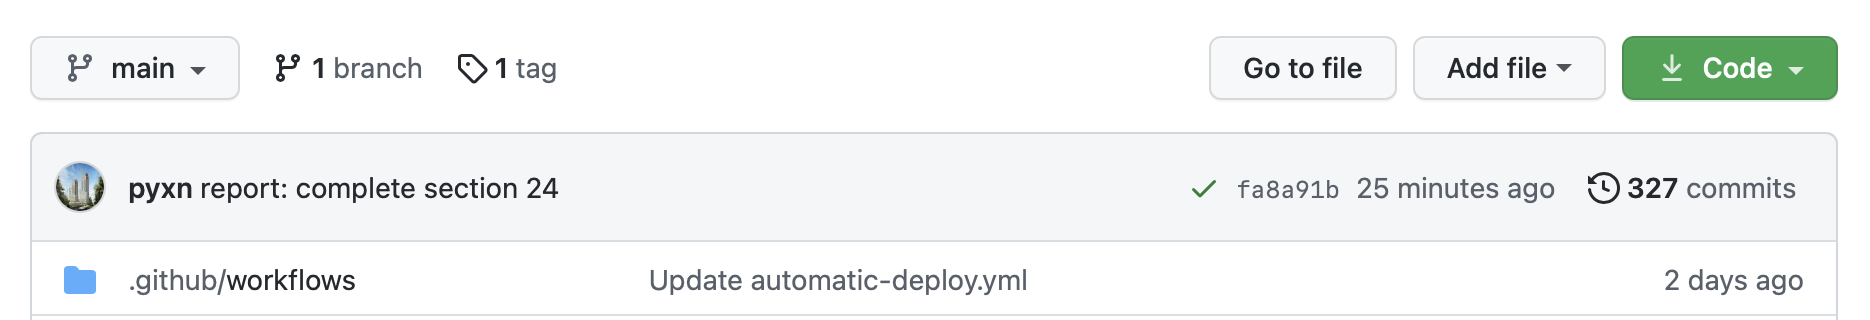
\includegraphics[width=\textwidth]{images/25-workflows.png}
	\caption{Location of Workflow Files}
 \end{figure}

 \subsubsection*{Installation Lines Sample}
In this screenshot, we can see the lines which can be replaced with the appropriate details for custom installation and deployment by other developers.
\begin{figure}[htbp]
	\centering
	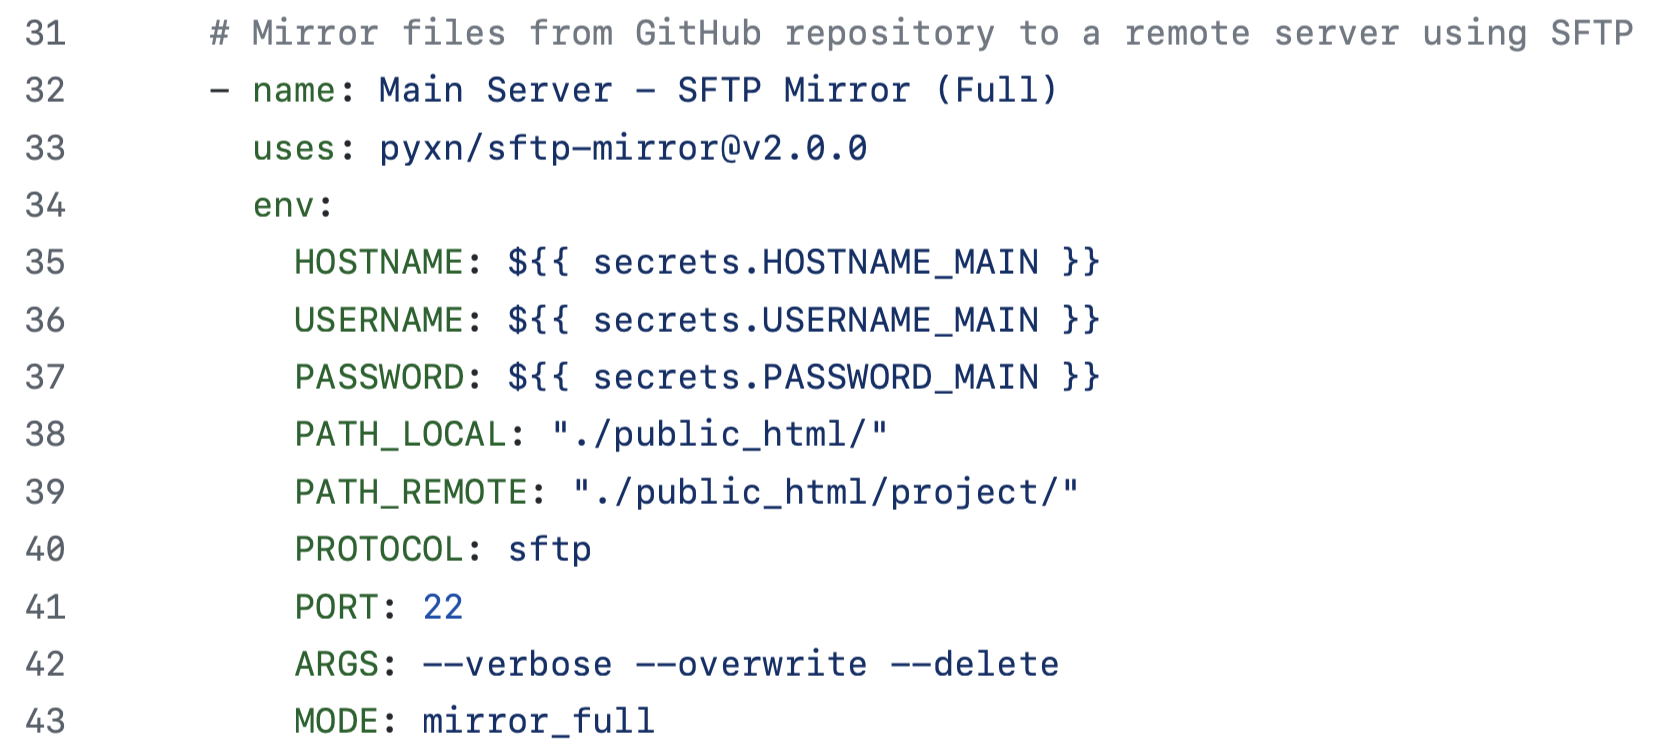
\includegraphics[width=\textwidth]{images/25-sftp-mirror-modify.png}
	\caption{Lines 35 to 39 can be replaced by developers with their own configuration details}
 \end{figure}

 \newpage
 \subsection*{GitHub Secrets}
To use GitHub secrets, developers can go to \lstinline{Settings}, then \lstinline{Secrets}, and then input their own secrets while using the same format as displayed in the official repository.

\begin{figure}[htbp]
	\centering
	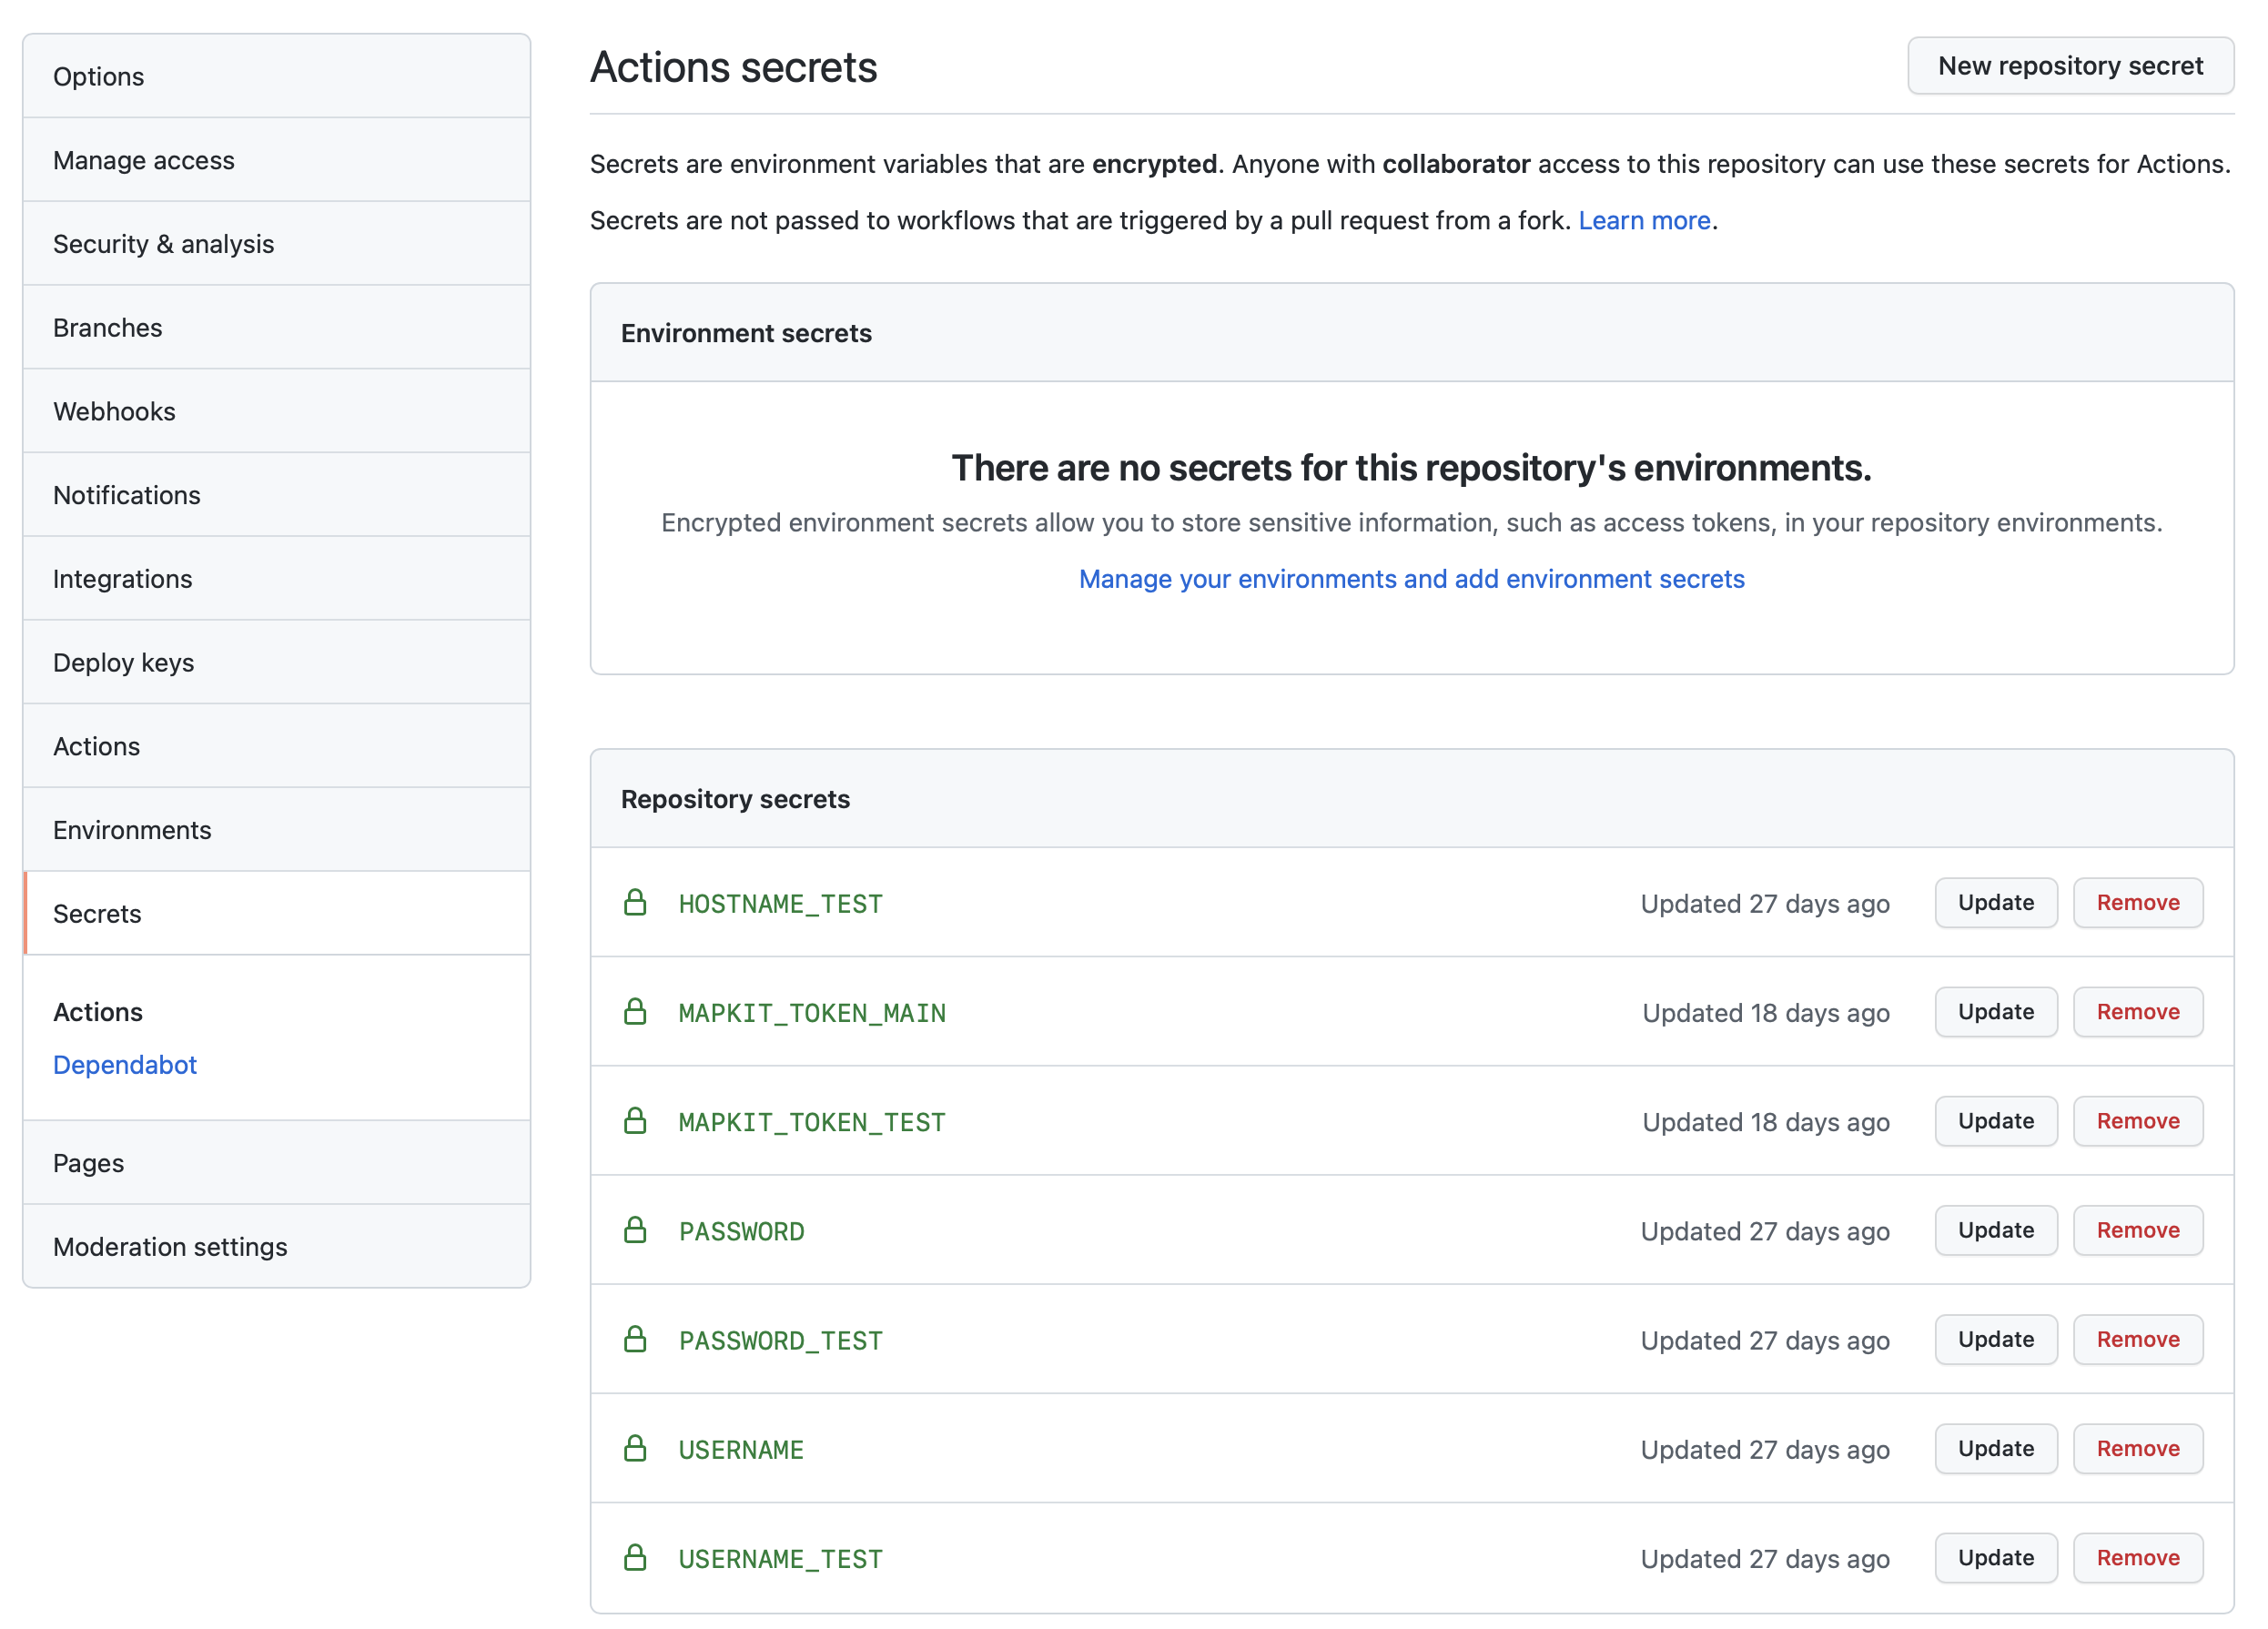
\includegraphics[width=\textwidth]{images/25-github-secrets.png}
	\caption{The GitHub Secrets page can be accessed in the repo settings}
 \end{figure}


 \newpage

% =====================================================================
%   26. ACCESSIBILITY
% =====================================================================
\section{Accessibility}

To check our website's accessibility score, we used the \textit{Experte Web and eCommerce Accessibility Checker} which can be found at \url{https://www.experte.com/accessibility}. 

\subsection*{Accessibility Testing Tool: Experte}
This tool checks how accessibly your website is. It crawls all crawlable pages, making sure that each page visited is correctly displayed by screen readers and any users which may use web accessibility features due to certain sense impairments.

\subsection*{Accessibility Scores}
The following screenshot displays a sample report of our highest accessibility scores, indicating that the website is highly accessible to users and indicate high accessibility compliance for the core and most important pages according to the high scores in the report.

\begin{figure}[htbp]
	\centering
	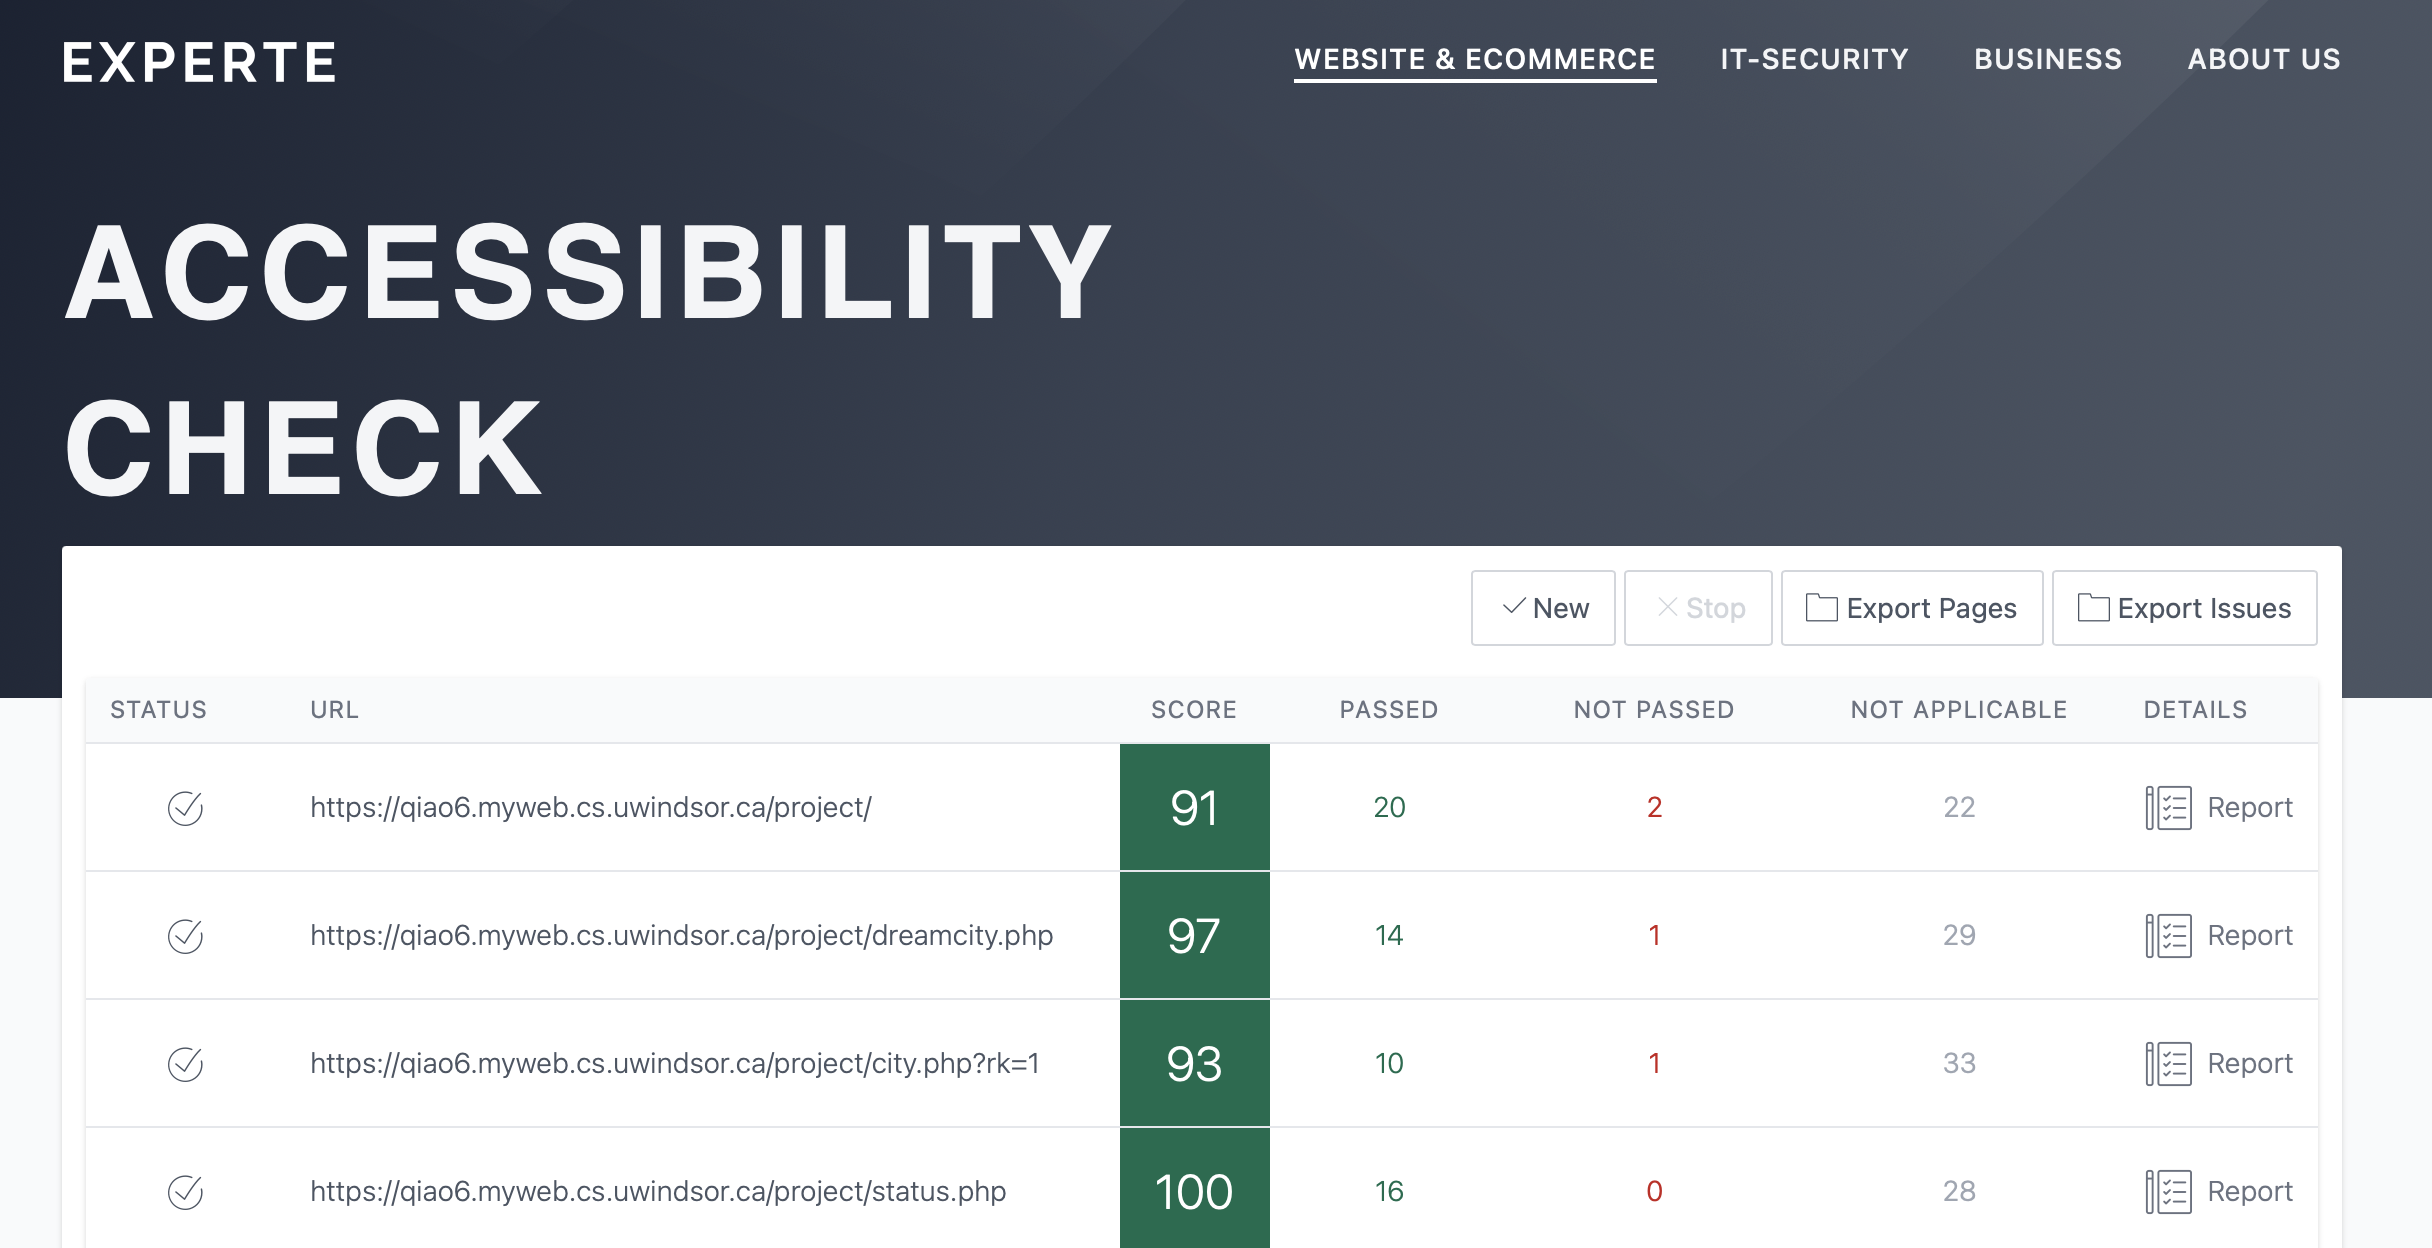
\includegraphics[width=\textwidth]{images/26-accessiblity-score.png}
	\caption{High Accessiblity Scores for Core Pages}
 \end{figure}

 \newpage


\subsection*{Accessibility Scores: Main}
The following screenshots display the main report for the homepage's accessibility score and passed checks, as well as the possible improvements that we can make to further improve the website's accessibility.

\begin{figure}[htbp]
	\centering
	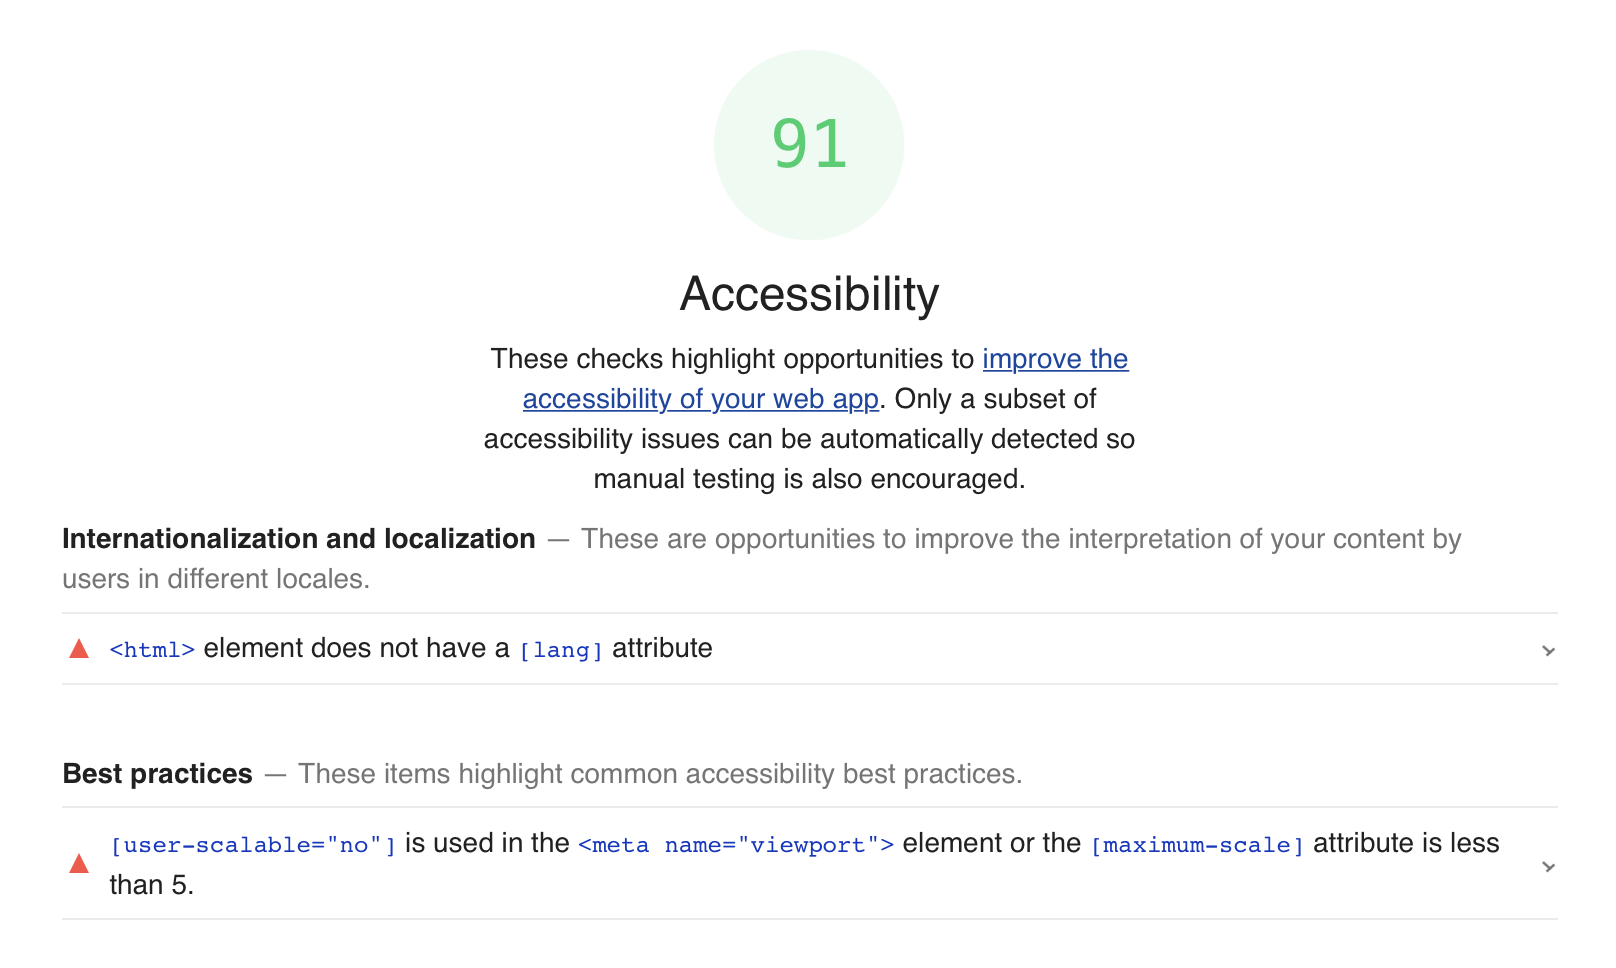
\includegraphics[width=\textwidth]{images/26-score-index.png}
	\caption{Possible Improvements According to the Report}
 \end{figure}

 \begin{figure}[htbp]
	\centering
	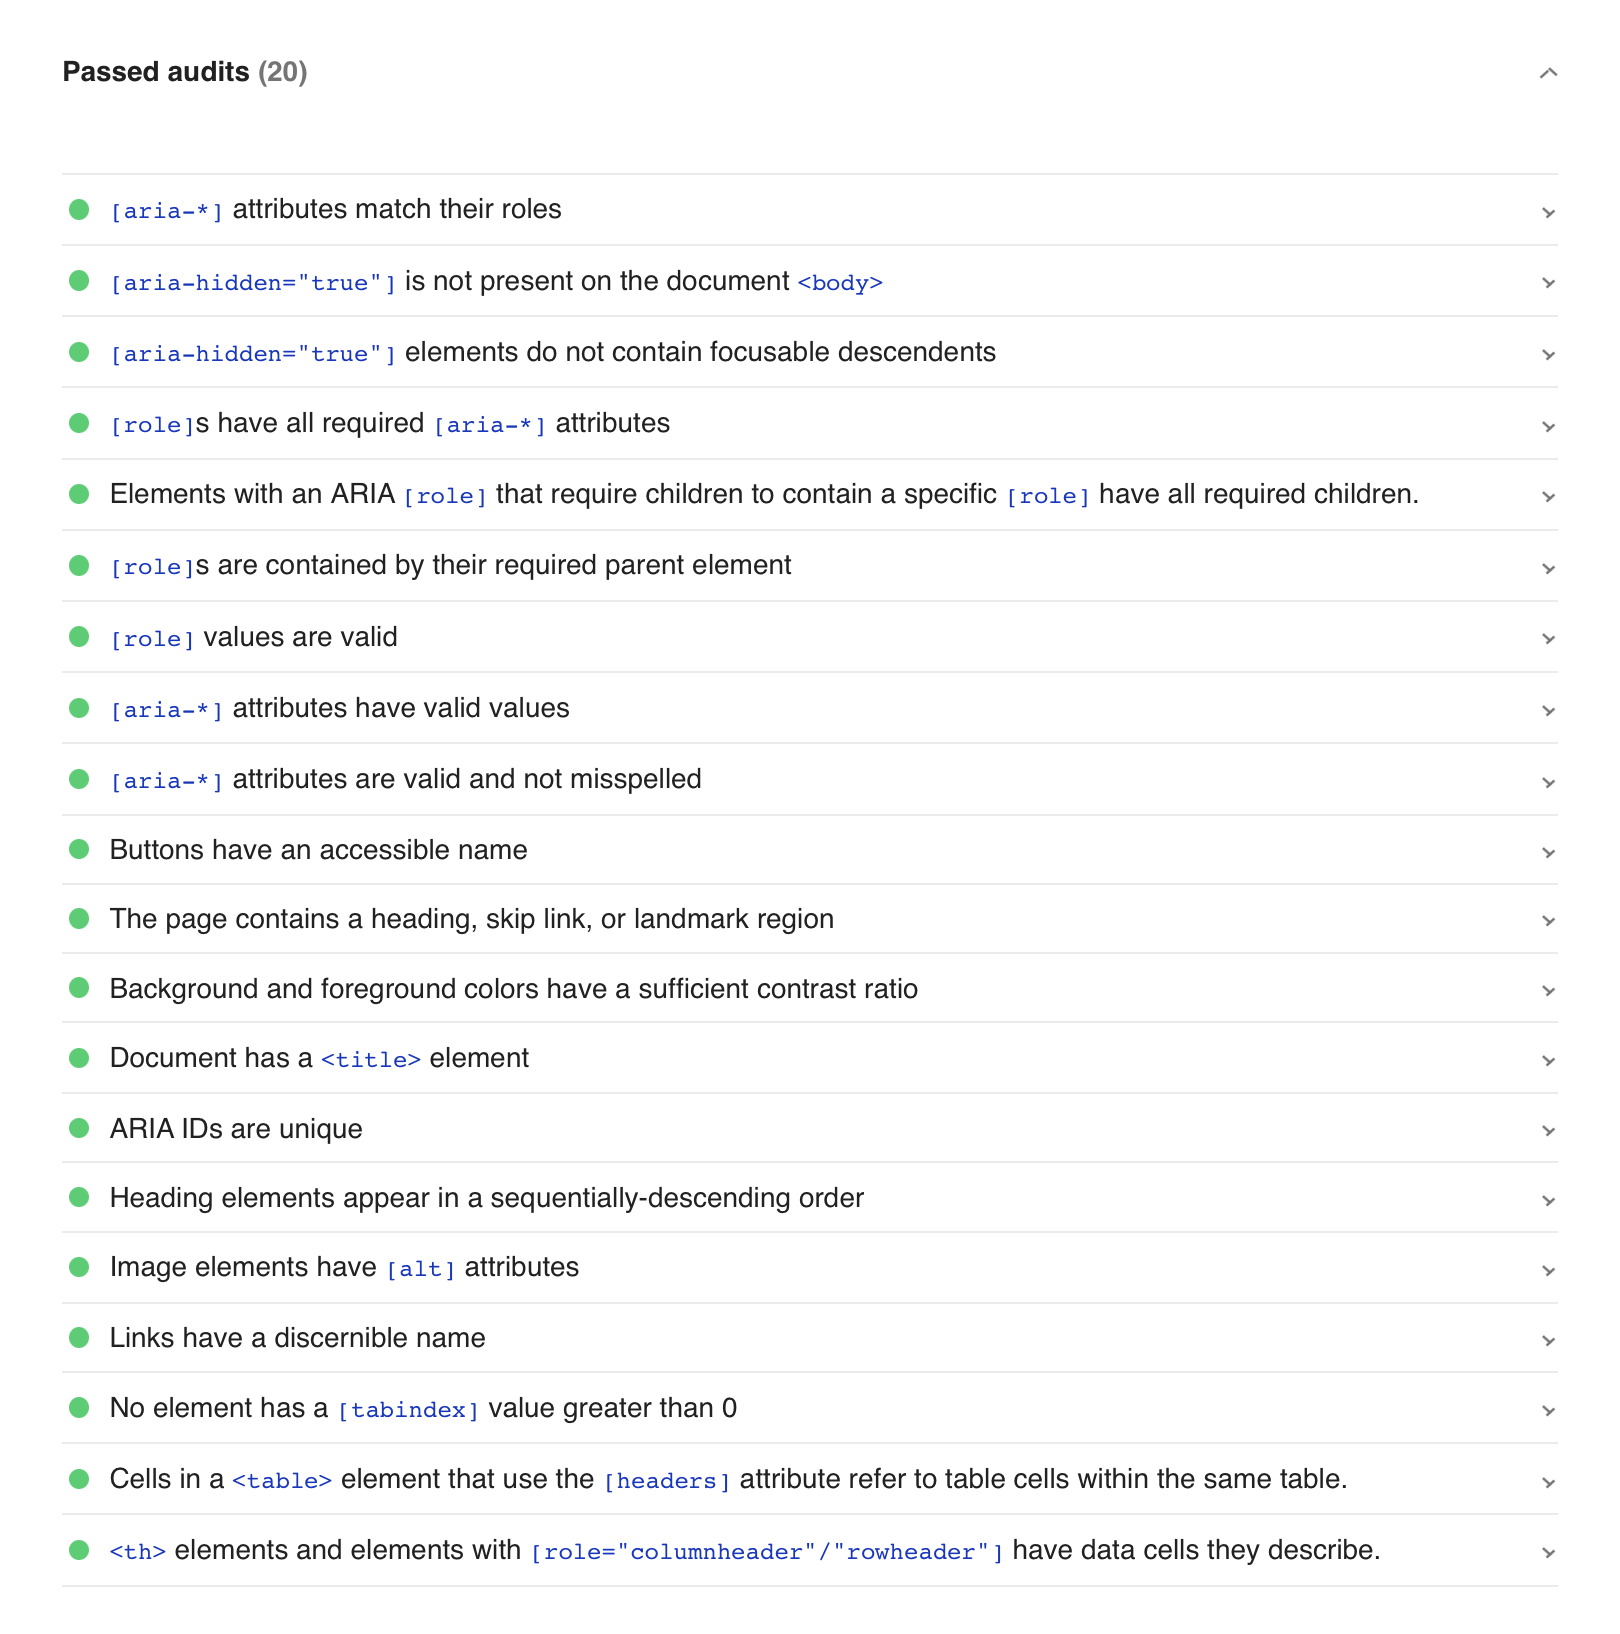
\includegraphics[width=\textwidth]{images/26-passed-index.png}
	\caption{Passed Checks for Website Accessibility}
 \end{figure}

 \newpage

% =====================================================================
%   27. MARK-UP VALIDATION SERVICE
% =====================================================================
\section{Mark-Up Validation Service}

For our mark-up validation testing, we ran the site on: \url{https://validator.w3.org/}. Attached below is the report and the result of the mark-up validation service. The following report indicates the possible improvements that we can make to improve the code on the website's most important, core pages:

\begin{figure}[htbp]
	\centering
	\includegraphics[width=\textwidth]{images/27-report-1.png}
	\caption{Validation Service Report (index.php) Part 1}
 \end{figure}

 \begin{figure}[htbp]
	\centering
	\includegraphics[width=\textwidth]{images/27-report-2.png}
	\caption{Validation Service Report (index.php) Part 2}
 \end{figure}

 \begin{figure}[htbp]
	\centering
	\includegraphics[width=\textwidth]{images/27-report-3.png}
	\caption{Validation Service Report (dreamcity.php)}
 \end{figure}

 \begin{figure}[htbp]
	\centering
	\includegraphics[width=\textwidth]{images/27-report-4.png}
	\caption{Validation Service Report (city.php)}
 \end{figure}


 \newpage

% =====================================================================
%   28. TESTING
% =====================================================================
\section{Testing}

\subsection*{Testing Strategy: AWS Test Server}
For testing, we utilized a custom AWS (Amazon Web Services) Lightsail Instance server. Using this custom test server, we are able to modify the development environment (such as using various versions of Linux, PHP, and MySQL) to test code compatibility for other server environments that other developers might use instead of the environment configuration we currently have on the main (MyWeb) server.

\subsubsection*{About AWS Lightsail}
AWS Lightsail is a light-weight virtual server instance service built on top of the popular AWS Elastic Compute (EC2) service. Using Lightsail, developers are able to deploy virtual servers in a few clicks and have full control of the development environment.

\subsubsection*{Lightsail Test Server Instance}
The following screenshot displays the test server instance that is currently running (\lstinline{yu-server-ubuntu-1}), as well as the publicly accessibly IP address where you can visit the test server. For convenience, we have also implemented a test domain name to test HTTPS/SSL compatibility with our project (\url{https://www.newcitybetterlife.com}).

\begin{figure}[htbp]
	\centering
	\includegraphics[width=\textwidth]{images/28-lightsail-instance.png}
	\caption{Our official AWS Lightsail Test Server Instance}
 \end{figure}

\subsection*{Testing Strategy: External Test Fork}
In addition to our test server, we also utilized a separate fork of the original repository to introduce new features that could potentially be site-breaking. While the main repository can deploy to both main and test servers, this external fork can only deploy to the test server for testing.

\begin{figure}[htbp]
	\centering
	\includegraphics[width=\textwidth]{images/28-external-fork.png}
	\caption{External fork to test possibly site-breaking features}
 \end{figure}

 \subsection*{Sample Development and Testing Workflows}
 The following screenshots display sample workflows using both the test server and the external fork. Using this strategy, we are able to mix and match the appropriate, universally-compatible code that is able to work on different environments. 
 
 The non-working features are abandoned after they are deployed and tested on the test server alone, while the working and completed features are merged into the main repository and then finally deployed to both main and test servers.

 \begin{figure}[htbp]
	\centering
	\includegraphics[width=\textwidth]{images/28-feature-abandon.png}
	\caption{Abandoning a non-working feature from the test fork}
 \end{figure}

 \begin{figure}[htbp]
	\centering
	\includegraphics[width=\textwidth]{images/28-feature-merge.png}
	\caption{Merge working features into the main repository}
 \end{figure}

 \newpage

% =====================================================================
%   29. TEAM MANAGEMENT
% =====================================================================
\section{Team Management}
For team management, we used a team and task management tool called \textit{ClickUp}. The tool can be accessed at \url{https://clickup.com/}.

\subsubsection*{Main Interface}
The following screenshot displays the main interface of the ClickUp team management tool. This screenshot also displays our group's completed tasks throughout the semester, which span for a total of 9 weeks and 4 days from the beginning of the first task to the due date of our final project report submission (June 8, 2021 to August 13, 2021).

\begin{figure}[htbp]
	\centering
	\includegraphics[width=\textwidth]{images/29-clickup-main.png}
	\caption{ClickUp Main Interface}
\end{figure}

\newpage

\subsection*{Tasks (Month-to-Month)}
The following screenshots display the tasks that have been completed or are currently in progress throughout the semester.

\subsubsection*{June 2021}
\begin{figure}[htbp]
	\centering
	\includegraphics[width=\textwidth]{images/29-clickup-month1.png}
	\caption{Completed Tasks for June 2021}
\end{figure}

\subsubsection*{July 2021}
\begin{figure}[htbp]
	\centering
	\includegraphics[width=\textwidth]{images/29-clickup-month2.png}
	\caption{Completed Tasks for July 2021}
\end{figure}

\subsubsection*{August 2021}
\begin{figure}[htbp]
	\centering
	\includegraphics[width=\textwidth]{images/29-clickup-month3.png}
	\caption{In Progress Tasks for August 2021}
\end{figure}


\newpage
\subsubsection*{Task Board}
The \textit{Board} section of ClickUp allows us to see an overview of the latest tasks that are currently in progress, and as well as the tasks that have been completed.

The task board is our primary gateway to accessing the latest tasks that are due and assigned to each team member. These tasks are organized by due date, priority, or any sorting setting that each team member may choose to have.

\begin{figure}[htbp]
	\centering
	\includegraphics[width=5.2in]{images/29-clickup-board.png}
	\caption{ClickUp Task Board}
\end{figure}

\subsubsection*{Calendar}
The calendar section displays the currently active and completed tasks within the selected timeframe. In the following screenshot, we can see the final task due for the group.

\begin{figure}[htbp]
	\centering
	\includegraphics[width=\textwidth]{images/29-clickup-calendar.png}
	\caption{ClickUp Calendar}
\end{figure}

\newpage
\subsubsection*{Task Creation}
From either the main interface or the board section, we are able to create the appropriate tasks that we need to complete and assign them to the appropriate team members.

The following screenshot displays the task creation screen, where our final task has just been created. The task is divided into subtasks, and each subtask is assigned to a team member. 

Each task is created with a due date (in this case we wanted to finish the final report 3 days early to finalize any missing features in the remaining days before the due date).

Once this task is created, each team member assigned a task or subtask is notified via email of the work assigned to them. Once the task is complete, we can check of and move the task/subtask into the \textit{Completed} area of the task board.

\begin{figure}[htbp]
	\centering
	\includegraphics[width=\textwidth]{images/29-clickup-task-creation.png}
	\caption{ClickUp Task Creation}
\end{figure}

\newpage

% =====================================================================
%   30. OVERALL COMPLETENESS AND ERROR-FREE FUNCTIONALITY
% =====================================================================
\section{Overall Completeness \& Error Free Functionality}

\subsection*{Sitemap}
The following screenshot shows our sitemap at the time of this writing, displaying the complete features available to end users and administrators of the website.

\begin{figure}[htbp]
	\centering
	\includegraphics[width=\textwidth]{images/30-sitemap.png}
	\caption{The Complete\textit{New City, Better Life} Sitemap}
 \end{figure}

\subsection*{Testing Completeness and Error-Free Functionality}
To test for the website's overall completeness and error-free functionality, we will go through test use cases of how an end user and administrator might navigate the website. 
For each step of the end-user or admin journey, we will be able to tell if the website works as intended with 100\% of the functionality working perfectly.

\newpage
\subsection*{Journey: End-User}

\subsubsection*{Visiting the Website}
The first step is for the user to visit the website using the main server URL: \url{qiao6.myweb.cs.uwindsor.ca/project/}. Visiting the homepage works as intended.
\begin{figure}[htbp]
	\centering
	\includegraphics[width=\textwidth]{images/30-journey-e01.png}
	\caption{Visiting the Homepage}
 \end{figure}

\newpage
\subsubsection*{Creating and Logging into an Account}
Since the website can be used with no account, we will test the website with an account to take out unnecessary steps of showing the end-user journey.

As displayed in the following screenshots, the login and authentication is working perfectly.

\begin{figure}[htbp]
	\centering
	\includegraphics[width=\textwidth]{images/30-journey-e02a.png}
	\caption{Creating an Account}
 \end{figure}

 \begin{figure}[htbp]
	\centering
	\includegraphics[width=\textwidth]{images/30-journey-e02b.png}
	\caption{Logged In After Account Creation}
 \end{figure}

\subsubsection*{Using the Map}
The map functionality works as intended in the homepage, with the most livable cities showing per province when a user hovers over a region.

\begin{figure}[htbp]
	\centering
	\includegraphics[width=4in]{images/30-journey-e03.png}
	\caption{Map Hover Works as Intended}
 \end{figure}

\newpage
 \subsubsection*{Accessing a Dynamic Page (Through the Top 10 Cities Table)}
A dynamic page is successfully generated and accessed when a record from the top 10 table in the homepage is clicked.

\begin{figure}[htbp]
	\centering
	\includegraphics[width=\textwidth]{images/30-journey-e04a.png}
	\caption{Clicking a Record}
 \end{figure}

 \begin{figure}[htbp]
	\centering
	\includegraphics[width=5in]{images/30-journey-e04b.png}
	\caption{Successful Dynamic Page Generation}
 \end{figure}

\newpage
 \subsubsection*{Accessing a Dynamic Page (Through the Dream City Page)}
 A dynamic page is successfully generated and accessed when using the dream city page to look for cities based on a certain criteria. Searching correctly displays the right cities and clicking a record successfully takes the user to the right dynamic page.

 \begin{figure}[htbp]
	\centering
	\includegraphics[width=5in]{images/30-journey-e05a.png}
	\caption{Successful City Search by Criteria: 1 million minimum population}
 \end{figure}

 \begin{figure}[htbp]
	\centering
	\includegraphics[width=4in]{images/30-journey-e05b.png}
	\caption{Successful Dynamic Page Generation}
 \end{figure}

 \newpage
 \subsubsection*{Adding a city to favorites}
Users can add cities to data-persistent list of favorites. In the following screenshot, we successfully click on the favorite heart to toggle it, and the favorited city then appears on the user's private profile page.

\begin{figure}[htbp]
	\centering
	\includegraphics[width=\textwidth]{images/30-journey-e06a.png}
	\caption{Toggling a city favorite}
 \end{figure}

 \begin{figure}[htbp]
	\centering
	\includegraphics[width=\textwidth]{images/30-journey-e06b.png}
	\caption{The favorited city appears on the users profile page}
 \end{figure}

 \newpage
 \subsubsection*{Changing User Details (End-user Side)}
Users can modify their account data using the user edit button located in their private profile page. The following screenshots show a user's account before and after a successful change.

\begin{figure}[htbp]
	\centering
	\includegraphics[width=\textwidth]{images/30-journey-e07a.png}
	\caption{The data of the current account}
 \end{figure}

 \begin{figure}[htbp]
	\centering
	\includegraphics[width=\textwidth]{images/30-journey-e07b.png}
	\caption{The updated data of the current account after change}
 \end{figure}

 \newpage
 \subsubsection*{Switching Themes}
If the user clicks the \lstinline{Switch Theme} button located on the bottom right of the page, the theme successfully switches to pink (from black earlier). The theme is applied to all pages the user can access, as shown with three (3) pages below.

\begin{figure}[htbp]
	\centering
	\includegraphics[width=5in]{images/30-journey-e08a.png}
	\caption{User Change Page}
 \end{figure}

 \begin{figure}[htbp]
	\centering
	\includegraphics[width=5in]{images/30-journey-e08b.png}
	\caption{System Status Page}
 \end{figure}

 \begin{figure}[htbp]
	\centering
	\includegraphics[width=5in]{images/30-journey-e08c.png}
	\caption{Home Page}
 \end{figure}

 \newpage
 \subsubsection*{Checking Website System Status}
Finally, the user can access the status page to check the status of the website. In the screenshot below, we can see that the website is fully operational, and the user can only see and access end-user features available to them.

\begin{figure}[htbp]
	\centering
	\includegraphics[width=\textwidth]{images/30-journey-e09.png}
	\caption{Website Status (End-User Perspective)}
 \end{figure}

 \newpage
 \subsubsection*{Logging Out}
Finally, let's go back to the homepage and try to logout. As you can see from the screenshot below, the navigation menu and the logged-in indicator reset to their original form. Logging out also removes access to account-only features such as the profile page and the favorites button. This indicates that our login and logout system is successfully working as intended.

\begin{figure}[htbp]
	\centering
	\includegraphics[width=3.5in]{images/30-journey-e10a.png}
	\caption{Website Status (End-User Perspective)}
 \end{figure}

\begin{figure}[htbp]
\centering
\includegraphics[width=3.5in]{images/30-journey-e10b.png}
\caption{Website Status (End-User Perspective)}
\end{figure}

 \subsubsection*{Journey: End-User - Conclusion}
This concludes our end-user test case, confirming that the complete end-user experience is working 100\% perfectly and as intended.

 \newpage
\subsection*{Journey: Administrator}
\subsubsection*{Logging In}
Next up, let's examine a test use-case of the Adminstrator journey. Let's go back to the status page to access the login system specifically for administrators. As shown in the screenshots below, the admin authentication and feature access elements work as intended.

\begin{figure}[htbp]
\centering
\includegraphics[width=4in]{images/30-journey-a01a.png}
\end{figure}

\begin{figure}[htbp]
\centering
\includegraphics[width=4in]{images/30-journey-a01b.png}
\caption{Logging in with an Admin Account}
\end{figure}

\begin{figure}[htbp]
\centering
\includegraphics[width=4.8in]{images/30-journey-a01c.png}
\caption{Status Page with Full Admin Feature Access}
\end{figure}

\newpage
\subsubsection*{Editing Users}
An adminstrator account can edit current user records, as you can see from the screenshots below, this functionality works as intended, showing how we  modify the test account we created earlier. To access editing functionality, a user must first be selected from the dropdown, and the admin must click the \textit{Edit} button. This is a security measure to prevent accidental changes.

\begin{figure}[htbp]
\centering
\includegraphics[width=4in]{images/30-journey-a02a.png}
\caption{Admin-Only Feature: Before User Edit}
\end{figure}

\begin{figure}[htbp]
\centering
\includegraphics[width=4in]{images/30-journey-a02b.png}
\caption{Admin-Only Feature: After User Edit}
\end{figure}

\newpage
\subsubsection*{Switching Admin Themes}
Admins also have access to an internal, administrator-area only theme switcher. From the screenshots below, we can see that switching to the other two themes (pink and yellow) work as intended.

\begin{figure}[htbp]
\centering
\includegraphics[width=2in]{images/30-journey-a03a.png}
\caption{Admin Internal UI: Yellow Theme}
\end{figure}

\begin{figure}[htbp]
\centering
\includegraphics[width=2in]{images/30-journey-a03b.png}
\caption{Admin Internal UI: Pink Theme}
\end{figure}

\begin{figure}[htbp]
\centering
\includegraphics[width=2in]{images/30-journey-a03c.png}
\caption{Admin Internal UI: Blue Theme}
\end{figure}


\newpage
\subsubsection*{Editing City Records}
Next let's test how an adminstrator account would edit an existing city record. If we go to the \textit{Edit Record} area from the current area (or from the status page), we can start editing any city record. We can access cities using either their rank number or their name.

In the following screenshots, we edit Langford by accessing it using its rank (1). Then, we change its scenery rating from 4 to 5. When we access the dynamic city page after saving the changes, we can see that record edit worked successfully.

\begin{figure}[htbp]
\centering
\includegraphics[width=4in]{images/30-journey-a04a.png}
\caption{Editing City with Rank = 1}
\end{figure}

\begin{figure}[htbp]
\centering
\includegraphics[width=4in]{images/30-journey-a04b.png}
\caption{City Page After the Change}
\end{figure}

\newpage
\subsubsection*{Creating System Notifications}
Back in the status page, adminstrator accounts can also create system notifications. In the following screenshots, we can observe the successful creation of a system notification.

\begin{figure}[htbp]
\centering
\includegraphics[width=4in]{images/30-journey-a05a.png}
\caption{Entering text for a new system notification}
\end{figure}

\begin{figure}[htbp]
\centering
\includegraphics[width=4in]{images/30-journey-a05b.png}
\caption{New system notification successfully created}
\end{figure}

\newpage
\subsubsection*{Deleting System Notifications}
If an administrator account is logged in, they are also able to delete system notification posts. A special button for post deletion appears right next to the system notification timestamp. Once we click this button, we can observe that the notification post is successfully deleted as intended.

\begin{figure}[htbp]
\centering
\includegraphics[width=\textwidth]{images/30-journey-a06a.png}
\caption{The Delete button shows up when an admin is logged in}
\end{figure}

\begin{figure}[htbp]
\centering
\includegraphics[width=5in]{images/30-journey-a06b.png}
\caption{The system notification page after post deletion}
\end{figure}

\newpage
\subsubsection*{Logging Out}
Finally, logged in adminstrators can log out of their accounts through three different pages, the status page, the edit user page, and the edit record page. As we can observe in the screenshots, the adminstrator is successfully logged out upon clicking one of these three log out links.

\begin{figure}[htbp]
\centering
\includegraphics[width=\textwidth]{images/30-journey-a07a.png}
\caption{Log out through edit user page}
\end{figure}

\begin{figure}[htbp]
\centering
\includegraphics[width=\textwidth]{images/30-journey-a07b.png}
\caption{Log out through edit record page}
\end{figure}

\begin{figure}[htbp]
\centering
\includegraphics[width=\textwidth]{images/30-journey-a07c.png}
\caption{Log out through status page}
\end{figure}

\newpage

\begin{figure}[htbp]
\centering
\includegraphics[width=\textwidth]{images/30-journey-a07d.png}
\caption{Status page on successful Log out}
\end{figure}

\subsubsection*{Journey: Administrator - Conclusion}
This concludes the user-journey for administrator accounts. As we have observed from the screenshots and the available flow of actions that are possible for admin accounts to take, we can see that the admin-side of the website works error-free and perfectly as intended.

\section{Conclusion}
In conclusion, the website works perfectly as intended. From a detailed testing of the user experience journey (for both end-users and administrators), we can observe that the website is indeed error-free in terms of all of its intended functionality | which is also fully-complete overall as intended.

\end{document}
